%%%%%%%%%%%%%%%%%%%%%%%%%%%%%%%%%%%%%%%%%%%%%%%%%%%%%%%%%%%%%%%%%%%%%%%%%%%%%%%%
%2345678901234567890123456789012345678901234567890123456789012345678901234567890
%        1         2         3         4         5         6         7         8

\documentclass[letterpaper, conference]{ieeeconf}  % Comment this line out if you need a4paper


% make changes take effect
\pagestyle{headings}
% adjust as needed
\addtolength{\footskip}{0\baselineskip}
\addtolength{\textheight}{-1\baselineskip}




%\documentclass[a4paper, 10pt, conference]{ieeeconf}      % Use this line for a4 paper

\IEEEoverridecommandlockouts                              % This command is only needed if 
                                                          % you want to use the \thanks command

% See the \addtolength command later in the file to balance the column lengths
% on the last page of the document

% The following packages can be found on http:\\www.ctan.org
\usepackage{graphicx} % for pdf, bitmapped graphics files
\usepackage{epstopdf}
%\usepackage{epsfig} % for postscript graphics files
%\usepackage{mathptmx} % assumes new font selection scheme installed
%\usepackage{times} % assumes new font selection scheme installed
\let\proof\relax
\let\endproof\relax
\usepackage{amsmath} % assumes amsmath package installed
\usepackage{amsthm}  % For special theorem style
\usepackage{amsfonts}
%\usepackage{amssymb}  % assumes amsmath package installed
\usepackage[dvipsnames]{xcolor}
\usepackage{tikz}
\usepackage{pgfplots}
\usetikzlibrary{shapes,arrows}
\usetikzlibrary{backgrounds}
\usepackage{multirow}
\usepackage[keeplastbox]{flushend}
%\usepackage{cite}  % Make sure that citation appear as [1]-[3] instead of [1], [2], [3]
\usepackage[utf8]{inputenc}    % utf8 support
\usepackage[T1]{fontenc}       % code for pdf file
\usepackage[USenglish]{babel}             %% language support
\usepackage{silence}  							%% For filtering warnings
\usepackage{csquotes}
% Add doi=false if no DOI
\usepackage[style=ieee,doi=false,isbn=false,date=year,backend=biber,maxbibnames=15,maxcitenames=2,mincitenames=1,uniquelist=false,uniquename=false,giveninits=true]{biblatex}
% Filter warnings issued by package biblatex starting with "Patching footnotes failed"
\WarningFilter{biblatex}{Patching footnotes failed}
\renewcommand*{\bibfont}{\footnotesize}		%% Use this for papers
\setlength{\biblabelsep}{\labelsep}
\bibliography{references}



\usepackage{pgfplots}
\pgfplotsset{compat=1.9}  % Prevent warning, pgf running in backwards compatibility mode anyway
%\usetikzlibrary{external}                       %% Create pdf figures from TikZ. Use PDFTeXify ...
%\tikzexternalize[prefix=tikz/]                  %% ... with --tex-option=--shell-escape switch.
\usepackage[capitalize]{cleveref}
\Crefname{figure}{Fig.}{Figs.}
\crefname{equation}{}{}
\Crefname{equation}{Equation}{Equations}
\newcommand{\crefrangeconjunction}{--}
\usepackage{subcaption}
\usepackage{xstring}
\usepackage{xparse}
\usepackage{siunitx}

\theoremstyle{plain}
\newtheorem{definition}{Definition}
\newtheorem{problem}{Problem}
\theoremstyle{remark}\newtheorem{remarkenv}{Remark}        %% remarks
\newenvironment{remark}{\begin{remarkenv}}%
	{\hfill$\lozenge$\end{remarkenv}}            %% end remark with a lozenge

% Table stuff
\usepackage{booktabs}
\usepackage{tabularx}
\newcolumntype{Y}{>{\raggedright\arraybackslash}X}
\setlength{\heavyrulewidth}{0.1em}
\newcommand{\otoprule}{\midrule[\heavyrulewidth]}
% Uncomment the following to get rid of badness warnings inside tables.
%\hbadness=\maxdimen
%\vbadness=\maxdimen
%\vfuzz=30pt
%\hfuzz=30pt

%\pgfplotsset{compat=newest} 
%\pgfplotsset{plot coordinates/math parser=false}

%Images path 
\graphicspath{ {figures/} }


\title{\LARGE \bf
	Real-world scenario mining for the assessment of automated vehicles
}

\author{Erwin de Gelder$^{1,2*}$, Jeroen Manders$^{1}$, Corrado Grappiolo$^{1}$, Jan-Pieter Paardekooper$^{1,3}$, \\ Olaf Op den Camp$^{1}$, Bart De Schutter$^{2}$%
\thanks{$^{1}$TNO, P.O. Box 756, 5700 AT Helmond, The Netherlands}%
\thanks{$^{2}$Delft University of Technology, Delft Center for Systems and Control, Delft, The Netherlands}%
\thanks{$^{3}$Radboud University, Donders Institute for Brain, Cognition and Behaviour, Nijmegen, The Netherlands}%
\thanks{$^{*}$Corresponding author. \newline E-mail address: {\tt\small erwin.degelder@tno.nl}}%
%\thanks{*This work was not supported by any organization}% <-this % stops a space
%\thanks{$^{1}$Albert Author is with Faculty of Electrical Engineering, Mathematics and Computer Science,
%        University of Twente, 7500 AE Enschede, The Netherlands
%        {\tt\small albert.author@papercept.net}}%
%\thanks{$^{2}$Bernard D. Researcheris with the Department of Electrical Engineering, Wright State University,
%        Dayton, OH 45435, USA
%        {\tt\small b.d.researcher@ieee.org}}%
}


\newlength\figurewidth
\newlength\figureheight
\definecolor{egocolor}{RGB}{220, 200, 200}
\definecolor{othervehicle}{RGB}{200, 220, 200}
\definecolor{staticenvironment}{RGB}{200, 200, 220}
\newlength{\tagheight}\setlength{\tagheight}{3em}
\newlength{\subjectwidth}\setlength{\subjectwidth}{6em}
\newlength{\descriptionwidth}\setlength{\descriptionwidth}{7em}
\newlength{\tagtotalwidth}\setlength{\tagtotalwidth}{27em}
\newlength{\egovehiclecruising}\setlength{\egovehiclecruising}{6em}
\newlength{\egovehicleaccelerating}\setlength{\egovehicleaccelerating}{10em}
\newlength{\egovehiclefollowing}\setlength{\egovehiclefollowing}{12em}
\newlength{\egovehiclechanging}\setlength{\egovehiclechanging}{9em}
\newlength{\itempos}\setlength{\itempos}{2em}
\newlength{\timepos}\setlength{\timepos}{2em}

\newlength{\tagsep}\setlength{\tagsep}{0.5em}
\newlength{\otherfollowing}\setlength{\otherfollowing}{5.5em}
\newlength{\otherchanging}\setlength{\otherchanging}{8em}
\newlength{\othernolead}\setlength{\othernolead}{9.5em}
\newlength{\cutinheight}\setlength{\cutinheight}{2.2em}
\newlength{\arrowheight}\setlength{\arrowheight}{0.8em}

\tikzstyle{block}=[minimum height=\tagheight, align=center, anchor=north east]
\tikzstyle{tag}=[block, draw, anchor=north west]
\tikzstyle{timeline}=[ultra thick, color=black]
\tikzstyle{showitem}=[dashed]
\tikzstyle{cutinline}=[ultra thick, color=red]



\usetikzlibrary{arrows,positioning}
\usetikzlibrary{arrows.meta}

% Notations
\newcommand{\symboldec}[2]{#1^{-}\left(#2\right)}
\newcommand{\symbolinc}[2]{#1^{+}\left(#2\right)}

\newcommand{\accelerationsymbol}{a}
\newcommand{\accelerationstart}{\accelerationsymbol_\mathrm{start}}
\newcommand{\accelerationcruise}{\accelerationsymbol_\mathrm{end}}
\newcommand{\defsym}{\equiv}
\newcommand{\indextarget}{i}
\newcommand{\lanechangethreshold}{\Delta_{\mathrm{l}}}
\newcommand{\lanechangespeed}{v_{\mathrm{lat}}}
\newcommand{\lineleftsymbol}{l}
\newcommand{\lineleft}[1]{\lineleftsymbol\left(#1\right)}
\newcommand{\lineleftdec}[1]{\symboldec{\lineleftsymbol}{#1}}
\newcommand{\lineleftinc}[1]{\symbolinc{\lineleftsymbol}{#1}}
\newcommand{\linerightsymbol}{r}
\newcommand{\lineright}[1]{\linerightsymbol\left(#1\right)}
\newcommand{\linerightdec}[1]{\symboldec{\linerightsymbol}{#1}}
\newcommand{\linerightinc}[1]{\symbolinc{\linerightsymbol}{#1}}
\newcommand{\nofngram}{n}
\newcommand{\sample}{k}
\newcommand{\sampledummy}{\tau}
\newcommand{\sampleenddec}[1]{\sample_{\mathrm{end}}^{-}\left(#1\right)}
\newcommand{\sampleendinc}[1]{\sample_{\mathrm{end}}^{+}\left(#1\right)}
\newcommand{\samplehorizon}{\sample_{\mathrm{h}}}
\newcommand{\sampleinit}{\sample_{0}}
\newcommand{\sampleaccevent}{\sample^{+}}
\newcommand{\sampledecevent}{\sample^{-}}
\newcommand{\samplescruising}{\sample_\mathrm{cruise}}
\newcommand{\sampleendleft}[1]{\sample_\mathrm{l,end}\left(#1\right)}
\newcommand{\sampleendright}[1]{\sample_\mathrm{r,end}\left(#1\right)}
\newcommand{\samplestartleft}[1]{\sample_\mathrm{l,start}\left(#1\right)}
\newcommand{\samplestartright}[1]{\sample_\mathrm{r,start}\left(#1\right)}
\newcommand{\speedsymbol}{v}
\newcommand{\speed}[1]{\speedsymbol\left(#1\right)}
\newcommand{\speedmax}[1]{\speedsymbol_\mathrm{max}\left(#1\right)}
\newcommand{\speedmin}[1]{\speedsymbol_\mathrm{min}\left(#1\right)}
\newcommand{\speeddec}[1]{\symboldec{\speedsymbol}{#1}}
\newcommand{\speedinc}[1]{\symbolinc{\speedsymbol}{#1}}
\newcommand{\speeddiff}{\Delta_{\speedsymbol}}
\newcommand{\speedtargetiabs}[2]{\speedsymbol_{#2}^{\mathrm{abs}}\left(#1\right)}
\newcommand{\speedtargetirel}[2]{\speedsymbol_{#2}^{\mathrm{rel}}\left(#1\right)}
\renewcommand{\time}{t}
\newcommand{\sampletime}{\time_\mathrm{s}}


\newcommand{\todo}[1]{\color{red}TO DO: #1 \color{black}}
%\usepackage{changebar}
\newcommand{\cstarta}{\color{black}}  % Changes since January 2, 2020
\newcommand{\cenda}{\color{black}}     % Changes since January 2, 2020
\newcommand{\cstartb}{\color{blue}}  % Changes since January 7, 2020
\newcommand{\cendb}{\color{black}}     % Changes since January 2, 2020

%\usepackage{setspace}
%\doublespacing


\begin{document}


\maketitle
\thispagestyle{empty}
\pagestyle{empty}


%%%%%%%%%%%%%%%%%%%%%%%%%%%%%%%%%%%%%%%%%%%%%%%%%%%%%%%%%%%%%%%%%%%%%%%%%%%%%%%%
\begin{abstract}
	\todo{Write abstract}
\end{abstract}

%%%%%%%%%%%%%%%%%%%%%%%%%%%%%%%%%%%%%%%%%%%%%%%%%%%%%%%%%%%%%%%%%%%%%%%%%%%%%%%%
\section{Introduction}
\label{sec:introduction}

TODO

\color{red}
For Arash and Hala: please use \\{\tt \textbackslash cref\{sec:introduction\}}\\ to refer to sections, figures etc. It automatically adds things as `Section': e.g., \cref{sec:introduction}.
\color{black}

The introduction contains: 
\begin{itemize}
	\item Setting up the context of automated driving
	\item Giving some background information about the hazard analysis and risk assessment in the ISO~26262 standard
	\item The gap (the problem) We currently have this as a separate chapter, we could move it to introduction depending on the length. 
	\item our contribution. 
	\item paper structure
\end{itemize}
\section{Problem formulation}
\label{sec:problem}

To formulate the scenario mining problem, we distinguish quantitative scenarios from qualitative scenarios, using the definitions of \emph{scenario} and \emph{scenario category} of \autocite{degelder2018ontology}:

\begin{definition}[Scenario]
	\label{def:scenario}
	A scenario is a quantitative description of the relevant characteristics of the ego vehicle, its activities and/or goals, its static environment, and its dynamic environment. In addition, a scenario contains all events that are relevant to the ego vehicle.
\end{definition}

\begin{definition}[Scenario category \autocite{degelder2018ontology}]
	\label{def:scenario category}
	A scenario category is a qualitative description of the ego vehicle, its activities and/or goals, its static environment, and its dynamic environment.
\end{definition}

\cstarta
A scenario category is an abstraction of a scenario and, therefore, a scenario category comprises multiple scenarios \autocite{degelder2018ontology}.
For example, the scenario category ``cut in'' comprises all possible cut-in scenarios. 
Given such a scenario category, our goal is to find all corresponding scenarios in a given data set. 
Hence, we define the scenario mining problem as follows:
\begin{problem}[Scenario mining]
	Given a scenario category, how to find all scenarios that correspond to this scenario category in a given data set?
\end{problem}
\cenda


\section{Data tagging}
\label{sec:tagging}

\begin{table*}
	\cstarta
	\centering
	\caption{\cstarta Tags that are considered in this paper.\cenda}
	\label{tab:tags}
	\begin{tabular}{llll}
		\toprule
		Subject & Description & Section & Possible tags \\ \otoprule
		Ego vehicle & Longitudinal activity & \cref{sec:longitudinal ego} & Accelerating, decelerating, cruising \\
		Ego vehicle & Lateral activity & \cref{sec:lateral ego} & Changing lane left, changing lane right, following lane \\
		Any other vehicle & Longitudinal activity & \cref{sec:longitudinal other vehicles} & Accelerating, braking, cruising \\
		Any other vehicle & Lateral activity & \cref{sec:lateral other vehicles} & Changing lane left, changing lane right, following lane \\
		Any other vehicle & Longitudinal state & \cref{sec:longitudinal state other vehicle} & In front of ego, behind ego \\
		Any other vehicle & Lateral state & \cref{sec:lateral state other vehicle} & Left of ego, right of ego, same lane as ego, unclear \\
		Any other vehicle & Lead vehicle & \cref{sec:lead vehicle} & Leader, no leader \\
		Static environment & On highway & \cref{sec:static environment} & Highway, no highway \\ 
		\bottomrule
	\end{tabular}
	\cenda
\end{table*}

\cstarta
Our method of scenario mining is divided into two steps. 
The first step consists in describing the data using \emph{tags} and the second step involves extracting the scenarios based on these tags. 
In this section, we explain how the \emph{tags} are determined. 
The scenario mining based on these tags is explained in the next section.

As described in \cref{def:scenario}, events and activities are constituents of a scenario. 
Part of the tags that we consider describe activities of the vehicles.
Therefore, we will use the definition of the term \emph{activity} of \autocite{degelder2018ontology}:\cenda
\begin{definition}[Activity \autocite{degelder2018ontology}]
	\label{def:activity}
	An activity quantitatively describes the time evolution of one or more state variables of an actor between two events.
\end{definition}
Because an activity starts and ends with an event, for describing the activities, we will first describe how we detect the events.

\cstarta
As an illustration, \cref{tab:tags} lists the tags that are considered for the case study in this paper. 
We distinguish between tags that describe the behavior of the ego vehicle, tags that describe the behavior and the state of any other vehicle, and tags that describe the static environment. \cenda
\begin{remark}
	\cstarta The tags in \cref{tab:tags} are sufficient for mining the scenarios of the scenario categories that we consider in our case study, see \cref{sec:case study}. However, when other scenario categories are considered, other tags might be necessary. The approach for mining the scenarios using the tags, however, is general and also applies when other tags are used. \cenda 
	\cstartc For example, for this paper we do not consider other road users than vehicles, but the proposed method also works if cyclists or pedestrians are considered.\cendc
\end{remark}

In the remainder of this section, we explain how the tags of \cref{tab:tags} are determined. 
Here, we assume that the data is sampled with a sample time of $\sampletime$.



\subsection{Longitudinal activity of the ego vehicle}
\label{sec:longitudinal ego}

We distinguish between three different longitudinal activities: ``accelerating'', ``decelerating'', and ``cruising''. 
The ego vehicle is performing either one of these activities. 
%To extract the activities from a dataset, we first extract the events.
\cstartc An acceleration activity starts at an acceleration event, so we will first describe how we detect an acceleration event.
\cendc

\cstarta To extract the longitudinal events, we might simply examine whether the acceleration of the vehicle is above or below a certain threshold. 
This approach, however, would be prone to sensor noise. 
That is why we use the speed difference within a certain sample window of length $\samplehorizon>0$, where $\samplehorizon$ is an integer.
Let $\speed{\sample}$ denote the speed of the ego vehicle at sample step $\sample$. 
Next, let us define the minimum and maximum speed between the current sample step $\sample$ and $\sample-\samplehorizon$:
\begin{align}
	\speedmin{\sample} &\defsym \min_{\sampledummy \in \left\{ \sample-\samplehorizon, \ldots, \sample \right\} } \speed{\sampledummy}, \\
	\speedmax{\sample} &\defsym \max_{\sampledummy \in \left\{ \sample-\samplehorizon, \ldots, \sample \right\} } \speed{\sampledummy}.
\end{align}\cenda
For detecting acceleration and decelerating events, the difference between the current speed and $\speedmin{\sample}$ and $\speedmax{\sample}$ are used:
\begin{align}
	\speedinc{\sample} &\defsym \speed{\sample} - \speedmin{\sample},\\
	\speeddec{\sample} &\defsym \speed{\sample} - \speedmax{\sample}.
\end{align}
\cstartd \Cref{fig:explain symbols} illustrates how $\speedmin{\sample}$, $\speedmax{\sample}$, $\speedinc{\sample}$, and $\speeddec{\sample}$ are calculated.
\cendd

\setlength{\figurewidth}{.9\linewidth}
\setlength{\figureheight}{.6\linewidth}
\begin{figure}
	\centering
	% This file was created by tikzplotlib v0.8.7.
\begin{tikzpicture}

\definecolor{color0}{rgb}{0.12156862745098,0.466666666666667,0.705882352941177}

\begin{axis}[
axis x line*=bottom,
axis y line*=left,
every x tick/.style={black},
every y tick/.style={black},
height=\figureheight,
tick align=outside,
tick pos=left,
width=\figurewidth,
x grid style={white!69.01960784313725!black},
xmin=0, xmax=16,
xtick style={color=black},
xtick={3,13},
xticklabels={\(\displaystyle k-k_h\),\(\displaystyle k\)},
y grid style={white!69.01960784313725!black},
ymin=0, ymax=30,
ytick style={color=black},
ytick={6.48176150995277,26.6384896175217},
yticklabels={\(\displaystyle v_{\mathrm{min}}(k)\),\(\displaystyle v_{\mathrm{max}}(k)\)}
]
\path [draw=black, fill=white]
(axis cs:13.6,26.6384896175217)
--(axis cs:14.1,25.1384896175217)
--(axis cs:13.6005,26.6384896175217)
--(axis cs:13.6005,18.1710298687663)
--(axis cs:13.5995,18.1710298687663)
--(axis cs:13.5995,26.6384896175217)
--(axis cs:13.1,25.1384896175217)
--cycle;
\path [draw=black, fill=white]
(axis cs:13.6,18.1710298687663)
--(axis cs:13.1,19.6710298687663)
--(axis cs:13.5995,18.1710298687663)
--(axis cs:13.5995,26.6384896175217)
--(axis cs:13.6005,26.6384896175217)
--(axis cs:13.6005,18.1710298687663)
--(axis cs:14.1,19.6710298687663)
--cycle;
\path [draw=black, fill=white]
(axis cs:13.6,6.48176150995277)
--(axis cs:13.1,7.98176150995277)
--(axis cs:13.5995,6.48176150995277)
--(axis cs:13.5995,18.1710298687663)
--(axis cs:13.6005,18.1710298687663)
--(axis cs:13.6005,6.48176150995277)
--(axis cs:14.1,7.98176150995277)
--cycle;
\path [draw=black, fill=white]
(axis cs:13.6,18.1710298687663)
--(axis cs:14.1,16.6710298687663)
--(axis cs:13.6005,18.1710298687663)
--(axis cs:13.6005,6.48176150995277)
--(axis cs:13.5995,6.48176150995277)
--(axis cs:13.5995,18.1710298687663)
--(axis cs:13.1,16.6710298687663)
--cycle;
\addplot [semithick, color0, mark=*, mark size=3, mark options={solid}, only marks]
table {%
0 12.2953146866099
1 18.8881758666537
2 20.0487810681893
3 26.6384896175217
4 25.7460113737956
5 19.6348856424945
6 18.4980426894777
7 11.6900416448795
8 9.09754897667893
9 7.94614004414408
10 6.48176150995277
11 10.4865437671727
12 10.1138044152746
13 18.1710298687663
14 21.8429753436936
15 20.3492135184764
16 21.2848438341475
};
\addplot [semithick, black, dashed]
table {%
3 0
3 30
};
\addplot [semithick, black, dashed]
table {%
13 0
13 30
};
\addplot [semithick, black, dashed]
table {%
0 6.48176150995277
16 6.48176150995277
};
\addplot [semithick, black, dashed]
table {%
0 26.6384896175217
16 26.6384896175217
};
\addplot [semithick, black, dashed]
table {%
12 18.1710298687663
14.6 18.1710298687663
};
\node at (axis cs:13.6,22.404759743144)[
  anchor=base west,
  text=black,
  rotate=0.0
]{$v^-(k)$};
\node at (axis cs:13.6,12.3263956893595)[
  anchor=base west,
  text=black,
  rotate=0.0
]{$v^+(k)$};
\end{axis}

\end{tikzpicture}

	\caption{\cstartd An example of a speed profile and how the variables $\speedmin{\sample}$, $\speedmax{\sample}$, $\speedinc{\sample}$, and $\speeddec{\sample}$ are calculated at a certain sample step $\sample$ with $\samplehorizon=10$.\cendd}
	\label{fig:explain symbols}
\end{figure}

First, we assume that the event at the start of the dataset is a cruising event at $\sample=\sampleinit$. Next, we go chronologically through the dataset. An acceleration event is happening at sample $\sample$ if any of the following conditions is true:
\begin{itemize}
	\item The vehicle is not performing an acceleration activity, i.e., the last event is not an acceleration event.
	\item \cstarta There has been a substantial speed increase between sample step $\sample-\samplehorizon$ and $\sample$, i.e., 
	\begin{equation}
		\label{eq:start acceleration}
		\speedinc{\sample} \geq \accelerationstart\samplehorizon\sampletime,
	\end{equation} \cenda
	where $\accelerationstart>0$ is a parameter.
	\item There is no lower speed in the near future, i.e.,
	\begin{equation}
		\label{eq:acceleration condition}
		\speedmin{\sample+\samplehorizon}=\speed{\sample}.
	\end{equation}
	\item There is a substantial speed difference during the activity, i.e., 
	\begin{equation}
		\label{eq:end acceleration condition}
		\left|\speed{\sampleendinc{\sample}} - \speed{\sample}\right| > \speeddiff,
	\end{equation}
	where \cstartc $\speeddiff>0$ is the minimum speed increase and \cendc $\sampleendinc{\sample}$ is controlled by the parameter $\accelerationcruise$ and \cstarta equals the first sample at which the speed increase is below a threshold\cenda:
	\begin{equation}
		\label{eq:end acceleration}
		\sampleendinc{\sample} \defsym \arg \min_{\sampledummy > \sample} \left\{ \sampledummy: \speedinc{\sampledummy+\samplehorizon} < \accelerationcruise\samplehorizon\sampletime \right\}.
	\end{equation}
\end{itemize}

\cstartd
A deceleration event is detected in a similar manner as an acceleration event. To detect a deceleration event, $-\speeddec{\cdot}$ substitutes $\speedinc{\cdot}$ in \cref{eq:start acceleration} and $\speedmin{\cdot}$ is substituted by $\speedmax{\cdot}$ in \cref{eq:acceleration condition}. Furthermore, $\sampleendinc{\cdot}$ in \cref{eq:end acceleration condition} is substituted by $\sampleenddec{\cdot}$, which is defined in a similar manner as $\sampleendinc{\cdot}$ in \cref{eq:end acceleration} but with $-\speeddec{\cdot}$ instead of $\speedinc{\cdot}$.\cendd

%A deceleration event is happening at sample $\sample$ if any of the following conditions is true:
%\begin{itemize}
%	\item The vehicle is not performing a decelerating activity, i.e., the last event is not a decelerating event.
%	\item \cstarta There has been a significant speed decrease, i.e., 
%	\begin{equation}
%		\label{eq:start deceleration}
%		\speeddec{\sample} \leq -\accelerationstart\samplehorizon\sampletime.
%	\end{equation} \cenda
%	\item There is no lower speed in the near future, i.e., $\speedmax{\sample}=\speed{\sample}$.
%	\item There is a significant speed difference during the activity, i.e., 
%	\begin{equation}
%		\speed{\sampleenddec{\sample}} - \speed{\sample} < -\speeddiff,
%	\end{equation}
%	with
%	\begin{equation}
%		\label{eq:end deceleration}
%		\sampleenddec{\sample} \defsym \arg \min_{\sampledummy > \sample} \left\{ \sampledummy\colon \speeddec{\sampledummy+\samplehorizon} > -\accelerationcruise\samplehorizon\sampletime \right\}.
%	\end{equation}
%\end{itemize}

Let $\sampleaccevent$ and $\sampledecevent$ denote the sample step of the most recent acceleration and decelerating event, respectively. A cruising event happens at sample step $\sample$ if the vehicle is not performing a cruising activity and if any of the following conditions is true:
\begin{itemize}
	\item $\sample > \sampleendinc{\sampleaccevent}$ when the vehicle is performing an acceleration activity.
	\item $\sample > \sampleenddec{\sampledecevent}$ when the vehicle is performing a decelerating activity.
\end{itemize}

\cstarta%
\Cref{fig:longitudinal activities} illustrates the longitudinal activities given a hypothetical speed profile (solid red line). The algorithm above described produces the activities ``cruising'', ``accelerating'', ``cruising'', ``decelerating'', and ``cruising''.
\cenda

\setlength{\figurewidth}{\linewidth}
\setlength{\figureheight}{0.7\linewidth}
\begin{figure}
	\centering
	% This file was created by tikzplotlib v0.8.7.
\begin{tikzpicture}

\definecolor{color0}{rgb}{1,0.2,0.2}
\definecolor{color1}{rgb}{0.2,1,0.2}
\definecolor{color2}{rgb}{0.2,0.2,1}

\begin{axis}[
axis x line*=bottom,
axis y line*=left,
every x tick/.style={black},
every y tick/.style={black},
height=\figureheight,
tick align=outside,
tick pos=left,
width=\figurewidth,
x grid style={white!69.01960784313725!black},
xlabel={Time [s]},
xmin=0, xmax=13,
xtick style={color=black},
y grid style={white!69.01960784313725!black},
ylabel={Speed [m/s]},
ymin=-5, ymax=17.5,
ytick style={color=black}
]
\addplot [line width=2.0pt, color0]
table {%
-2 7.5
-1.99 7.5
-1.98 7.5
-1.97 7.5
-1.96 7.5
-1.95 7.5
-1.94 7.5
-1.93 7.5
-1.92 7.5
-1.91 7.5
-1.9 7.5
-1.89 7.5
-1.88 7.5
-1.87 7.5
-1.86 7.5
-1.85 7.5
-1.84 7.5
-1.83 7.5
-1.82 7.5
-1.81 7.5
-1.8 7.5
-1.79 7.5
-1.78 7.5
-1.77 7.5
-1.76 7.5
-1.75 7.5
-1.74 7.5
-1.73 7.5
-1.72 7.5
-1.71 7.5
-1.7 7.5
-1.69 7.5
-1.68 7.5
-1.67 7.5
-1.66 7.5
-1.65 7.5
-1.64 7.5
-1.63 7.5
-1.62 7.5
-1.61 7.5
-1.6 7.5
-1.59 7.5
-1.58 7.5
-1.57 7.5
-1.56 7.5
-1.55 7.5
-1.54 7.5
-1.53 7.5
-1.52 7.5
-1.51 7.5
-1.5 7.5
-1.49 7.5
-1.48 7.5
-1.47 7.5
-1.46 7.5
-1.45 7.5
-1.44 7.5
-1.43 7.5
-1.42 7.5
-1.41 7.5
-1.4 7.5
-1.39 7.5
-1.38 7.5
-1.37 7.5
-1.36 7.5
-1.35 7.5
-1.34 7.5
-1.33 7.5
-1.32 7.5
-1.31 7.5
-1.3 7.5
-1.29 7.5
-1.28 7.5
-1.27 7.5
-1.26 7.5
-1.25 7.5
-1.24 7.5
-1.23 7.5
-1.22 7.5
-1.21 7.5
-1.2 7.5
-1.19 7.5
-1.18 7.5
-1.17 7.5
-1.16 7.5
-1.15 7.5
-1.14 7.5
-1.13 7.5
-1.12 7.5
-1.11 7.5
-1.1 7.5
-1.09 7.5
-1.08 7.5
-1.07 7.5
-1.06 7.5
-1.05 7.5
-1.04 7.5
-1.03 7.5
-1.02 7.5
-1.01 7.5
-0.999999999999999 7.5
-0.989999999999999 7.5
-0.979999999999999 7.5
-0.969999999999999 7.5
-0.959999999999999 7.5
-0.949999999999999 7.5
-0.939999999999999 7.5
-0.929999999999999 7.5
-0.919999999999999 7.5
-0.909999999999999 7.5
-0.899999999999999 7.5
-0.889999999999999 7.5
-0.879999999999999 7.5
-0.869999999999999 7.5
-0.859999999999999 7.5
-0.849999999999999 7.5
-0.839999999999999 7.5
-0.829999999999999 7.5
-0.819999999999999 7.5
-0.809999999999999 7.5
-0.799999999999999 7.5
-0.789999999999999 7.5
-0.779999999999999 7.5
-0.769999999999999 7.5
-0.759999999999999 7.5
-0.749999999999999 7.5
-0.739999999999999 7.5
-0.729999999999999 7.5
-0.719999999999999 7.5
-0.709999999999999 7.5
-0.699999999999999 7.5
-0.689999999999999 7.5
-0.679999999999999 7.5
-0.669999999999999 7.5
-0.659999999999999 7.5
-0.649999999999999 7.5
-0.639999999999999 7.5
-0.629999999999999 7.5
-0.619999999999999 7.5
-0.609999999999999 7.5
-0.599999999999999 7.5
-0.589999999999999 7.5
-0.579999999999999 7.5
-0.569999999999999 7.5
-0.559999999999999 7.5
-0.549999999999999 7.5
-0.539999999999999 7.5
-0.529999999999999 7.5
-0.519999999999999 7.5
-0.509999999999999 7.5
-0.499999999999999 7.5
-0.489999999999999 7.5
-0.479999999999999 7.5
-0.469999999999999 7.5
-0.459999999999999 7.5
-0.449999999999999 7.5
-0.439999999999999 7.5
-0.429999999999999 7.5
-0.419999999999999 7.5
-0.409999999999999 7.5
-0.399999999999999 7.5
-0.389999999999999 7.5
-0.379999999999999 7.5
-0.369999999999999 7.5
-0.359999999999999 7.5
-0.349999999999999 7.5
-0.339999999999999 7.5
-0.329999999999999 7.5
-0.319999999999999 7.5
-0.309999999999998 7.5
-0.299999999999998 7.5
-0.289999999999998 7.5
-0.279999999999998 7.5
-0.269999999999998 7.5
-0.259999999999998 7.5
-0.249999999999998 7.5
-0.239999999999998 7.5
-0.229999999999998 7.5
-0.219999999999998 7.5
-0.209999999999998 7.5
-0.199999999999998 7.5
-0.189999999999998 7.5
-0.179999999999998 7.5
-0.169999999999998 7.5
-0.159999999999998 7.5
-0.149999999999998 7.5
-0.139999999999998 7.5
-0.129999999999998 7.5
-0.119999999999998 7.5
-0.109999999999998 7.5
-0.0999999999999983 7.5
-0.0899999999999983 7.5
-0.0799999999999983 7.5
-0.0699999999999983 7.5
-0.0599999999999983 7.5
-0.0499999999999983 7.5
-0.0399999999999983 7.5
-0.0299999999999983 7.5
-0.0199999999999982 7.5
-0.00999999999999823 7.5
0 7.50882026172984
0.01 7.51082104777167
0.02 7.5157147376922
0.03 7.52691920368821
0.04 7.53625699363896
0.05 7.53137060423958
0.06 7.53612104632721
0.07 7.53536426028572
0.08 7.53484816602675
0.09 7.53690115853644
0.1 7.53762137639225
0.11 7.54489274392706
0.12 7.5486979325528
0.13 7.54930630763526
0.14 7.55152562379899
0.15 7.55319399543586
0.16 7.56066439080165
0.17 7.55963859948282
0.18 7.56120393799107
0.19 7.55693345929456
0.2 7.54416851021539
0.21 7.54743660319259
0.22 7.55175878418689
0.23 7.54804795908486
0.24 7.5593967322048
0.25 7.5521249038318
0.26 7.55235369641831
0.27 7.55141777716818
0.28 7.55908167323997
0.29 7.56642846708948
0.3 7.56720320421796
0.31 7.56909401681597
0.32 7.56465508807782
0.33 7.5547511057367
0.34 7.55301154499007
0.35 7.55379328983559
0.36 7.55994474323923
0.37 7.56595664248315
0.38 7.56402000839611
0.39 7.56250849464324
0.4 7.5572657298179
0.41 7.550165640132
0.42 7.54163428917888
0.43 7.55138816615504
0.44 7.54883990524628
0.45 7.54664953373822
0.46 7.54038555693797
0.47 7.54427300871713
0.48 7.53620351947934
0.49 7.53513981807827
0.5 7.53066248527231
0.51 7.5325969977616
0.52 7.53004297207376
0.53 7.52413981115315
0.54 7.52399890001145
0.55 7.52614055936411
0.56 7.52647314547602
0.57 7.52798550496472
0.58 7.52481389449631
0.59 7.52300018866638
0.6 7.5196378864275
0.61 7.5178401206198
0.62 7.51377438920957
0.63 7.50514297619792
0.64 7.50603010690918
0.65 7.50402120222814
0.66 7.49587021049331
0.67 7.49818412177094
0.68 7.49364762994903
0.69 7.49390735692801
0.7 7.49755280973889
0.71 7.49819772429268
0.72 7.5038947277154
0.73 7.49772059861363
0.74 7.49973230681952
0.75 7.49630825636482
0.76 7.49195427061891
0.77 7.48906002229508
0.78 7.48750225963445
0.79 7.4877830863456
0.8 7.48195733714168
0.81 7.48646146957645
0.82 7.4887897817751
0.83 7.48110856334372
0.84 7.48854982431269
0.85 7.49802927019285
0.86 7.50392316804865
0.87 7.50302354386958
0.88 7.49766978076203
0.89 7.50294203939669
0.9 7.50092615466182
0.91 7.50703838001373
0.92 7.50807975490412
0.93 7.51296295008654
0.94 7.51474478207241
0.95 7.51827764791337
0.96 7.51833014801697
0.97 7.5272595004865
0.98 7.52789406095002
0.99 7.52990400776724
1 7.53931976125252
1.01 7.53258096594681
1.02 7.52622854095438
1.03 7.53107552449517
1.04 7.5252099074696
1.05 7.53492801339785
1.06 7.53285991849405
1.07 7.52912264443685
1.08 7.53873735456925
1.09 7.54613992852642
1.1 7.55547772332855
1.11 7.56000794661993
1.12 7.55570181819466
1.13 7.56525214296015
1.14 7.56391212610539
1.15 7.56792440808438
1.16 7.57266066792325
1.17 7.57188561745779
1.18 7.57495601430952
1.19 7.57956704766735
1.2 7.58144917532313
1.21 7.57595217137021
1.22 7.57744336224124
1.23 7.58407529172468
1.24 7.58060245242602
1.25 7.57985427972438
1.26 7.57767851196577
1.27 7.58692483060817
1.28 7.59028630439323
1.29 7.59232361357444
1.3 7.58847403320221
1.31 7.59117027915867
1.32 7.58779861585538
1.33 7.58795776864676
1.34 7.58477853825486
1.35 7.58816070472959
1.36 7.59104365881267
1.37 7.59000216503478
1.38 7.59198219859809
1.39 7.58651689105443
1.4 7.57906060309091
1.41 7.58125756159723
1.42 7.58209092907409
1.43 7.58526608625855
1.44 7.59718181013287
1.45 7.60190420756782
1.46 7.5973400964406
1.47 7.60292517788108
1.48 7.59634564082852
1.49 7.59403771780445
1.5 7.59369650977783
1.51 7.60226322338607
1.52 7.59853944927583
1.53 7.59440725658254
1.54 7.59391499396041
1.55 7.5905976025286
1.56 7.59623078213913
1.57 7.59083112459732
1.58 7.58509378133526
1.59 7.58290468111154
1.6 7.58041451885808
1.61 7.59006217912716
1.62 7.59480928316179
1.63 7.59524703936872
1.64 7.58911986177456
1.65 7.59334167665657
1.66 7.58834059991962
1.67 7.58091674443574
1.68 7.5874568933975
1.69 7.58994160645712
1.7 7.59574590057603
1.71 7.59883953884074
1.72 7.60492369190025
1.73 7.60376856393375
1.74 7.60099734972483
1.75 7.60710532231624
1.76 7.60608827399537
1.77 7.60594052510662
1.78 7.60726286258903
1.79 7.61125025838416
1.8 7.61368028882789
1.81 7.6113055323608
1.82 7.61288744034664
1.83 7.60687042458551
1.84 7.61539658184065
1.85 7.61308629356262
1.86 7.61356437686547
1.87 7.62012520226178
1.88 7.62302738727982
1.89 7.63764246025686
1.9 7.63837817570824
1.91 7.64721343005498
1.92 7.65481701596385
1.93 7.65707654847514
1.94 7.6680929317778
1.95 7.67593520012169
1.96 7.68879415287776
1.97 7.70221167364758
1.98 7.72262785339398
1.99 7.73921049314116
2 7.74756458395145
2.01 7.75686768806357
2.02 7.77316598604301
2.03 7.78754230469662
2.04 7.80214296232711
2.05 7.80575818210555
2.06 7.81763655148356
2.07 7.82624639693753
2.08 7.84024601993274
2.09 7.85265526798453
2.1 7.87040616252499
2.11 7.88549225360095
2.12 7.90322389341149
2.13 7.91499179792782
2.14 7.92466956664822
2.15 7.93731931818221
2.16 7.9522342161129
2.17 7.96942997479068
2.18 7.99632651954413
2.19 8.01201523378583
2.2 8.02343550878337
2.21 8.03820559990487
2.22 8.05268762003164
2.23 8.07219502740051
2.24 8.08189104232828
2.25 8.09990735229928
2.26 8.11868988498911
2.27 8.13815079017011
2.28 8.15376420982529
2.29 8.17147460117661
2.3 8.18355429663169
2.31 8.20058769721488
2.32 8.2176733898348
2.33 8.23955364006611
2.34 8.253572727907
2.35 8.27727871841555
2.36 8.304551141138
2.37 8.31400121601293
2.38 8.33593250966683
2.39 8.35911704984198
2.4 8.37572986471422
2.41 8.39354350564257
2.42 8.41267910275464
2.43 8.43099014835763
2.44 8.44924508351239
2.45 8.46066506448074
2.46 8.48622672230466
2.47 8.51142481526484
2.48 8.52715799396882
2.49 8.53962587232981
2.5 8.56203119671207
2.51 8.57895225686301
2.52 8.59946202267961
2.53 8.61766538059389
2.54 8.64092307434924
2.55 8.66419682006752
2.56 8.6803688331752
2.57 8.69325201339822
2.58 8.70513732141155
2.59 8.72798921830709
2.6 8.74184492201816
2.61 8.75911084024667
2.62 8.77592927005442
2.63 8.79546643357307
2.64 8.80558503454384
2.65 8.82632892752781
2.66 8.84874838264698
2.67 8.8689904930822
2.68 8.88723606222371
2.69 8.90752306305505
2.7 8.92931829478325
2.71 8.93525533100112
2.72 8.96483489254237
2.73 8.98658535915581
2.74 9.00312331624388
2.75 9.02096854936794
2.76 9.04323725825469
2.77 9.06245673855951
2.78 9.07210331622061
2.79 9.1022257805274
2.8 9.12147307724124
2.81 9.14637394079982
2.82 9.1627136915609
2.83 9.19019557683213
2.84 9.21142729527659
2.85 9.23427151444897
2.86 9.24884524761823
2.87 9.27470097406665
2.88 9.29795006488932
2.89 9.32425929603714
2.9 9.34091885823894
2.91 9.35831372264663
2.92 9.38963330613505
2.93 9.40413322702145
2.94 9.42325347851805
2.95 9.44873793533107
2.96 9.46902656016964
2.97 9.49174132856841
2.98 9.50954408342209
2.99 9.53119436286133
3 9.54446172860265
3.01 9.57255238200074
3.02 9.5917615617751
3.03 9.60816067075512
3.04 9.63129258616528
3.05 9.64878898722833
3.06 9.66191769487132
3.07 9.67498410734233
3.08 9.69825297310578
3.09 9.71725510591505
3.1 9.73638659811671
3.11 9.76157531714659
3.12 9.77574118810281
3.13 9.79188779933848
3.14 9.80976340029258
3.15 9.83003515823916
3.16 9.84962430098271
3.17 9.86798986502076
3.18 9.88748173301028
3.19 9.90674520662883
3.2 9.92294718468607
3.21 9.9386822197433
3.22 9.95985480153192
3.23 9.97520022611694
3.24 9.98921344982098
3.25 10.0074519885654
3.26 10.0264636534845
3.27 10.057547270971
3.28 10.0738237695917
3.29 10.0983400732166
3.3 10.1218760148876
3.31 10.1357312901116
3.32 10.1593975549986
3.33 10.1732781517976
3.34 10.1797822906077
3.35 10.2026138882295
3.36 10.2136344353123
3.37 10.2356891076213
3.38 10.2520690531326
3.39 10.2801668071136
3.4 10.3053093541101
3.41 10.3228424250909
3.42 10.3392032370357
3.43 10.3529328500203
3.44 10.3705282368588
3.45 10.3889264593829
3.46 10.4069029916609
3.47 10.4274865109373
3.48 10.4501791184259
3.49 10.4717273907109
3.5 10.4877066710914
3.51 10.5003177137224
3.52 10.5269403729629
3.53 10.5432931270401
3.54 10.5598316590404
3.55 10.5770257124789
3.56 10.5876103647282
3.57 10.605020494708
3.58 10.6224222156379
3.59 10.6453240071296
3.6 10.6686162928752
3.61 10.6884351473206
3.62 10.7128943891912
3.63 10.7343942141102
3.64 10.7541158035522
3.65 10.7747204443937
3.66 10.7935671769257
3.67 10.8113929293556
3.68 10.8298542616711
3.69 10.8440142050138
3.7 10.8652164135403
3.71 10.8800507954857
3.72 10.9040589518061
3.73 10.9226116589053
3.74 10.9426591338135
3.75 10.9649283176949
3.76 10.9879448900202
3.77 10.9998917729771
3.78 11.0186572545962
3.79 11.0428581491566
3.8 11.0541676200595
3.81 11.0759040224365
3.82 11.0844262012894
3.83 11.0991136670713
3.84 11.1191068198305
3.85 11.1306232443189
3.86 11.1454956906304
3.87 11.1579365155931
3.88 11.1859771902542
3.89 11.2065983290316
3.9 11.2292347804209
3.91 11.2479214049183
3.92 11.2659542461745
3.93 11.2776718752312
3.94 11.2960126884175
3.95 11.3120052273584
3.96 11.3360948469799
3.97 11.3616003563132
3.98 11.3887332498911
3.99 11.4127960095884
4 11.4296027399038
4.01 11.443823254974
4.02 11.4674565708822
4.03 11.4890380349695
4.04 11.4999953427162
4.05 11.5215727516799
4.06 11.5454453507923
4.07 11.5655399787382
4.08 11.5844147103832
4.09 11.6001764679451
4.1 11.6127437944473
4.11 11.636545284194
4.12 11.6547997119701
4.13 11.6734323786624
4.14 11.701895984597
4.15 11.7251184901313
4.16 11.7467726151377
4.17 11.7669829241636
4.18 11.7937828984675
4.19 11.8212808450045
4.2 11.8445283705619
4.21 11.8657394935189
4.22 11.8732664781629
4.23 11.8915850877341
4.24 11.9083345529631
4.25 11.92590431911
4.26 11.9474195495466
4.27 11.9502211637107
4.28 11.9635746034433
4.29 11.980824125218
4.3 11.9940898974878
4.31 12.0023053669222
4.32 12.0216501843566
4.33 12.0377345438859
4.34 12.0472790210336
4.35 12.0629531070562
4.36 12.0808610356165
4.37 12.094387498848
4.38 12.1115903228651
4.39 12.1248816237409
4.4 12.1355054788277
4.41 12.1420083762457
4.42 12.1535787224108
4.43 12.166250187101
4.44 12.182029350909
4.45 12.1925538135665
4.46 12.2056408915976
4.47 12.211317831529
4.48 12.2176046857498
4.49 12.2269527392547
4.5 12.2312795969348
4.51 12.2446808361214
4.52 12.255996487768
4.53 12.26609196659
4.54 12.276186487216
4.55 12.2943917050235
4.56 12.2998473840836
4.57 12.2963401776561
4.58 12.3045366786406
4.59 12.3111836609358
4.6 12.3151960657232
4.61 12.3166019164264
4.62 12.3204059688174
4.63 12.3270126609635
4.64 12.3298985774603
4.65 12.347060845858
4.66 12.3470583239499
4.67 12.3475927371363
4.68 12.3403496369363
4.69 12.3455070590114
4.7 12.3390250258724
4.71 12.3396277527055
4.72 12.3412494000327
4.73 12.3404007602035
4.74 12.3514951235907
4.75 12.3585670955473
4.76 12.3669627799288
4.77 12.3640506858361
4.78 12.3708936561586
4.79 12.3742736608904
4.8 12.3787306906337
4.81 12.3841778847777
4.82 12.3796340685479
4.83 12.377512480443
4.84 12.3818254604996
4.85 12.3685473650347
4.86 12.3761140054476
4.87 12.3788796657686
4.88 12.3786511459653
4.89 12.3797536842441
4.9 12.3746040078276
4.91 12.3728542910046
4.92 12.3783557126957
4.93 12.3848458225574
4.94 12.3983269428202
4.95 12.3979573194888
4.96 12.3946645546548
4.97 12.3920933848251
4.98 12.3870031754486
4.99 12.3866139016689
5 12.388527563819
5.01 12.3883563524163
5.02 12.3938380866446
5.03 12.3926670076379
5.04 12.3909297543754
5.05 12.3880234119911
5.06 12.37986023936
5.07 12.3720214007384
5.08 12.3661256110852
5.09 12.3726327514436
5.1 12.377109052808
5.11 12.38398387314
5.12 12.377322814867
5.13 12.3674796914181
5.14 12.3641794098174
5.15 12.3650585045839
5.16 12.3675519559584
5.17 12.3727918167383
5.18 12.3742132150923
5.19 12.3829265589956
5.2 12.3818135305908
5.21 12.3772481345006
5.22 12.3688420434232
5.23 12.3643971866327
5.24 12.3656077764376
5.25 12.3611641751508
5.26 12.3658478874685
5.27 12.3729095259987
5.28 12.3610615914726
5.29 12.3653818529751
5.3 12.3541838326817
5.31 12.3561913279572
5.32 12.3623156807782
5.33 12.3626399613099
5.34 12.3562415154439
5.35 12.3533143594225
5.36 12.3520061321939
5.37 12.351094908275
5.38 12.3500804240711
5.39 12.3495310101746
5.4 12.3505984104191
5.41 12.3445555421505
5.42 12.3433454430011
5.43 12.3509367488529
5.44 12.3490135217372
5.45 12.3467943412714
5.46 12.35218532779
5.47 12.3393894044583
5.48 12.3452962974647
5.49 12.3421367786747
5.5 12.3429564215369
5.51 12.3434380283165
5.52 12.3481503689126
5.53 12.3468123951815
5.54 12.3434222662736
5.55 12.3499114952269
5.56 12.3380906261412
5.57 12.3381922970497
5.58 12.3314526699366
5.59 12.3276448029953
5.6 12.3377010864026
5.61 12.3374781092703
5.62 12.3384534577561
5.63 12.3295456434776
5.64 12.3259004201836
5.65 12.3268832071872
5.66 12.3286569956528
5.67 12.3317414284248
5.68 12.3317845679194
5.69 12.3344195889616
5.7 12.3366884985248
5.71 12.3275397964698
5.72 12.3277248250793
5.73 12.331564337118
5.74 12.3345137362217
5.75 12.3326944421718
5.76 12.3286663096341
5.77 12.3230747500125
5.78 12.3224194799548
5.79 12.3280848793526
5.8 12.3183258588452
5.81 12.3150264001965
5.82 12.3093273879194
5.83 12.3132521755256
5.84 12.3104806273928
5.85 12.308127439102
5.86 12.3070426912523
5.87 12.3092696575068
5.88 12.307307712516
5.89 12.292076997242
5.9 12.294793556699
5.91 12.2969887714873
5.92 12.2958910663457
5.93 12.2904708832423
5.94 12.2922297837957
5.95 12.2941259614634
5.96 12.2917757970499
5.97 12.290692139697
5.98 12.2860413571844
5.99 12.285148411724
6 12.2773962649985
6.01 12.2794828591037
6.02 12.2747610166496
6.03 12.2759515323887
6.04 12.2689217178074
6.05 12.265971429578
6.06 12.2654189825527
6.07 12.2571154834934
6.08 12.2576912228591
6.09 12.2557954850447
6.1 12.2470837040556
6.11 12.2405674902851
6.12 12.2435930907055
6.13 12.2480708706332
6.14 12.2474113274343
6.15 12.2494351364945
6.16 12.2505543543111
6.17 12.2522024692217
6.18 12.2586323892571
6.19 12.2510973972661
6.2 12.2544797009279
6.21 12.25256965615
6.22 12.2514483614787
6.23 12.2499371128265
6.24 12.2480613772431
6.25 12.2419303962842
6.26 12.2428470922805
6.27 12.2512018074445
6.28 12.2509211423422
6.29 12.2509142171285
6.3 12.2474777219428
6.31 12.2468903492107
6.32 12.2492211813408
6.33 12.2473699691373
6.34 12.2451009489321
6.35 12.2471172716329
6.36 12.2425272477838
6.37 12.2437897309192
6.38 12.2478913399055
6.39 12.2546910826139
6.4 12.2542391725775
6.41 12.2610771587765
6.42 12.2662492082089
6.43 12.2612681450071
6.44 12.2551784524491
6.45 12.2536536342598
6.46 12.2587983117228
6.47 12.258436876685
6.48 12.2554335888967
6.49 12.263194804797
6.5 12.264629327237
6.51 12.253026355858
6.52 12.2546121589895
6.53 12.2572123620623
6.54 12.2583404053347
6.55 12.2605889658359
6.56 12.2602525877912
6.57 12.253660608443
6.58 12.2518070884269
6.59 12.2470790094491
6.6 12.2424153048952
6.61 12.2360999631497
6.62 12.2383624086129
6.63 12.2388518893399
6.64 12.2366110625265
6.65 12.2333643728879
6.66 12.2332472573628
6.67 12.2386432310033
6.68 12.2286221524258
6.69 12.2305065350301
6.7 12.22777797516
6.71 12.2183550459351
6.72 12.2086265305193
6.73 12.2040626130486
6.74 12.2051601608276
6.75 12.2071254754975
6.76 12.2024305676341
6.77 12.2075156725911
6.78 12.2146305900737
6.79 12.2166110229985
6.8 12.2136540096595
6.81 12.219276105582
6.82 12.2230530840603
6.83 12.2273901211171
6.84 12.2241078027422
6.85 12.2099350302159
6.86 12.2205189853233
6.87 12.212464593306
6.88 12.2122857529467
6.89 12.2241894797028
6.9 12.2258423634842
6.91 12.230588595852
6.92 12.2230766130051
6.93 12.2141882782314
6.94 12.2115247642715
6.95 12.2169785129437
6.96 12.2152472657055
6.97 12.2112740841001
6.98 12.2122639205498
6.99 12.2176735966422
7 12.2104488956468
7.01 12.2043961806762
7.02 12.2004528344037
7.03 12.2059260262772
7.04 12.207100133907
7.05 12.2177609009598
7.06 12.222443129589
7.07 12.2222676537046
7.08 12.2285930428951
7.09 12.2296505279587
7.1 12.2261259211962
7.11 12.2295257954174
7.12 12.2260441621481
7.13 12.2245921766441
7.14 12.2312310901239
7.15 12.2307246826928
7.16 12.2267089757561
7.17 12.2243872872989
7.18 12.2294962402269
7.19 12.2267335368598
7.2 12.2247991826255
7.21 12.2222477189274
7.22 12.2231673463991
7.23 12.2212398975972
7.24 12.2132307173523
7.25 12.2087948126431
7.26 12.2041308674356
7.27 12.2103474643578
7.28 12.2144108345684
7.29 12.2173471314654
7.3 12.2148203398791
7.31 12.2107413821691
7.32 12.2082037941608
7.33 12.2029443936481
7.34 12.215430395606
7.35 12.2042037873641
7.36 12.2070238300395
7.37 12.2006010685495
7.38 12.2000793510921
7.39 12.1951393413796
7.4 12.1892511965672
7.41 12.1835502150625
7.42 12.1923251458312
7.43 12.1916602037197
7.44 12.1878316927473
7.45 12.1906106275677
7.46 12.1906623741405
7.47 12.1942625429372
7.48 12.1851412596575
7.49 12.1866592791799
7.5 12.1905227533654
7.51 12.1822147619098
7.52 12.1844557383319
7.53 12.1929366461961
7.54 12.1928623576793
7.55 12.1969693873644
7.56 12.200322239616
7.57 12.1967847111284
7.58 12.1969835448013
7.59 12.189148571247
7.6 12.1868920560615
7.61 12.1882204959363
7.62 12.191835998405
7.63 12.1919590590313
7.64 12.195558977682
7.65 12.1900444466172
7.66 12.1895359602444
7.67 12.189632357167
7.68 12.1988803134004
7.69 12.1978094801194
7.7 12.1953143969294
7.71 12.1954211530487
7.72 12.1908255858243
7.73 12.1917893550696
7.74 12.1899640789869
7.75 12.1810074412467
7.76 12.180714508491
7.77 12.1791267930214
7.78 12.170964676511
7.79 12.170629005738
7.8 12.1780757855483
7.81 12.1806823042897
7.82 12.1837419402534
7.83 12.1770344566254
7.84 12.1794189484701
7.85 12.180161196377
7.86 12.1828064225686
7.87 12.1849195656772
7.88 12.1781206620497
7.89 12.1779136579919
7.9 12.1741243036897
7.91 12.1738738832183
7.92 12.1693868785838
7.93 12.1759492304195
7.94 12.1716543684773
7.95 12.167159657695
7.96 12.1675325897277
7.97 12.1621470943807
7.98 12.1600237778685
7.99 12.1558739548808
8 12.1629298152003
8.01 12.1668588343344
8.02 12.1665714867421
8.03 12.1646154014812
8.04 12.1693199895541
8.05 12.1713460099557
8.06 12.1738362719791
8.07 12.1737053107924
8.08 12.1652641606535
8.09 12.1647018307407
8.1 12.1620393811447
8.11 12.165264657512
8.12 12.170323869677
8.13 12.1670341144532
8.14 12.1693760406245
8.15 12.177555435613
8.16 12.1732168720101
8.17 12.1801264807105
8.18 12.1738635514746
8.19 12.1714783502527
8.2 12.1684226221935
8.21 12.1649801166928
8.22 12.1567917264833
8.23 12.1493358109645
8.24 12.1409972095327
8.25 12.1371320225097
8.26 12.1327821980822
8.27 12.1374119197409
8.28 12.1372668647724
8.29 12.1272176485617
8.3 12.1208419966407
8.31 12.1173275865446
8.32 12.1084805956663
8.33 12.0986323877741
8.34 12.0888902624879
8.35 12.082726645632
8.36 12.0674850430179
8.37 12.0543566956738
8.38 12.0447088613981
8.39 12.0337660967558
8.4 12.0219640105551
8.41 12.0066150047236
8.42 11.9974776836693
8.43 11.9936470249053
8.44 11.9806791023737
8.45 11.964213218866
8.46 11.9519919203105
8.47 11.9327962571267
8.48 11.9120478054032
8.49 11.8947118491412
8.5 11.8637978659764
8.51 11.8395281141581
8.52 11.8187883048785
8.53 11.7925213605878
8.54 11.7673581450783
8.55 11.744674403391
8.56 11.7154595769234
8.57 11.6919292179421
8.58 11.6672528671194
8.59 11.6448798931613
8.6 11.6276508133138
8.61 11.6050133353963
8.62 11.581118645503
8.63 11.5571159177881
8.64 11.5332528816637
8.65 11.5026691884207
8.66 11.4760953117968
8.67 11.451139068006
8.68 11.4172852680933
8.69 11.3941135327074
8.7 11.3715204128797
8.71 11.3398635329374
8.72 11.3096568439802
8.73 11.2757658922661
8.74 11.2492627946841
8.75 11.2134566832468
8.76 11.1813442981956
8.77 11.1455496986566
8.78 11.1138044700416
8.79 11.0723333236842
8.8 11.045965631896
8.81 11.007642599775
8.82 10.9739420731906
8.83 10.9383794579667
8.84 10.8995688854071
8.85 10.8601299847239
8.86 10.8298119774417
8.87 10.7921837744762
8.88 10.7585396253994
8.89 10.7195321409724
8.9 10.6812962338131
8.91 10.6486574695636
8.92 10.6183095120441
8.93 10.5824329300325
8.94 10.5403233306743
8.95 10.5153131110731
8.96 10.4760303645319
8.97 10.4333224275335
8.98 10.4112945504724
8.99 10.3742743890031
9 10.3319657255618
9.01 10.2935485267279
9.02 10.260386251208
9.03 10.2263378089959
9.04 10.1870791630097
9.05 10.1611927810103
9.06 10.1235848826203
9.07 10.0826614496683
9.08 10.0524649166606
9.09 10.0241102308933
9.1 9.98502276540521
9.11 9.94301602894001
9.12 9.91316822027709
9.13 9.8679316022118
9.14 9.82679849391482
9.15 9.79663572466507
9.16 9.76135896192496
9.17 9.725039275182
9.18 9.69180335821447
9.19 9.65603948609674
9.2 9.61454605248593
9.21 9.58592642921596
9.22 9.55755149948039
9.23 9.52357816229928
9.24 9.48880383237644
9.25 9.46550195640654
9.26 9.42911979218146
9.27 9.39282190727229
9.28 9.35964431351849
9.29 9.33200092329921
9.3 9.30496477707129
9.31 9.26867191391291
9.32 9.23521357014271
9.33 9.19332315280739
9.34 9.1567632722678
9.35 9.11756182029041
9.36 9.07752766152891
9.37 9.05093554511025
9.38 9.01197411180122
9.39 8.97431608226116
9.4 8.94114532620075
9.41 8.91263445253561
9.42 8.88004002816756
9.43 8.85883680373767
9.44 8.82346346384641
9.45 8.78975704604756
9.46 8.75613504941748
9.47 8.72831029635143
9.48 8.69584649110697
9.49 8.66026534260504
9.5 8.6205278996305
9.51 8.58675011691031
9.52 8.55875684106677
9.53 8.52170493209848
9.54 8.48934965019057
9.55 8.45558038913399
9.56 8.4248979874259
9.57 8.38587421872271
9.58 8.36260745387534
9.59 8.3212116483402
9.6 8.28438389289027
9.61 8.2540743555948
9.62 8.22055802145727
9.63 8.18970795225267
9.64 8.15222744058276
9.65 8.11685341566936
9.66 8.08191457558755
9.67 8.05476087366023
9.68 8.02321301878215
9.69 7.99219637932397
9.7 7.95390674886129
9.71 7.9237511620541
9.72 7.88987907037194
9.73 7.86182479695033
9.74 7.83689509772493
9.75 7.80036126884479
9.76 7.76332975319257
9.77 7.72400952823705
9.78 7.68829163067847
9.79 7.65138150343372
9.8 7.61817902543158
9.81 7.58245619134691
9.82 7.545648194943
9.83 7.51597112062364
9.84 7.47628171946788
9.85 7.44344725923364
9.86 7.4064175505977
9.87 7.37503939312205
9.88 7.34696570085566
9.89 7.31045020958854
9.9 7.2776553741249
9.91 7.24354933845357
9.92 7.20455222645585
9.93 7.17075616400456
9.94 7.13720176653096
9.95 7.10426612063319
9.96 7.06827412614909
9.97 7.03374508765064
9.98 6.99300703292642
9.99 6.95621646254902
10 6.92399627594757
10.01 6.89345864538423
10.02 6.8563470712636
10.03 6.82187064141077
10.04 6.78801090803639
10.05 6.75401830776991
10.06 6.72172217569641
10.07 6.6776317875445
10.08 6.64238516719376
10.09 6.60858033519999
10.1 6.56857868345522
10.11 6.54194861199028
10.12 6.50775640832647
10.13 6.48057343205161
10.14 6.44162081694245
10.15 6.40208431633482
10.16 6.36820557743965
10.17 6.32481213562551
10.18 6.29088696357864
10.19 6.25637305973865
10.2 6.22645138614636
10.21 6.19495659285219
10.22 6.15786920610276
10.23 6.11738172282891
10.24 6.09094324893563
10.25 6.0519826738328
10.26 6.01175505104745
10.27 5.97133077075015
10.28 5.94191729732783
10.29 5.90432279630571
10.3 5.8655542739748
10.31 5.83124272310432
10.32 5.79520799955153
10.33 5.7568175222476
10.34 5.72558747958249
10.35 5.69591405704298
10.36 5.66584064458768
10.37 5.63467524293599
10.38 5.60168837059164
10.39 5.55780893059183
10.4 5.53115518462372
10.41 5.4976651306755
10.42 5.46570591281351
10.43 5.43628072442824
10.44 5.40844748694265
10.45 5.3755394769992
10.46 5.34271720779568
10.47 5.30472108640838
10.48 5.26988653516407
10.49 5.23061572886
10.5 5.19201602619929
10.51 5.15254815418772
10.52 5.11676803473273
10.53 5.08701350067233
10.54 5.06786837453878
10.55 5.03381587272652
10.56 4.99207380728774
10.57 4.96339872393702
10.58 4.92689480455465
10.59 4.88859176158476
10.6 4.85464100897438
10.61 4.81343788597659
10.62 4.77955020179664
10.63 4.74410832418064
10.64 4.70960021371472
10.65 4.67650729498576
10.66 4.64184475627197
10.67 4.60692644669253
10.68 4.57334801928752
10.69 4.54042502241838
10.7 4.5002676101168
10.71 4.45811765382338
10.72 4.42280946356251
10.73 4.38064578611284
10.74 4.34608344346745
10.75 4.31577717784586
10.76 4.28381273620544
10.77 4.24357188417132
10.78 4.20427057191153
10.79 4.17091207838653
10.8 4.13390558936087
10.81 4.09732231288561
10.82 4.06530684529185
10.83 4.02537041182456
10.84 3.988364238275
10.85 3.94936382589458
10.86 3.9091481784044
10.87 3.86986278746105
10.88 3.83825009830778
10.89 3.80350920025519
10.9 3.76411339711101
10.91 3.72795788907305
10.92 3.68476385253744
10.93 3.64609728849952
10.94 3.62184516117386
10.95 3.58639394192553
10.96 3.55505223656068
10.97 3.51972479468496
10.98 3.48646564086117
10.99 3.45478193130956
11 3.41425884832193
11.01 3.37960416703556
11.02 3.35349849300764
11.03 3.31602099025738
11.04 3.28018879098871
11.05 3.24615033460188
11.06 3.21549545496776
11.07 3.18662004428599
11.08 3.16195710256008
11.09 3.13395459372743
11.1 3.10364432809843
11.11 3.08044016374649
11.12 3.0549607188572
11.13 3.01898232127591
11.14 3.00361416247769
11.15 2.98496376941868
11.16 2.95712269830484
11.17 2.93251224881353
11.18 2.91313404256351
11.19 2.88677303860003
11.2 2.86542479755191
11.21 2.84644768991977
11.22 2.8173735603811
11.23 2.79086190111318
11.24 2.77246894310224
11.25 2.75227301548798
11.26 2.73489199828955
11.27 2.71272915821628
11.28 2.69028413216151
11.29 2.65979093478359
11.3 2.63406093265105
11.31 2.61479626312435
11.32 2.59991904922217
11.33 2.58407494105485
11.34 2.56543373118471
11.35 2.54657487335226
11.36 2.53066077151545
11.37 2.51455182742091
11.38 2.50557455499561
11.39 2.490806758848
11.4 2.46840052903701
11.41 2.44753773836185
11.42 2.44113153504667
11.43 2.42177573273942
11.44 2.41259822000458
11.45 2.39875635632854
11.46 2.38590756485903
11.47 2.37373690094518
11.48 2.36884382574248
11.49 2.35737961659976
11.5 2.34721302018553
11.51 2.33005900269854
11.52 2.32209245525708
11.53 2.31624766779197
11.54 2.30944339569524
11.55 2.30893287700067
11.56 2.30220873377457
11.57 2.29720362105517
11.58 2.29944614110651
11.59 2.28619607015971
11.6 2.27891694342072
11.61 2.28154773718081
11.62 2.28222838292237
11.63 2.28212028341657
11.64 2.28328353711389
11.65 2.2824188681595
11.66 2.28857685529716
11.67 2.28896565114582
11.68 2.28916498667529
11.69 2.28945978004592
11.7 2.29042409982367
11.71 2.28463901341959
11.72 2.28849237869191
11.73 2.28784018002299
11.74 2.2969497555123
11.75 2.29657150315935
11.76 2.29867609458023
11.77 2.29990910551154
11.78 2.29678132033599
11.79 2.30174200447859
11.8 2.31126732268139
11.81 2.31119343658309
11.82 2.30969104265516
11.83 2.30791589899988
11.84 2.29845408953329
11.85 2.29756502381478
11.86 2.29882001439482
11.87 2.30409380402072
11.88 2.30889404272647
11.89 2.30681154731429
11.9 2.30542743234042
11.91 2.31104695886849
11.92 2.31017963938313
11.93 2.30762949168435
11.94 2.31459208393152
11.95 2.31978001226677
11.96 2.31987397122565
11.97 2.31690508398675
11.98 2.30684568239053
11.99 2.3097942004184
12 2.30531235180564
12.01 2.29549869175994
12.02 2.30342279439668
12.03 2.30666263335173
12.04 2.30096759238615
12.05 2.29489558547135
12.06 2.29925039438221
12.07 2.29486054129953
12.08 2.30134129063717
12.09 2.3044235872003
12.1 2.30710656980313
12.11 2.3091300470812
12.12 2.31008730144132
12.13 2.31448985743721
12.14 2.31221945562463
12.15 2.3126492154918
12.16 2.31640894843019
12.17 2.31922389702312
12.18 2.31324896299678
12.19 2.31074691466026
12.2 2.31201093218735
12.21 2.30997085864215
12.22 2.31884415144702
12.23 2.31687838547325
12.24 2.31606729323537
12.25 2.31991444412625
12.26 2.32156710784243
12.27 2.3208407355564
12.28 2.317058267912
12.29 2.31856583819898
12.3 2.32376132040088
12.31 2.32615679652137
12.32 2.32226587891409
12.33 2.33094975369897
12.34 2.32371686424879
12.35 2.31580343603978
12.36 2.32060622216206
12.37 2.32173542455508
12.38 2.31898793182356
12.39 2.31349507818578
12.4 2.32509907738218
12.41 2.32568453174296
12.42 2.32835553759719
12.43 2.32994496308338
12.44 2.33211900287203
12.45 2.33481947517466
12.46 2.33848159522343
12.47 2.33660548321963
12.48 2.33514727328787
12.49 2.32644215924607
12.5 2.32254063721357
12.51 2.3238962011958
12.52 2.32912131807331
12.53 2.33211651570519
12.54 2.3304130539858
12.55 2.32409718942538
12.56 2.31021039369824
12.57 2.31596906357215
12.58 2.3130229186396
12.59 2.31078059360858
12.6 2.31143846344812
12.61 2.30441066321116
12.62 2.3026617523106
12.63 2.31277911205945
12.64 2.31530604675234
12.65 2.3171022925349
12.66 2.30918982014499
12.67 2.32040782961791
12.68 2.31329385507478
12.69 2.322905478852
12.7 2.31233019877606
12.71 2.31935702596968
12.72 2.32744729731468
12.73 2.32332525170804
12.74 2.32543815356941
12.75 2.32817555642993
12.76 2.32410658401377
12.77 2.31686099596009
12.78 2.31027240924439
12.79 2.31297745034419
12.8 2.31255187233159
12.81 2.30973036716508
12.82 2.31456420722091
12.83 2.31710454676787
12.84 2.31332723313604
12.85 2.30732122554095
12.86 2.30993753423439
12.87 2.3072496173916
12.88 2.30774564170426
12.89 2.3156271365674
12.9 2.31813877776777
12.91 2.31382744276901
12.92 2.31463074871811
12.93 2.30986752395403
12.94 2.31791013473377
12.95 2.31510224098576
12.96 2.31613859472062
12.97 2.31767725759402
12.98 2.31847350993589
12.99 2.30868076516021
13 2.30868076516021
13.01 2.30868076516021
13.02 2.30868076516021
13.03 2.30868076516021
13.04 2.30868076516021
13.05 2.30868076516021
13.06 2.30868076516021
13.07 2.30868076516021
13.08 2.30868076516021
13.09 2.30868076516021
13.1 2.30868076516021
13.11 2.30868076516021
13.12 2.30868076516021
13.13 2.30868076516021
13.14 2.30868076516021
13.15 2.30868076516021
13.16 2.30868076516021
13.17 2.30868076516021
13.18 2.30868076516021
13.19 2.30868076516021
13.2 2.30868076516021
13.21 2.30868076516021
13.22 2.30868076516021
13.23 2.30868076516021
13.24 2.30868076516021
13.25 2.30868076516021
13.26 2.30868076516021
13.27 2.30868076516021
13.28 2.30868076516021
13.29 2.30868076516021
13.3 2.30868076516021
13.31 2.30868076516021
13.32 2.30868076516021
13.33 2.30868076516021
13.34 2.30868076516021
13.35 2.30868076516021
13.36 2.30868076516021
13.37 2.30868076516021
13.38 2.30868076516021
13.39 2.30868076516021
13.4 2.30868076516021
13.41 2.30868076516021
13.42 2.30868076516021
13.43 2.30868076516021
13.44 2.30868076516021
13.45 2.30868076516021
13.46 2.30868076516021
13.47 2.30868076516021
13.48 2.30868076516021
13.49 2.30868076516021
13.5 2.30868076516021
13.51 2.30868076516021
13.52 2.30868076516021
13.53 2.30868076516021
13.54 2.30868076516021
13.55 2.30868076516021
13.56 2.30868076516021
13.57 2.30868076516021
13.58 2.30868076516021
13.59 2.30868076516021
13.6 2.30868076516021
13.61 2.30868076516021
13.62 2.30868076516021
13.63 2.30868076516021
13.64 2.30868076516021
13.65 2.30868076516021
13.66 2.30868076516021
13.67 2.30868076516021
13.68 2.30868076516021
13.69 2.30868076516021
13.7 2.30868076516021
13.71 2.30868076516021
13.72 2.30868076516021
13.73 2.30868076516021
13.74 2.30868076516021
13.75 2.30868076516021
13.76 2.30868076516021
13.77 2.30868076516021
13.78 2.30868076516021
13.79 2.30868076516021
13.8 2.30868076516021
13.81 2.30868076516021
13.82 2.30868076516021
13.83 2.30868076516021
13.84 2.30868076516021
13.85 2.30868076516021
13.86 2.30868076516021
13.87 2.30868076516021
13.88 2.30868076516021
13.89 2.30868076516021
13.9 2.30868076516021
13.91 2.30868076516021
13.92 2.30868076516021
13.93 2.30868076516021
13.94 2.30868076516021
13.95 2.30868076516021
13.96 2.30868076516021
13.97 2.30868076516021
13.98 2.30868076516021
13.99 2.30868076516021
14 2.30868076516021
14.01 2.30868076516021
14.02 2.30868076516021
14.03 2.30868076516021
14.04 2.30868076516021
14.05 2.30868076516021
14.06 2.30868076516021
14.07 2.30868076516021
14.08 2.30868076516021
14.09 2.30868076516021
14.1 2.30868076516021
14.11 2.30868076516021
14.12 2.30868076516021
14.13 2.30868076516021
14.14 2.30868076516021
14.15 2.30868076516021
14.16 2.30868076516021
14.17 2.30868076516021
14.18 2.30868076516021
14.19 2.30868076516021
14.2 2.30868076516021
14.21 2.30868076516021
14.22 2.30868076516021
14.23 2.30868076516021
14.24 2.30868076516021
14.25 2.30868076516021
14.26 2.30868076516021
14.27 2.30868076516021
14.28 2.30868076516021
14.29 2.30868076516021
14.3 2.30868076516021
14.31 2.30868076516021
14.32 2.30868076516021
14.33 2.30868076516021
14.34 2.30868076516021
14.35 2.30868076516021
14.36 2.30868076516021
14.37 2.30868076516021
14.38 2.30868076516021
14.39 2.30868076516021
14.4 2.30868076516021
14.41 2.30868076516021
14.42 2.30868076516021
14.43 2.30868076516021
14.44 2.30868076516021
14.45 2.30868076516021
14.46 2.30868076516021
14.47 2.30868076516021
14.48 2.30868076516021
14.49 2.30868076516021
14.5 2.30868076516021
14.51 2.30868076516021
14.52 2.30868076516021
14.53 2.30868076516021
14.54 2.30868076516021
14.55 2.30868076516021
14.56 2.30868076516021
14.57 2.30868076516021
14.58 2.30868076516021
14.59 2.30868076516021
14.6 2.30868076516021
14.61 2.30868076516021
14.62 2.30868076516021
14.63 2.30868076516021
14.64 2.30868076516021
14.65 2.30868076516021
14.66 2.30868076516021
14.67 2.30868076516021
14.68 2.30868076516021
14.69 2.30868076516021
14.7 2.30868076516021
14.71 2.30868076516021
14.72 2.30868076516021
14.73 2.30868076516021
14.74 2.30868076516021
14.75 2.30868076516021
14.76 2.30868076516021
14.77 2.30868076516021
14.78 2.30868076516021
14.79 2.30868076516021
14.8 2.30868076516021
14.81 2.30868076516021
14.82 2.30868076516021
14.83 2.30868076516021
14.84 2.30868076516021
14.85 2.30868076516021
14.86 2.30868076516021
14.87 2.30868076516021
14.88 2.30868076516021
14.89 2.30868076516021
14.9 2.30868076516021
14.91 2.30868076516021
14.92 2.30868076516021
14.93 2.30868076516021
14.94 2.30868076516021
14.95 2.30868076516021
14.96 2.30868076516021
14.97 2.30868076516021
14.98 2.30868076516021
14.99 2.30868076516021
};
\addplot [line width=2.0pt, color1, dashed]
table {%
-2 nan
-1.99 nan
-1.98 nan
-1.97 nan
-1.96 nan
-1.95 nan
-1.94 nan
-1.93 nan
-1.92 nan
-1.91 nan
-1.9 nan
-1.89 nan
-1.88 nan
-1.87 nan
-1.86 nan
-1.85 nan
-1.84 nan
-1.83 nan
-1.82 nan
-1.81 nan
-1.8 nan
-1.79 nan
-1.78 nan
-1.77 nan
-1.76 nan
-1.75 nan
-1.74 nan
-1.73 nan
-1.72 nan
-1.71 nan
-1.7 nan
-1.69 nan
-1.68 nan
-1.67 nan
-1.66 nan
-1.65 nan
-1.64 nan
-1.63 nan
-1.62 nan
-1.61 nan
-1.6 nan
-1.59 nan
-1.58 nan
-1.57 nan
-1.56 nan
-1.55 nan
-1.54 nan
-1.53 nan
-1.52 nan
-1.51 nan
-1.5 nan
-1.49 nan
-1.48 nan
-1.47 nan
-1.46 nan
-1.45 nan
-1.44 nan
-1.43 nan
-1.42 nan
-1.41 nan
-1.4 nan
-1.39 nan
-1.38 nan
-1.37 nan
-1.36 nan
-1.35 nan
-1.34 nan
-1.33 nan
-1.32 nan
-1.31 nan
-1.3 nan
-1.29 nan
-1.28 nan
-1.27 nan
-1.26 nan
-1.25 nan
-1.24 nan
-1.23 nan
-1.22 nan
-1.21 nan
-1.2 nan
-1.19 nan
-1.18 nan
-1.17 nan
-1.16 nan
-1.15 nan
-1.14 nan
-1.13 nan
-1.12 nan
-1.11 nan
-1.1 nan
-1.09 nan
-1.08 nan
-1.07 nan
-1.06 nan
-1.05 nan
-1.04 nan
-1.03 nan
-1.02 nan
-1.01 nan
-0.999999999999999 nan
-0.989999999999999 nan
-0.979999999999999 nan
-0.969999999999999 nan
-0.959999999999999 nan
-0.949999999999999 nan
-0.939999999999999 nan
-0.929999999999999 nan
-0.919999999999999 nan
-0.909999999999999 nan
-0.899999999999999 nan
-0.889999999999999 nan
-0.879999999999999 nan
-0.869999999999999 nan
-0.859999999999999 nan
-0.849999999999999 nan
-0.839999999999999 nan
-0.829999999999999 nan
-0.819999999999999 nan
-0.809999999999999 nan
-0.799999999999999 nan
-0.789999999999999 nan
-0.779999999999999 nan
-0.769999999999999 nan
-0.759999999999999 nan
-0.749999999999999 nan
-0.739999999999999 nan
-0.729999999999999 nan
-0.719999999999999 nan
-0.709999999999999 nan
-0.699999999999999 nan
-0.689999999999999 nan
-0.679999999999999 nan
-0.669999999999999 nan
-0.659999999999999 nan
-0.649999999999999 nan
-0.639999999999999 nan
-0.629999999999999 nan
-0.619999999999999 nan
-0.609999999999999 nan
-0.599999999999999 nan
-0.589999999999999 nan
-0.579999999999999 nan
-0.569999999999999 nan
-0.559999999999999 nan
-0.549999999999999 nan
-0.539999999999999 nan
-0.529999999999999 nan
-0.519999999999999 nan
-0.509999999999999 nan
-0.499999999999999 nan
-0.489999999999999 nan
-0.479999999999999 nan
-0.469999999999999 nan
-0.459999999999999 nan
-0.449999999999999 nan
-0.439999999999999 nan
-0.429999999999999 nan
-0.419999999999999 nan
-0.409999999999999 nan
-0.399999999999999 nan
-0.389999999999999 nan
-0.379999999999999 nan
-0.369999999999999 nan
-0.359999999999999 nan
-0.349999999999999 nan
-0.339999999999999 nan
-0.329999999999999 nan
-0.319999999999999 nan
-0.309999999999998 nan
-0.299999999999998 nan
-0.289999999999998 nan
-0.279999999999998 nan
-0.269999999999998 nan
-0.259999999999998 nan
-0.249999999999998 nan
-0.239999999999998 nan
-0.229999999999998 nan
-0.219999999999998 nan
-0.209999999999998 nan
-0.199999999999998 nan
-0.189999999999998 nan
-0.179999999999998 nan
-0.169999999999998 nan
-0.159999999999998 nan
-0.149999999999998 nan
-0.139999999999998 nan
-0.129999999999998 nan
-0.119999999999998 nan
-0.109999999999998 nan
-0.0999999999999983 nan
-0.0899999999999983 nan
-0.0799999999999983 nan
-0.0699999999999983 nan
-0.0599999999999983 nan
-0.0499999999999983 nan
-0.0399999999999983 nan
-0.0299999999999983 nan
-0.0199999999999982 nan
-0.00999999999999823 nan
0 0.00882026172983874
0.01 0.0108210477716746
0.02 0.0157147376922033
0.03 0.0269192036882107
0.04 0.0362569936389603
0.05 0.0313706042395783
0.06 0.0361210463272066
0.07 0.0353642602857178
0.08 0.0348481660267499
0.09 0.036901158536442
0.1 0.0376213763922459
0.11 0.0448927439270612
0.12 0.0486979325527956
0.13 0.04930630763526
0.14 0.0515256237989874
0.15 0.0531939954358585
0.16 0.0606643908016462
0.17 0.0596385994828177
0.18 0.0612039379910723
0.19 0.0569334592945632
0.2 0.0441685102153935
0.21 0.0474366031925948
0.22 0.0517587841868927
0.23 0.0480479590848599
0.24 0.0593967322047986
0.25 0.0521249038318041
0.26 0.0523536964183116
0.27 0.0514177771681821
0.28 0.0590816732399748
0.29 0.0664284670894766
0.3 0.0672032042179609
0.31 0.0690940168159715
0.32 0.0646550880778207
0.33 0.0547511057367016
0.34 0.0530115449900705
0.35 0.0537932898355908
0.36 0.059944743239229
0.37 0.065956642483151
0.38 0.0640200083961115
0.39 0.062508494643235
0.4 0.0572657298178996
0.41 0.0501656401320041
0.42 0.0416342891788792
0.43 0.0513881661550384
0.44 0.0488399052462798
0.45 0.0466495337382238
0.46 0.0403855569379745
0.47 0.0442730087171341
0.48 0.0362035194793444
0.49 0.0351398180782745
0.5 0.0306624852723063
0.51 0.0325969977616021
0.52 0.0300429720737583
0.53 0.0241398111531463
0.54 0.0239989000114527
0.55 0.0261405593641051
0.56 0.0264731454760208
0.57 0.02798550496472
0.58 0.0248138944963143
0.59 0.0230001886663791
0.6 0.0196378864274989
0.61 0.0178401206197965
0.62 0.0137743892095745
0.63 0.00514297619791559
0.64 0.0060301069091846
0.65 0.00402120222814339
0.66 0
0.67 0.00231391127762848
0.68 0
0.69 0.000259726978980801
0.7 0.00390517978986882
0.71 0.00455009434365561
0.72 0.0102470977663724
0.73 0.00407296866460349
0.74 0.00608467687049163
0.75 0.00266062641579001
0.76 0
0.77 0
0.78 0
0.79 0.000280826711148485
0.8 0
0.81 0.00450413243477055
0.82 0.0068324446334227
0.83 0
0.84 0.00744126096897801
0.85 0.0169207068491311
0.86 0.0228146047049291
0.87 0.0219149805258674
0.88 0.0165612174183147
0.89 0.0218334760529704
0.9 0.0198175913181045
0.91 0.0259298166700166
0.92 0.026971191560401
0.93 0.0318543867428192
0.94 0.0336362187286916
0.95 0.0371690845696513
0.96 0.0372215846732553
0.97 0.0461509371427846
0.98 0.0467854976063027
0.99 0.0487954444235257
1 0.0582111979088076
1.01 0.0514724026030953
1.02 0.0451199776106668
1.03 0.0499669611514566
1.04 0.0441013441258855
1.05 0.0538194500541325
1.06 0.0517513551503335
1.07 0.0480140810931298
1.08 0.0576287912255316
1.09 0.0650313651827039
1.1 0.0743691599848368
1.11 0.0788993832762133
1.12 0.0745932548509396
1.13 0.0841435796164349
1.14 0.0828035627616783
1.15 0.0868158447406602
1.16 0.0915521045795291
1.17 0.0907770541140751
1.18 0.0938474509658054
1.19 0.098458484323638
1.2 0.100340611979416
1.21 0.0948436080264949
1.22 0.0963347988975256
1.23 0.10296672838096
1.24 0.0994938890823036
1.25 0.0987457163806651
1.26 0.096569948622057
1.27 0.105816267264454
1.28 0.109177741049516
1.29 0.111215050230721
1.3 0.107365469858495
1.31 0.110061715814954
1.32 0.106690052511667
1.33 0.106849205303039
1.34 0.103669974911145
1.35 0.107052141385877
1.36 0.109935095468952
1.37 0.108893601691062
1.38 0.11087363525437
1.39 0.105408327710717
1.4 0.0979520397471889
1.41 0.100148998253512
1.42 0.100982365730375
1.43 0.104157522914835
1.44 0.116073246789155
1.45 0.120795644224107
1.46 0.116231533096886
1.47 0.121816614537366
1.48 0.115237077484807
1.49 0.112929154460734
1.5 0.112587946434111
1.51 0.121154660042358
1.52 0.117430885932116
1.53 0.11329869323882
1.54 0.112806430616693
1.55 0.109489039184883
1.56 0.115122218795416
1.57 0.109722561253599
1.58 0.103985217991543
1.59 0.101796117767821
1.6 0.0993059555143594
1.61 0.108953615783444
1.62 0.113700719818073
1.63 0.114138476024999
1.64 0.108011298430848
1.65 0.112233113312856
1.66 0.107232036575908
1.67 0.0998081810920199
1.68 0.106348330053781
1.69 0.108833043113406
1.7 0.11463733723231
1.71 0.117730975497025
1.72 0.123815128556538
1.73 0.122660000590038
1.74 0.119888786381115
1.75 0.125996758972524
1.76 0.124979710651655
1.77 0.124831961762903
1.78 0.126154299245316
1.79 0.130141695040442
1.8 0.132571725484175
1.81 0.130196969017084
1.82 0.13177887700292
1.83 0.125761861241798
1.84 0.126846757527955
1.85 0.115416512800585
1.86 0.115894596103443
1.87 0.122455421499748
1.88 0.125357606517791
1.89 0.136716305595035
1.9 0.137452021046418
1.91 0.140175050041251
1.92 0.14673726105973
1.93 0.144113598388605
1.94 0.153348149705392
1.95 0.157657552208321
1.96 0.170464004860786
1.97 0.177001766177974
1.98 0.197417945924378
1.99 0.21400058567156
2 0.222354676481847
2.01 0.231657780593967
2.02 0.247956078573403
2.03 0.262332397227016
2.04 0.276933054857504
2.05 0.276635537668706
2.06 0.288513907046711
2.07 0.297123752500682
2.08 0.301508665363497
2.09 0.30651533945811
2.1 0.314928439196439
2.11 0.329790435406293
2.12 0.347522075216839
2.13 0.35107967182242
2.14 0.360757440542828
2.15 0.369394910097834
2.16 0.380348598655112
2.17 0.397544357332888
2.18 0.421370505234611
2.19 0.436063062415618
2.2 0.447483337413155
2.21 0.462253428534657
2.22 0.475244257790397
2.23 0.494516515434732
2.24 0.504212530362508
2.25 0.522228840333511
2.26 0.541011373023338
2.27 0.559090187079207
2.28 0.574703606734381
2.29 0.5924139980857
2.3 0.604493693540787
2.31 0.621527094123977
2.32 0.638612786743893
2.33 0.6604930369752
2.34 0.67451212481609
2.35 0.698218115324641
2.36 0.725490538047097
2.37 0.73494061292203
2.38 0.75687190657592
2.39 0.780056446751072
2.4 0.796669261623311
2.41 0.813128986784497
2.42 0.832264583896562
2.43 0.850575629499552
2.44 0.868830564654317
2.45 0.880250545622667
2.46 0.905812203446583
2.47 0.931010296406766
2.48 0.946743475110745
2.49 0.959211353471733
2.5 0.981616677853998
2.51 0.998537738004933
2.52 1.01904750382154
2.53 1.03725086173581
2.54 1.06050855549116
2.55 1.08378230120944
2.56 1.09995431431712
2.57 1.11283749454015
2.58 1.12472280255347
2.59 1.14757469944901
2.6 1.16143040316009
2.61 1.17819409581093
2.62 1.19501252561868
2.63 1.21454968913733
2.64 1.2246682901081
2.65 1.24541218309207
2.66 1.26783163821124
2.67 1.28807374864646
2.68 1.29977916882621
2.69 1.31758145659793
2.7 1.33357239420723
2.71 1.33641579216038
2.72 1.36383754281754
2.73 1.38558800943098
2.74 1.40212596651905
2.75 1.41502802426132
2.76 1.43729673314807
2.77 1.4565162134529
2.78 1.46523289163509
2.79 1.49535535594189
2.8 1.51460265265573
2.81 1.53950351621431
2.82 1.55584326697539
2.83 1.58332515224661
2.84 1.59834100171397
2.85 1.62118522088635
2.86 1.63528087075276
2.87 1.65457577180487
2.88 1.6749226776095
2.89 1.68661683578029
2.9 1.7025406825307
2.91 1.71110029259165
2.92 1.7348162901712
2.93 1.7470566785463
2.94 1.75516054674025
2.95 1.77280273520938
2.96 1.78023240729188
2.97 1.78952965492083
2.98 1.78691623002811
2.99 1.79198386972017
3 1.79689714465121
3.01 1.81568469393717
3.02 1.8185955757321
3.03 1.8206183660585
3.04 1.82914962383817
3.05 1.84303080512278
3.06 1.84428114338776
3.07 1.8487377104048
3.08 1.85800695317304
3.09 1.86459983793052
3.1 1.86598043559172
3.11 1.87608306354564
3.12 1.87251729469131
3.13 1.87689600141067
3.14 1.88509383364435
3.15 1.89271584005695
3.16 1.89739008486981
3.17 1.89855989023008
3.18 1.89115521346615
3.19 1.894729972843
3.2 1.8995116759027
3.21 1.90047661983843
3.22 1.90716718150028
3.23 1.90300519871643
3.24 1.9073224074927
3.25 1.90754463626607
3.26 1.90777376849543
3.27 1.91939648080092
3.28 1.92005955976646
3.29 1.92686547203999
3.3 1.93832171825593
3.31 1.93514359289672
3.32 1.94172416516381
3.33 1.93372451173154
3.34 1.92620956270067
3.35 1.92533516981391
3.36 1.90908329417427
3.37 1.92168789160836
3.38 1.91613654346579
3.39 1.92104975727159
3.4 1.92957948939593
3.41 1.92929891944831
3.42 1.92652413428111
3.43 1.92194270166264
3.44 1.92128315334642
3.45 1.92826139490214
3.46 1.92067626935627
3.47 1.91606169567245
3.48 1.92302112445711
3.49 1.93210151838109
3.5 1.92567547437929
3.51 1.92136545685935
3.52 1.92747835028326
3.53 1.92562774644624
3.54 1.91890858469121
3.55 1.91282889241143
3.56 1.90724153155296
3.57 1.91176848130973
3.58 1.91728489422637
3.59 1.91733478882255
3.6 1.92677137085701
3.61 1.92932430707393
3.62 1.93696511913675
3.63 1.93892778053711
3.64 1.94853076900833
3.65 1.94839151686585
3.66 1.94481879427877
3.67 1.94240243627338
3.68 1.9426181994474
3.69 1.93649114195871
3.7 1.93589811875709
3.71 1.94479546448458
3.72 1.93922405926369
3.73 1.93602629974945
3.74 1.93953581756963
3.75 1.94395976832697
3.76 1.94470763176554
3.77 1.93743503441755
3.78 1.94655393837563
3.79 1.94063236862924
3.8 1.93269454281825
3.81 1.92953008163664
3.82 1.92171250972855
3.83 1.90891809023914
3.84 1.90767952455388
3.85 1.8963517298699
3.86 1.89665044301221
3.87 1.88323554152648
3.88 1.88802712536484
3.89 1.88233903299446
3.9 1.88831592218193
3.91 1.88960768227165
3.92 1.87632094003945
3.93 1.8735386482098
3.94 1.87275920989945
3.95 1.86326729202738
3.96 1.86706828681027
3.97 1.86985902774479
3.98 1.87918916646898
3.99 1.88160164672705
4 1.88514101130111
4.01 1.87127087297322
4.02 1.87569500910708
4.03 1.88087736421443
4.04 1.86870275655088
4.05 1.87278376445155
4.06 1.883527655921
4.07 1.89055587139589
4.08 1.8861617372774
4.09 1.88292136203005
4.1 1.87635719633057
4.11 1.87496996704739
4.12 1.87905852386732
4.13 1.88154457932392
4.14 1.89213258430442
4.15 1.89508333189213
4.16 1.89714831415499
4.17 1.89899305914288
4.18 1.90630116545718
4.19 1.91453563837572
4.2 1.92158118587588
4.21 1.92705727377564
4.22 1.91341167663099
4.23 1.91638486161713
4.24 1.91912110314212
4.25 1.91845233054467
4.26 1.92095589606211
4.27 1.89267389273967
4.28 1.8897508338516
4.29 1.88248405200146
4.3 1.87221388260017
4.31 1.86657407681055
4.32 1.86225262935803
4.33 1.86445639208822
4.34 1.86749673042598
4.35 1.86033921882677
4.36 1.86722660030421
4.37 1.85869839122667
4.38 1.85952126973251
4.39 1.84471481662737
4.4 1.83019612471752
4.41 1.81916595115478
4.42 1.81437548537506
4.43 1.81331733708076
4.44 1.81150111405016
4.45 1.80362735418365
4.46 1.79873789993671
4.47 1.78383132059168
4.48 1.7674255673239
4.49 1.7552253485438
4.5 1.74357292584341
4.51 1.74436312239904
4.52 1.72905611480512
4.53 1.72279883954983
4.54 1.71635482817559
4.55 1.71736599254452
4.56 1.71223701935546
4.57 1.69131968294816
4.58 1.68211446300269
4.59 1.66585965380616
4.6 1.64657977284807
4.61 1.62816676910585
4.62 1.60751157962626
4.63 1.59261844685335
4.64 1.57578277390815
4.65 1.57234040146438
4.66 1.55349114702412
4.67 1.53619980778074
4.68 1.51049537526514
4.69 1.5014928539976
4.7 1.47380861233202
4.71 1.4595769572198
4.72 1.43719044822662
4.73 1.41778910129819
4.74 1.40883598977722
4.75 1.39363877785239
4.76 1.37901788990858
4.77 1.364158912859
4.78 1.35223640156239
4.79 1.33141551173371
4.8 1.32456307057425
4.81 1.30827386234119
4.82 1.29520786725841
4.83 1.2783988133717
4.84 1.26271864066914
4.85 1.23792412071587
4.86 1.23061831481716
4.87 1.22094315017551
4.88 1.19267395571118
4.89 1.17315535521253
4.9 1.14536922740672
4.91 1.12493288608635
4.92 1.11240146652123
4.93 1.10717394732612
4.94 1.10231425440268
4.95 1.08595209213033
4.96 1.05856970767485
4.97 1.03049302851186
4.98 0.998269925557553
4.99 0.973817892080541
5 0.958924823915218
5.01 0.94453309744236
5.02 0.926381515762465
5.03 0.903628972668379
5.04 0.890934411659272
5.05 0.866450660311251
5.06 0.834414888567638
5.07 0.806481422000187
5.08 0.781710900702047
5.09 0.772456283498451
5.1 0.764365258360719
5.11 0.747438588945984
5.12 0.722523102896869
5.13 0.694047312755659
5.14 0.662283425220391
5.15 0.639940014452575
5.16 0.62077934082072
5.17 0.605808892574624
5.18 0.580430316624829
5.19 0.561645713991028
5.2 0.53728516002889
5.21 0.511508640981688
5.22 0.49557556526025
5.23 0.472812098898604
5.24 0.457273223474498
5.25 0.435259856040801
5.26 0.418428337921865
5.27 0.422688362288
5.28 0.397486988029216
5.29 0.384557727757002
5.3 0.360093935193959
5.31 0.35388596103504
5.32 0.340665496421526
5.33 0.324905417424013
5.34 0.308962494410213
5.35 0.290361252366244
5.36 0.271145096577442
5.37 0.256707409426994
5.38 0.238490101206008
5.39 0.224649386433653
5.4 0.215092931591474
5.41 0.202547165904809
5.42 0.189766720590313
5.43 0.184686561751864
5.44 0.166984170828215
5.45 0.154240527704879
5.46 0.146544436192343
5.47 0.12807157292929
5.48 0.127691611714869
5.49 0.115184039419979
5.5 0.111676824602165
5.51 0.0987571921951496
5.52 0.0921538811446574
5.53 0.0807204285915173
5.54 0.067235779057615
5.55 0.0555197902034479
5.56 0.0417504484850788
5.57 0.0418521193936066
5.58 0.0269159912959775
5.59 0.0164611420595033
5.6 0.02250502067937
5.61 0.0208761928438825
5.62 0.0180474889386506
5.63 0.002532982514035
5.64 0
5.65 0.000982787003644958
5.66 0.0027565754692116
5.67 0.00584100824117684
5.68 0.00588414773576496
5.69 0.00851916877803838
5.7 0.010788078341216
5.71 0.00163937628619415
5.72 0.00182440489574454
5.73 0.00566391693440771
5.74 0.00861331603808146
5.75 0.00679402198822565
5.76 0.00276588945052936
5.77 0
5.78 0
5.79 0.00566539939779886
5.8 0
5.81 0
5.82 0
5.83 0.00392478760620207
5.84 0.00115323947334467
5.85 0
5.86 0
5.87 0.00222696625447583
5.88 0.000265021263725629
5.89 0
5.9 0.00271655945693539
5.91 0.0049117742452971
5.92 0.00381406910364035
5.93 0
5.94 0.00175890055340844
5.95 0.00365507822108668
5.96 0.0013049138075818
5.97 0.000221256454704388
5.98 0
5.99 0
6 0
6.01 0.00208659410515821
6.02 0
6.03 0.00119051573916096
6.04 0
6.05 0
6.06 0
6.07 0
6.08 0.000575739365700656
6.09 0
6.1 0
6.11 0
6.12 0.00302560042041122
6.13 0.007503380348167
6.14 0.00684383714926717
6.15 0.00886764620947034
6.16 0.00998686402603433
6.17 0.011634978936673
6.18 0.0180648989720744
6.19 0.0105299069810023
6.2 0.0139122106428111
6.21 0.0120021658649208
6.22 0.0108808711936632
6.23 0.00936962254138862
6.24 0.00749388695808051
6.25 0.00136290599916578
6.26 0.00227960199545407
6.27 0.0106343171593988
6.28 0.0103536520571552
6.29 0.0103467268434798
6.3 0.00691023165769522
6.31 0.00632285892560525
6.32 0.00865369105577685
6.33 0.00680247885225427
6.34 0.0045334586469945
6.35 0.00654978134781103
6.36 0.00195975749871558
6.37 0.00322224063409848
6.38 0.00732384962040555
6.39 0.0141235923288043
6.4 0.0136716822924186
6.41 0.020509668491453
6.42 0.0256817179238595
6.43 0.0207006547220061
6.44 0.0146109621640385
6.45 0.0130861439747676
6.46 0.0182308214377418
6.47 0.0178693863999424
6.48 0.0148660986116536
6.49 0.0226273145118956
6.5 0.0240618369519119
6.51 0.0124588655729596
6.52 0.0140446687044218
6.53 0.0166448717772774
6.54 0.0177729150496333
6.55 0.0200214755507915
6.56 0.0196850975061764
6.57 0.0130931181579541
6.58 0.0112395981418523
6.59 0.00651151916406967
6.6 0.0018478146100982
6.61 0
6.62 0.00226244546319698
6.63 0.00275192619026221
6.64 0.00051109937685645
6.65 0
6.66 0
6.67 0.00539597364056377
6.68 0
6.69 0.00188438260425272
6.7 0
6.71 0
6.72 0
6.73 0
6.74 0.00109754777896498
6.75 0.003062862448866
6.76 0
6.77 0.00508510495706815
6.78 0.0122000224396466
6.79 0.014180455364432
6.8 0.0112234420253898
6.81 0.0168455379479422
6.82 0.0206225164262577
6.83 0.0249595534830327
6.84 0.0216772351081751
6.85 0.00750446258180126
6.86 0.0180884176892206
6.87 0.0100340256719704
6.88 0.00985518531266827
6.89 0.0217589120687673
6.9 0.023411795850139
6.91 0.0281580282179306
6.92 0.0206460453710218
6.93 0.0117577105973528
6.94 0.00909419663745581
6.95 0.0145479453096282
6.96 0.01281669807139
6.97 0.00884351646603321
6.98 0.00983335291575926
6.99 0.0152430290081451
7 0.00801832801277769
7.01 0.00196561304216125
7.02 0
7.03 0.00547319187356266
7.04 0.00664729950330489
7.05 0.0173080665561578
7.06 0.0219902951853133
7.07 0.0218148193009657
7.08 0.0281402084914095
7.09 0.0291976935550693
7.1 0.0256730867925317
7.11 0.0290729610137568
7.12 0.0255913277444506
7.13 0.0241393422404315
7.14 0.0307782557202216
7.15 0.0302718482891358
7.16 0.0262561413524267
7.17 0.0239344528952508
7.18 0.0290434058231934
7.19 0.0262807024561091
7.2 0.0243463482218562
7.21 0.0217948845236879
7.22 0.0227145119953889
7.23 0.0207870631935112
7.24 0.0127778829486473
7.25 0.0083419782394234
7.26 0.00367803303189085
7.27 0.00989462995416623
7.28 0.0139580001647115
7.29 0.016894297061711
7.3 0.0143675054753878
7.31 0.0102885477654198
7.32 0.00775095975713214
7.33 0.00249155924437439
7.34 0.0149775612023095
7.35 0.00375095296045203
7.36 0.00657099563582264
7.37 0.000148234145859405
7.38 0
7.39 0
7.4 0
7.41 0
7.42 0.00877493076870905
7.43 0.00810998865716073
7.44 0.00428147768477061
7.45 0.00706041250518652
7.46 0.00711215907801765
7.47 0.0107123278747245
7.48 0.00159104459503645
7.49 0.00310906411734635
7.5 0.0069725383028576
7.51 0
7.52 0.00224097642211873
7.53 0.0107218842862586
7.54 0.010647595769484
7.55 0.0147546254546089
7.56 0.0181074777061632
7.57 0.0145699492186111
7.58 0.0147687828915437
7.59 0.00693380933723553
7.6 0.00467729415172258
7.61 0.00600573402655336
7.62 0.00962123649524216
7.63 0.0097442971214825
7.64 0.0133442157721984
7.65 0.00782968470742063
7.66 0.00732119833464751
7.67 0.00741759525721264
7.68 0.0166655514906111
7.69 0.0155947182096092
7.7 0.0130996350196391
7.71 0.0132063911388567
7.72 0.00861082391450729
7.73 0.009574593159833
7.74 0.0077493170771028
7.75 0
7.76 0
7.77 0
7.78 0
7.79 0
7.8 0.00744677981037256
7.81 0.0100532985517496
7.82 0.0131129345154051
7.83 0.00640545088749178
7.84 0.00878994273210054
7.85 0.00953219063900335
7.86 0.0121774168306743
7.87 0.0142905599392193
7.88 0.00749165631170001
7.89 0.00728465225390806
7.9 0.00349529795178327
7.91 0.00324487748035907
7.92 0
7.93 0.00656235183570431
7.94 0.0022674898934838
7.95 0
7.96 0.000372932032718154
7.97 0
7.98 0
7.99 0
8 0.00705586031944705
8.01 0.0109848794536038
8.02 0.0106975318612772
8.03 0.00874144660040699
8.04 0.013446034673283
8.05 0.0154720550748966
8.06 0.017962317098311
8.07 0.0178313559115892
8.08 0.00939020577273197
8.09 0.00882787585993583
8.1 0.00616542626388927
8.11 0.00939070263118857
8.12 0.0144499147961596
8.13 0.0111601595723538
8.14 0.0135020857437382
8.15 0.0216814807321679
8.16 0.0173429171293158
8.17 0.0242525258296808
8.18 0.0179895965938286
8.19 0.0156043953718665
8.2 0.0125486673126574
8.21 0.00910616181201007
8.22 0.000917771602470197
8.23 0
8.24 0
8.25 0
8.26 0
8.27 0.00462972165869147
8.28 0.00448466669014813
8.29 0
8.3 0
8.31 0
8.32 0
8.33 0
8.34 0
8.35 0
8.36 0
8.37 0
8.38 0
8.39 0
8.4 0
8.41 0
8.42 0
8.43 0
8.44 0
8.45 0
8.46 0
8.47 0
8.48 0
8.49 0
8.5 0
8.51 0
8.52 0
8.53 0
8.54 0
8.55 0
8.56 0
8.57 0
8.58 0
8.59 0
8.6 0
8.61 0
8.62 0
8.63 0
8.64 0
8.65 0
8.66 0
8.67 0
8.68 0
8.69 0
8.7 0
8.71 0
8.72 0
8.73 0
8.74 0
8.75 0
8.76 0
8.77 0
8.78 0
8.79 0
8.8 0
8.81 0
8.82 0
8.83 0
8.84 0
8.85 0
8.86 0
8.87 0
8.88 0
8.89 0
8.9 0
8.91 0
8.92 0
8.93 0
8.94 0
8.95 0
8.96 0
8.97 0
8.98 0
8.99 0
9 0
9.01 0
9.02 0
9.03 0
9.04 0
9.05 0
9.06 0
9.07 0
9.08 0
9.09 0
9.1 0
9.11 0
9.12 0
9.13 0
9.14 0
9.15 0
9.16 0
9.17 0
9.18 0
9.19 0
9.2 0
9.21 0
9.22 0
9.23 0
9.24 0
9.25 0
9.26 0
9.27 0
9.28 0
9.29 0
9.3 0
9.31 0
9.32 0
9.33 0
9.34 0
9.35 0
9.36 0
9.37 0
9.38 0
9.39 0
9.4 0
9.41 0
9.42 0
9.43 0
9.44 0
9.45 0
9.46 0
9.47 0
9.48 0
9.49 0
9.5 0
9.51 0
9.52 0
9.53 0
9.54 0
9.55 0
9.56 0
9.57 0
9.58 0
9.59 0
9.6 0
9.61 0
9.62 0
9.63 0
9.64 0
9.65 0
9.66 0
9.67 0
9.68 0
9.69 0
9.7 0
9.71 0
9.72 0
9.73 0
9.74 0
9.75 0
9.76 0
9.77 0
9.78 0
9.79 0
9.8 0
9.81 0
9.82 0
9.83 0
9.84 0
9.85 0
9.86 0
9.87 0
9.88 0
9.89 0
9.9 0
9.91 0
9.92 0
9.93 0
9.94 0
9.95 0
9.96 0
9.97 0
9.98 0
9.99 0
10 0
10.01 0
10.02 0
10.03 0
10.04 0
10.05 0
10.06 0
10.07 0
10.08 0
10.09 0
10.1 0
10.11 0
10.12 0
10.13 0
10.14 0
10.15 0
10.16 0
10.17 0
10.18 0
10.19 0
10.2 0
10.21 0
10.22 0
10.23 0
10.24 0
10.25 0
10.26 0
10.27 0
10.28 0
10.29 0
10.3 0
10.31 0
10.32 0
10.33 0
10.34 0
10.35 0
10.36 0
10.37 0
10.38 0
10.39 0
10.4 0
10.41 0
10.42 0
10.43 0
10.44 0
10.45 0
10.46 0
10.47 0
10.48 0
10.49 0
10.5 0
10.51 0
10.52 0
10.53 0
10.54 0
10.55 0
10.56 0
10.57 0
10.58 0
10.59 0
10.6 0
10.61 0
10.62 0
10.63 0
10.64 0
10.65 0
10.66 0
10.67 0
10.68 0
10.69 0
10.7 0
10.71 0
10.72 0
10.73 0
10.74 0
10.75 0
10.76 0
10.77 0
10.78 0
10.79 0
10.8 0
10.81 0
10.82 0
10.83 0
10.84 0
10.85 0
10.86 0
10.87 0
10.88 0
10.89 0
10.9 0
10.91 0
10.92 0
10.93 0
10.94 0
10.95 0
10.96 0
10.97 0
10.98 0
10.99 0
11 0
11.01 0
11.02 0
11.03 0
11.04 0
11.05 0
11.06 0
11.07 0
11.08 0
11.09 0
11.1 0
11.11 0
11.12 0
11.13 0
11.14 0
11.15 0
11.16 0
11.17 0
11.18 0
11.19 0
11.2 0
11.21 0
11.22 0
11.23 0
11.24 0
11.25 0
11.26 0
11.27 0
11.28 0
11.29 0
11.3 0
11.31 0
11.32 0
11.33 0
11.34 0
11.35 0
11.36 0
11.37 0
11.38 0
11.39 0
11.4 0
11.41 0
11.42 0
11.43 0
11.44 0
11.45 0
11.46 0
11.47 0
11.48 0
11.49 0
11.5 0
11.51 0
11.52 0
11.53 0
11.54 0
11.55 0
11.56 0
11.57 0
11.58 0.00224252005134051
11.59 0
11.6 0
11.61 0.00263079376009578
11.62 0.00331143950165114
11.63 0.00320333999585376
11.64 0.00436659369317649
11.65 0.00350192473878153
11.66 0.00965991187644288
11.67 0.0100487077250975
11.68 0.010248043254574
11.69 0.0105428366252029
11.7 0.0115071564029545
11.71 0.00572206999887559
11.72 0.00957543527119231
11.73 0.00892323660227579
11.74 0.0180328120915778
11.75 0.0176545597386353
11.76 0.0197591511595139
11.77 0.0209921620908204
11.78 0.0178643769152744
11.79 0.0228250610578673
11.8 0.0323503792606674
11.81 0.0322764931623674
11.82 0.0307740992344403
11.83 0.028998955579163
11.84 0.0195371461125768
11.85 0.0186480803940627
11.86 0.0199030709741042
11.87 0.0251768606000047
11.88 0.0299770993057544
11.89 0.0278946038935715
11.9 0.0265104889197012
11.91 0.0321300154477733
11.92 0.0312626959624094
11.93 0.0287125482636315
11.94 0.0356751405108024
11.95 0.0408630688460558
11.96 0.0409570278049269
11.97 0.0379881405660338
11.98 0.02792873896981
11.99 0.0308772569976838
12 0.0263954083849223
12.01 0.0165817483392185
12.02 0.024505850975963
12.03 0.0277456899310122
12.04 0.0220506489654273
12.05 0.0159786420506309
12.06 0.0203334509614894
12.07 0.0159435978788105
12.08 0.0224243472164503
12.09 0.0255066437795808
12.1 0.0281896263824146
12.11 0.0302131036604862
12.12 0.0311703580206055
12.13 0.035572914016492
12.14 0.033302512203913
12.15 0.0337322720710853
12.16 0.0374920050094714
12.17 0.0403069536024017
12.18 0.0343320195760581
12.19 0.0318299712395378
12.2 0.0330939887666339
12.21 0.0310539152214346
12.22 0.0399272080263016
12.23 0.0379614420525307
12.24 0.037150349814647
12.25 0.0409975007055339
12.26 0.0426501644217092
12.27 0.0419237921356848
12.28 0.0381413244912805
12.29 0.0396488947782654
12.3 0.0448443769801576
12.31 0.047239853100649
12.32 0.043348935493368
12.33 0.0520328102782512
12.34 0.0447999208280709
12.35 0.0368864926190575
12.36 0.0416892787413436
12.37 0.0428184811343577
12.38 0.0400709884028378
12.39 0.0345781347650602
12.4 0.0461821339614614
12.41 0.046767588322238
12.42 0.0494385941764675
12.43 0.0510280196626578
12.44 0.0532020594513138
12.45 0.0559025317539383
12.46 0.0595646518027122
12.47 0.0576885397989084
12.48 0.0562303298671489
12.49 0.0475252158253552
12.5 0.0436236937928474
12.51 0.0449792577750809
12.52 0.0502043746525951
12.53 0.053199572284476
12.54 0.0514961105650862
12.55 0.0451802460046604
12.56 0.0312934502775235
12.57 0.0370521201514276
12.58 0.0341059752188775
12.59 0.0318636501878569
12.6 0.0325215200273972
12.61 0.0228629260303421
12.62 0.0205414688940264
12.63 0.0306588286428768
12.64 0.0328871785928362
12.65 0.0346834243754035
12.66 0.0245508067254008
12.67 0.0357688161983143
12.68 0.0286548416551824
12.69 0.0382664654324039
12.7 0.0276911853564652
12.71 0.034718012550087
12.72 0.0396071172916876
12.73 0.0354850716850486
12.74 0.0305776122698784
12.75 0.0333150151304018
12.76 0.0292460427142451
12.77 0.022000454660561
12.78 0.0154118679448576
12.79 0.0181169090446565
12.8 0.0176913310320597
12.81 0.0148698258655484
12.82 0.0197036659213818
12.83 0.0222440054683384
12.84 0.0184666918365108
12.85 0.0124606842414243
12.86 0.0150769929348646
12.87 0.0123890760920746
12.88 0.0128851004047315
12.89 0.0207665952678706
12.9 0.0232782364682445
12.91 0.0189669014694775
12.92 0.0197702074185768
12.93 0.0150069826544996
12.94 0.0230495934342434
12.95 0.0202416996862267
12.96 0.0212780534210948
12.97 0.0228167162944919
12.98 0.0236129686363613
12.99 0.0138202238606775
13 0.0138202238606775
13.01 0.0138202238606775
13.02 0.0138202238606775
13.03 0.0138202238606775
13.04 0.0138202238606775
13.05 0.0138202238606775
13.06 0.0138202238606775
13.07 0.0138202238606775
13.08 0.00733947452303774
13.09 0.00601901284960782
13.1 0.00601901284960782
13.11 0.00601901284960782
13.12 0.00601901284960782
13.13 0.00601901284960782
13.14 0.00601901284960782
13.15 0.00601901284960782
13.16 0.00601901284960782
13.17 0.00601901284960782
13.18 0.00601901284960782
13.19 0.00601901284960782
13.2 0.00601901284960782
13.21 0.00601901284960782
13.22 0.00601901284960782
13.23 0.00601901284960782
13.24 0.00601901284960782
13.25 0.00601901284960782
13.26 0.00601901284960782
13.27 0.00601901284960782
13.28 0.00601901284960782
13.29 0.00601901284960782
13.3 0.00601901284960782
13.31 0.00601901284960782
13.32 0.00601901284960782
13.33 0.00601901284960782
13.34 0.00601901284960782
13.35 0.00601901284960782
13.36 0.00601901284960782
13.37 0.00601901284960782
13.38 0.00601901284960782
13.39 0.00601901284960782
13.4 0.00601901284960782
13.41 0.00601901284960782
13.42 0.00601901284960782
13.43 0.00601901284960782
13.44 0.00601901284960782
13.45 0.00601901284960782
13.46 0.00601901284960782
13.47 0.00601901284960782
13.48 0.00601901284960782
13.49 0.00601901284960782
13.5 0.00601901284960782
13.51 0.00601901284960782
13.52 0.00601901284960782
13.53 0.00601901284960782
13.54 0.00601901284960782
13.55 0.00601901284960782
13.56 0.00601901284960782
13.57 0.00601901284960782
13.58 0.00601901284960782
13.59 0.00601901284960782
13.6 0.00601901284960782
13.61 0.00601901284960782
13.62 0.00601901284960782
13.63 0.00143114776860287
13.64 0.00143114776860287
13.65 0.00143114776860287
13.66 0.00143114776860287
13.67 0.00143114776860287
13.68 0.00143114776860287
13.69 0.00143114776860287
13.7 0.00143114776860287
13.71 0.00143114776860287
13.72 0.00143114776860287
13.73 0.00143114776860287
13.74 0.00143114776860287
13.75 0.00143114776860287
13.76 0.00143114776860287
13.77 0.00143114776860287
13.78 0.00143114776860287
13.79 0.00143114776860287
13.8 0.00143114776860287
13.81 0.00143114776860287
13.82 0.00143114776860287
13.83 0.00143114776860287
13.84 0.00143114776860287
13.85 0.00143114776860287
13.86 0.00143114776860287
13.87 0.00143114776860287
13.88 0.000935123455946041
13.89 0
13.9 0
13.91 0
13.92 0
13.93 0
13.94 0
13.95 0
13.96 0
13.97 0
13.98 0
13.99 0
14 0
14.01 0
14.02 0
14.03 0
14.04 0
14.05 0
14.06 0
14.07 0
14.08 0
14.09 0
14.1 0
14.11 0
14.12 0
14.13 0
14.14 0
14.15 0
14.16 0
14.17 0
14.18 0
14.19 0
14.2 0
14.21 0
14.22 0
14.23 0
14.24 0
14.25 0
14.26 0
14.27 0
14.28 0
14.29 0
14.3 0
14.31 0
14.32 0
14.33 0
14.34 0
14.35 0
14.36 0
14.37 0
14.38 0
14.39 0
14.4 0
14.41 0
14.42 0
14.43 0
14.44 0
14.45 0
14.46 0
14.47 0
14.48 0
14.49 0
14.5 0
14.51 0
14.52 0
14.53 0
14.54 0
14.55 0
14.56 0
14.57 0
14.58 0
14.59 0
14.6 0
14.61 0
14.62 0
14.63 0
14.64 0
14.65 0
14.66 0
14.67 0
14.68 0
14.69 0
14.7 0
14.71 0
14.72 0
14.73 0
14.74 0
14.75 0
14.76 0
14.77 0
14.78 0
14.79 0
14.8 0
14.81 0
14.82 0
14.83 0
14.84 0
14.85 0
14.86 0
14.87 0
14.88 0
14.89 0
14.9 0
14.91 0
14.92 0
14.93 0
14.94 0
14.95 0
14.96 0
14.97 0
14.98 0
14.99 0
};
\addplot [line width=2.0pt, color2, dotted]
table {%
-2 nan
-1.99 nan
-1.98 nan
-1.97 nan
-1.96 nan
-1.95 nan
-1.94 nan
-1.93 nan
-1.92 nan
-1.91 nan
-1.9 nan
-1.89 nan
-1.88 nan
-1.87 nan
-1.86 nan
-1.85 nan
-1.84 nan
-1.83 nan
-1.82 nan
-1.81 nan
-1.8 nan
-1.79 nan
-1.78 nan
-1.77 nan
-1.76 nan
-1.75 nan
-1.74 nan
-1.73 nan
-1.72 nan
-1.71 nan
-1.7 nan
-1.69 nan
-1.68 nan
-1.67 nan
-1.66 nan
-1.65 nan
-1.64 nan
-1.63 nan
-1.62 nan
-1.61 nan
-1.6 nan
-1.59 nan
-1.58 nan
-1.57 nan
-1.56 nan
-1.55 nan
-1.54 nan
-1.53 nan
-1.52 nan
-1.51 nan
-1.5 nan
-1.49 nan
-1.48 nan
-1.47 nan
-1.46 nan
-1.45 nan
-1.44 nan
-1.43 nan
-1.42 nan
-1.41 nan
-1.4 nan
-1.39 nan
-1.38 nan
-1.37 nan
-1.36 nan
-1.35 nan
-1.34 nan
-1.33 nan
-1.32 nan
-1.31 nan
-1.3 nan
-1.29 nan
-1.28 nan
-1.27 nan
-1.26 nan
-1.25 nan
-1.24 nan
-1.23 nan
-1.22 nan
-1.21 nan
-1.2 nan
-1.19 nan
-1.18 nan
-1.17 nan
-1.16 nan
-1.15 nan
-1.14 nan
-1.13 nan
-1.12 nan
-1.11 nan
-1.1 nan
-1.09 nan
-1.08 nan
-1.07 nan
-1.06 nan
-1.05 nan
-1.04 nan
-1.03 nan
-1.02 nan
-1.01 nan
-0.999999999999999 nan
-0.989999999999999 nan
-0.979999999999999 nan
-0.969999999999999 nan
-0.959999999999999 nan
-0.949999999999999 nan
-0.939999999999999 nan
-0.929999999999999 nan
-0.919999999999999 nan
-0.909999999999999 nan
-0.899999999999999 nan
-0.889999999999999 nan
-0.879999999999999 nan
-0.869999999999999 nan
-0.859999999999999 nan
-0.849999999999999 nan
-0.839999999999999 nan
-0.829999999999999 nan
-0.819999999999999 nan
-0.809999999999999 nan
-0.799999999999999 nan
-0.789999999999999 nan
-0.779999999999999 nan
-0.769999999999999 nan
-0.759999999999999 nan
-0.749999999999999 nan
-0.739999999999999 nan
-0.729999999999999 nan
-0.719999999999999 nan
-0.709999999999999 nan
-0.699999999999999 nan
-0.689999999999999 nan
-0.679999999999999 nan
-0.669999999999999 nan
-0.659999999999999 nan
-0.649999999999999 nan
-0.639999999999999 nan
-0.629999999999999 nan
-0.619999999999999 nan
-0.609999999999999 nan
-0.599999999999999 nan
-0.589999999999999 nan
-0.579999999999999 nan
-0.569999999999999 nan
-0.559999999999999 nan
-0.549999999999999 nan
-0.539999999999999 nan
-0.529999999999999 nan
-0.519999999999999 nan
-0.509999999999999 nan
-0.499999999999999 nan
-0.489999999999999 nan
-0.479999999999999 nan
-0.469999999999999 nan
-0.459999999999999 nan
-0.449999999999999 nan
-0.439999999999999 nan
-0.429999999999999 nan
-0.419999999999999 nan
-0.409999999999999 nan
-0.399999999999999 nan
-0.389999999999999 nan
-0.379999999999999 nan
-0.369999999999999 nan
-0.359999999999999 nan
-0.349999999999999 nan
-0.339999999999999 nan
-0.329999999999999 nan
-0.319999999999999 nan
-0.309999999999998 nan
-0.299999999999998 nan
-0.289999999999998 nan
-0.279999999999998 nan
-0.269999999999998 nan
-0.259999999999998 nan
-0.249999999999998 nan
-0.239999999999998 nan
-0.229999999999998 nan
-0.219999999999998 nan
-0.209999999999998 nan
-0.199999999999998 nan
-0.189999999999998 nan
-0.179999999999998 nan
-0.169999999999998 nan
-0.159999999999998 nan
-0.149999999999998 nan
-0.139999999999998 nan
-0.129999999999998 nan
-0.119999999999998 nan
-0.109999999999998 nan
-0.0999999999999983 nan
-0.0899999999999983 nan
-0.0799999999999983 nan
-0.0699999999999983 nan
-0.0599999999999983 nan
-0.0499999999999983 nan
-0.0399999999999983 nan
-0.0299999999999983 nan
-0.0199999999999982 nan
-0.00999999999999823 nan
0 0
0.01 0
0.02 0
0.03 0
0.04 0
0.05 -0.00488638939938202
0.06 -0.000135947311753704
0.07 -0.00089273335324247
0.08 -0.00140882761221039
0.09 0
0.1 0
0.11 0
0.12 0
0.13 0
0.14 0
0.15 0
0.16 0
0.17 -0.00102579131882852
0.18 0
0.19 -0.00427047869650909
0.2 -0.0170354277756788
0.21 -0.0137673347984775
0.22 -0.00944515380417954
0.23 -0.0131559789062123
0.24 -0.00180720578627369
0.25 -0.00907903415926814
0.26 -0.00885024157276071
0.27 -0.00978616082289019
0.28 -0.00212226475109745
0.29 0
0.3 0
0.31 0
0.32 -0.00443892873815077
0.33 -0.0143429110792699
0.34 -0.0160824718259009
0.35 -0.0153007269803807
0.36 -0.00914927357674244
0.37 -0.00313737433282046
0.38 -0.00507400841985994
0.39 -0.00658552217273645
0.4 -0.0118282869980719
0.41 -0.0189283766839674
0.42 -0.0274597276370923
0.43 -0.0177058506609331
0.44 -0.0202541115696917
0.45 -0.0224444830777477
0.46 -0.028708459877997
0.47 -0.0248210080988374
0.48 -0.0328904973366271
0.49 -0.033954198737697
0.5 -0.0384315315436652
0.51 -0.0364970190543694
0.52 -0.0390510447422132
0.53 -0.0449542056628252
0.54 -0.0450951168045188
0.55 -0.0429534574518664
0.56 -0.0426208713399507
0.57 -0.0411085118512515
0.58 -0.0442801223196572
0.59 -0.0460938281495924
0.6 -0.0494561303884726
0.61 -0.051253896196175
0.62 -0.055319627606397
0.63 -0.0639510406180559
0.64 -0.0630639099067869
0.65 -0.0650728145878281
0.66 -0.073223806322658
0.67 -0.0709098950450295
0.68 -0.0754463868669459
0.69 -0.0751866598879651
0.7 -0.0715412070770771
0.71 -0.0708962925232903
0.72 -0.0651992891005735
0.73 -0.0713734182023424
0.74 -0.0693617099964543
0.75 -0.0727857604511559
0.76 -0.0771397461970649
0.77 -0.0800339945208872
0.78 -0.0815917571815241
0.79 -0.0813109304703756
0.8 -0.0871366796742921
0.81 -0.0826325472395215
0.82 -0.0803042350408694
0.83 -0.0879854534722551
0.84 -0.080544192503277
0.85 -0.071064746623124
0.86 -0.0651708487673259
0.87 -0.0660704729463877
0.88 -0.0714242360539403
0.89 -0.0661519774192847
0.9 -0.0681678621541506
0.91 -0.0620556368022385
0.92 -0.0610142619118541
0.93 -0.0561310667294359
0.94 -0.0543492347435635
0.95 -0.0508163689026038
0.96 -0.0507638687989997
0.97 -0.0418345163294704
0.98 -0.0411999558659524
0.99 -0.0391900090487294
1 -0.0297742555634475
1.01 -0.0365130508691598
1.02 -0.0428654758615883
1.03 -0.0380184923207985
1.04 -0.0438841093463695
1.05 -0.0341660034181226
1.06 -0.0362340983219216
1.07 -0.0399713723791253
1.08 -0.0303566622467235
1.09 -0.0229540882895511
1.1 -0.0136162934874182
1.11 -0.0090860701960418
1.12 -0.0133921986213155
1.13 -0.00384187385582013
1.14 -0.00518189071057673
1.15 -0.00116960873159488
1.16 0
1.17 -0.000775050465454008
1.18 0
1.19 0
1.2 0
1.21 -0.00549700395292074
1.22 -0.00400581308189008
1.23 0
1.24 -0.00347283929865672
1.25 -0.00422101200029523
1.26 -0.00639677975890329
1.27 0
1.28 0
1.29 0
1.3 -0.00384958037222649
1.31 -0.00115333441576748
1.32 -0.00452499771905401
1.33 -0.00436584492768244
1.34 -0.00754507531957671
1.35 -0.00416290884484471
1.36 -0.00127995476176945
1.37 -0.00232144853965988
1.38 -0.000341414976351651
1.39 -0.00580672252000447
1.4 -0.0132630104835325
1.41 -0.0110660519772097
1.42 -0.0102326845003464
1.43 -0.0070575273158866
1.44 0
1.45 0
1.46 -0.00456411112722144
1.47 0
1.48 -0.00657953705255832
1.49 -0.00888746007663155
1.5 -0.00922866810325473
1.51 -0.0006619544950075
1.52 -0.00438572860524999
1.53 -0.00851792129854534
1.54 -0.00901018392067243
1.55 -0.012327575352483
1.56 -0.00669439574194985
1.57 -0.012094053283767
1.58 -0.017831396545823
1.59 -0.0200204967695452
1.6 -0.0225106590230064
1.61 -0.0128629987539215
1.62 -0.00811589471929253
1.63 -0.00767813851236721
1.64 -0.0138053161065175
1.65 -0.00958350122451002
1.66 -0.0145845779614575
1.67 -0.0220084334453459
1.68 -0.0154682844835845
1.69 -0.0129835714239599
1.7 -0.00717927730505608
1.71 -0.00408563904034054
1.72 0
1.73 -0.0011551279665003
1.74 -0.00392634217542298
1.75 0
1.76 -0.00101704832086913
1.77 -0.00116479720962026
1.78 0
1.79 0
1.8 0
1.81 -0.0023747564670904
1.82 -0.000792848481254715
1.83 -0.00680986424237684
1.84 0
1.85 -0.00231028827803392
1.86 -0.00183220497517578
1.87 0
1.88 0
1.89 0
1.9 0
1.91 0
1.92 0
1.93 0
1.94 0
1.95 0
1.96 0
1.97 0
1.98 0
1.99 0
2 0
2.01 0
2.02 0
2.03 0
2.04 0
2.05 0
2.06 0
2.07 0
2.08 0
2.09 0
2.1 0
2.11 0
2.12 0
2.13 0
2.14 0
2.15 0
2.16 0
2.17 0
2.18 0
2.19 0
2.2 0
2.21 0
2.22 0
2.23 0
2.24 0
2.25 0
2.26 0
2.27 0
2.28 0
2.29 0
2.3 0
2.31 0
2.32 0
2.33 0
2.34 0
2.35 0
2.36 0
2.37 0
2.38 0
2.39 0
2.4 0
2.41 0
2.42 0
2.43 0
2.44 0
2.45 0
2.46 0
2.47 0
2.48 0
2.49 0
2.5 0
2.51 0
2.52 0
2.53 0
2.54 0
2.55 0
2.56 0
2.57 0
2.58 0
2.59 0
2.6 0
2.61 0
2.62 0
2.63 0
2.64 0
2.65 0
2.66 0
2.67 0
2.68 0
2.69 0
2.7 0
2.71 0
2.72 0
2.73 0
2.74 0
2.75 0
2.76 0
2.77 0
2.78 0
2.79 0
2.8 0
2.81 0
2.82 0
2.83 0
2.84 0
2.85 0
2.86 0
2.87 0
2.88 0
2.89 0
2.9 0
2.91 0
2.92 0
2.93 0
2.94 0
2.95 0
2.96 0
2.97 0
2.98 0
2.99 0
3 0
3.01 0
3.02 0
3.03 0
3.04 0
3.05 0
3.06 0
3.07 0
3.08 0
3.09 0
3.1 0
3.11 0
3.12 0
3.13 0
3.14 0
3.15 0
3.16 0
3.17 0
3.18 0
3.19 0
3.2 0
3.21 0
3.22 0
3.23 0
3.24 0
3.25 0
3.26 0
3.27 0
3.28 0
3.29 0
3.3 0
3.31 0
3.32 0
3.33 0
3.34 0
3.35 0
3.36 0
3.37 0
3.38 0
3.39 0
3.4 0
3.41 0
3.42 0
3.43 0
3.44 0
3.45 0
3.46 0
3.47 0
3.48 0
3.49 0
3.5 0
3.51 0
3.52 0
3.53 0
3.54 0
3.55 0
3.56 0
3.57 0
3.58 0
3.59 0
3.6 0
3.61 0
3.62 0
3.63 0
3.64 0
3.65 0
3.66 0
3.67 0
3.68 0
3.69 0
3.7 0
3.71 0
3.72 0
3.73 0
3.74 0
3.75 0
3.76 0
3.77 0
3.78 0
3.79 0
3.8 0
3.81 0
3.82 0
3.83 0
3.84 0
3.85 0
3.86 0
3.87 0
3.88 0
3.89 0
3.9 0
3.91 0
3.92 0
3.93 0
3.94 0
3.95 0
3.96 0
3.97 0
3.98 0
3.99 0
4 0
4.01 0
4.02 0
4.03 0
4.04 0
4.05 0
4.06 0
4.07 0
4.08 0
4.09 0
4.1 0
4.11 0
4.12 0
4.13 0
4.14 0
4.15 0
4.16 0
4.17 0
4.18 0
4.19 0
4.2 0
4.21 0
4.22 0
4.23 0
4.24 0
4.25 0
4.26 0
4.27 0
4.28 0
4.29 0
4.3 0
4.31 0
4.32 0
4.33 0
4.34 0
4.35 0
4.36 0
4.37 0
4.38 0
4.39 0
4.4 0
4.41 0
4.42 0
4.43 0
4.44 0
4.45 0
4.46 0
4.47 0
4.48 0
4.49 0
4.5 0
4.51 0
4.52 0
4.53 0
4.54 0
4.55 0
4.56 0
4.57 -0.00350720642750346
4.58 0
4.59 0
4.6 0
4.61 0
4.62 0
4.63 0
4.64 0
4.65 0
4.66 -2.52190816674158e-06
4.67 0
4.68 -0.00724310020007124
4.69 -0.00208567812496341
4.7 -0.00856771126396261
4.71 -0.00796498443083493
4.72 -0.00634333710363855
4.73 -0.00719197693287299
4.74 0
4.75 0
4.76 0
4.77 -0.00291209409274984
4.78 0
4.79 0
4.8 0
4.81 0
4.82 -0.00454381622979483
4.83 -0.00666540433468477
4.84 -0.00235242427804216
4.85 -0.015630519742917
4.86 -0.00806387933005048
4.87 -0.00529821900901339
4.88 -0.00552673881231414
4.89 -0.00442420053352777
4.9 -0.00957387695007306
4.91 -0.0113235937730174
4.92 -0.00582217208191693
4.93 0
4.94 0
4.95 -0.000369623331401669
4.96 -0.00366238816542541
4.97 -0.00623355799512559
4.98 -0.0113237673715627
4.99 -0.0117130411512676
5 -0.00979937900120653
5.01 -0.00997059040386539
5.02 -0.00448885617553607
5.03 -0.00565993518226016
5.04 -0.00739718844475235
5.05 -0.010303530829054
5.06 -0.0184667034602271
5.07 -0.0263055420817704
5.08 -0.0322013317349583
5.09 -0.0256941913766351
5.1 -0.0212178900121831
5.11 -0.0143430696802191
5.12 -0.0210041279531925
5.13 -0.0308472514021219
5.14 -0.0341475330027929
5.15 -0.0332684382363126
5.16 -0.0307749868617631
5.17 -0.0255351260819232
5.18 -0.0241137277278884
5.19 -0.0154003838246091
5.2 -0.0165134122293491
5.21 -0.0210788083195599
5.22 -0.0294848993970316
5.23 -0.0339297561875096
5.24 -0.0327191663825825
5.25 -0.0371627676693524
5.26 -0.0324790553516756
5.27 -0.0254174168214885
5.28 -0.0372653513476227
5.29 -0.0329450898451338
5.3 -0.0441431101384406
5.31 -0.0421356148629908
5.32 -0.0360112620420221
5.33 -0.0356869815103042
5.34 -0.0420854273763265
5.35 -0.0450125833977157
5.36 -0.046320810626268
5.37 -0.0472320345452193
5.38 -0.0482465187490515
5.39 -0.0487959326455982
5.4 -0.047728532401047
5.41 -0.0537714006697136
5.42 -0.0549814998190659
5.43 -0.0473901939672867
5.44 -0.0493134210829993
5.45 -0.0515326015487734
5.46 -0.0461416150302032
5.47 -0.0589375383619242
5.48 -0.0530306453554825
5.49 -0.0561901641455069
5.5 -0.0553705212832458
5.51 -0.0548889145036391
5.52 -0.050176573907537
5.53 -0.051514547638714
5.54 -0.0549046765465366
5.55 -0.0484154475932801
5.56 -0.0602363166789868
5.57 -0.060134645770459
5.58 -0.0668742728836058
5.59 -0.0706821398248874
5.6 -0.0606258564175732
5.61 -0.0608488335498532
5.62 -0.059873485064097
5.63 -0.0687812993426231
5.64 -0.0724265226365972
5.65 -0.0714437356329523
5.66 -0.0696699471673856
5.67 -0.0665855143954204
5.68 -0.0665423749008323
5.69 -0.0639073538585588
5.7 -0.0616384442953812
5.71 -0.0707871463504031
5.72 -0.0706021177408527
5.73 -0.0667626057021895
5.74 -0.0638132065985157
5.75 -0.0656325006483716
5.76 -0.0696606331860679
5.77 -0.0752521928076764
5.78 -0.0759074628653824
5.79 -0.0702420634675835
5.8 -0.0800010839749934
5.81 -0.0833005426236397
5.82 -0.0889995549007736
5.83 -0.0850747672945715
5.84 -0.0878463154274289
5.85 -0.0901995037182015
5.86 -0.0912842515678864
5.87 -0.0890572853134106
5.88 -0.0910192303041608
5.89 -0.106249945578158
5.9 -0.103533386121223
5.91 -0.101338171332861
5.92 -0.102435876474518
5.93 -0.107856059577879
5.94 -0.10609715902447
5.95 -0.10383135802539
5.96 -0.102888757604871
5.97 -0.103145946947638
5.98 -0.10779672946026
5.99 -0.108689674920697
6 -0.116441821646113
6.01 -0.114355227540955
6.02 -0.119077069995075
6.03 -0.11671547524919
6.04 -0.122008036568038
6.05 -0.122051982413083
6.06 -0.118564890587249
6.07 -0.126868389646594
6.08 -0.126292650280893
6.09 -0.128188388095294
6.1 -0.13690016908434
6.11 -0.1434163828549
6.12 -0.139333468290099
6.13 -0.134855688362343
6.14 -0.135515231561243
6.15 -0.13349142250104
6.16 -0.132372204684476
6.17 -0.130724089773837
6.18 -0.124294169738436
6.19 -0.131829161729508
6.2 -0.127333829662959
6.21 -0.124678478350638
6.22 -0.121461164519967
6.23 -0.122972413172242
6.24 -0.12484814875555
6.25 -0.130979129714465
6.26 -0.130062433718177
6.27 -0.121707718554232
6.28 -0.11446071063283
6.29 -0.114467635846506
6.3 -0.11516223936712
6.31 -0.11574961209921
6.32 -0.113418779969038
6.33 -0.115269992172561
6.34 -0.111140566511798
6.35 -0.106197087789592
6.36 -0.1096580800062
6.37 -0.108395596870817
6.38 -0.10429398788451
6.39 -0.0974942451761116
6.4 -0.0979461552124974
6.41 -0.091108169013463
6.42 -0.0859361195810564
6.43 -0.0909171827829098
6.44 -0.0970068753408775
6.45 -0.0985316935301483
6.46 -0.0933870160671741
6.47 -0.0914746185418966
6.48 -0.0944779063301855
6.49 -0.0867166904299435
6.5 -0.0852821679899272
6.51 -0.0968851393688794
6.52 -0.0952993362374173
6.53 -0.0926991331645617
6.54 -0.0915710898922057
6.55 -0.0893225293910476
6.56 -0.0782008699648458
6.57 -0.0847928493130681
6.58 -0.0866463693291699
6.59 -0.0913744483069525
6.6 -0.096038152860924
6.61 -0.102353494606435
6.62 -0.100091049143238
6.63 -0.0978366091848883
6.64 -0.100077435998294
6.65 -0.103324125636945
6.66 -0.103441241162052
6.67 -0.0980452675214885
6.68 -0.108066346098983
6.69 -0.106181963494731
6.7 -0.10891052336482
6.71 -0.116158690286582
6.72 -0.125887205702401
6.73 -0.130451123173078
6.74 -0.129353575394113
6.75 -0.125568966674356
6.76 -0.12623574200005
6.77 -0.120569206761466
6.78 -0.113454289278888
6.79 -0.111473856354102
6.8 -0.104671849185735
6.81 -0.0957502946145361
6.82 -0.0901990914652888
6.83 -0.0858620544085138
6.84 -0.086372824650514
6.85 -0.0993346272909061
6.86 -0.0887506721834868
6.87 -0.096805064200737
6.88 -0.0950219595692889
6.89 -0.0727992917844897
6.9 -0.0711464080031181
6.91 -0.0664001756353265
6.92 -0.0728144533405786
6.93 -0.0799376832319734
6.94 -0.0826011971918703
6.95 -0.0771474485196979
6.96 -0.0765285313444313
6.97 -0.0794180555969106
6.98 -0.0737774366345629
6.99 -0.0674748150817397
7 -0.0690339634568495
7.01 -0.075086678427466
7.02 -0.0754986979850543
7.03 -0.0700255061114916
7.04 -0.061821583900409
7.05 -0.0484883072490874
7.06 -0.0438060786199319
7.07 -0.0439815545042794
7.08 -0.0376561653138356
7.09 -0.0365986802501759
7.1 -0.0401232870127135
7.11 -0.0367234127914884
7.12 -0.0402050460607946
7.13 -0.0416570315648137
7.14 -0.0350181180850235
7.15 -0.0355245255161094
7.16 -0.0395402324528185
7.17 -0.0418619209099944
7.18 -0.0367529679820517
7.19 -0.039515671349136
7.2 -0.0414500255833889
7.21 -0.0440014892815572
7.22 -0.0430818618098563
7.23 -0.045009310611734
7.24 -0.0530184908565978
7.25 -0.0574543955658218
7.26 -0.0621183407733543
7.27 -0.0559017438510789
7.28 -0.0518383736405337
7.29 -0.0489020767435342
7.3 -0.0514288683298574
7.31 -0.0555078260398254
7.32 -0.058045414048113
7.33 -0.0633048145608708
7.34 -0.0508188126029356
7.35 -0.0620454208447931
7.36 -0.0592253781694225
7.37 -0.0656481396593858
7.38 -0.0661698571168596
7.39 -0.0711098668293282
7.4 -0.0769980116417415
7.41 -0.0826989931464155
7.42 -0.0739240623777064
7.43 -0.0729691235173071
7.44 -0.0767976344896972
7.45 -0.0740186996692813
7.46 -0.0739669530964502
7.47 -0.0703667842997433
7.48 -0.0794880675794314
7.49 -0.0779700480571215
7.5 -0.0741065738716102
7.51 -0.0783742039260638
7.52 -0.076133227503945
7.53 -0.0676523196398051
7.54 -0.0677266081565797
7.55 -0.0636195784714548
7.56 -0.0599303481752855
7.57 -0.0568758973146153
7.58 -0.0548235436255808
7.59 -0.0579304382021064
7.6 -0.0555232488336479
7.61 -0.0506313934035685
7.62 -0.0470158909348797
7.63 -0.0468928303086393
7.64 -0.0430842533213234
7.65 -0.0485987843861011
7.66 -0.0491072707588742
7.67 -0.0490108738363091
7.68 -0.0323507767234972
7.69 -0.0334216100044991
7.7 -0.0359166931944692
7.71 -0.0358099370752516
7.72 -0.040405504299601
7.73 -0.0394417350542753
7.74 -0.0412670111370055
7.75 -0.0502236488772123
7.76 -0.0505165816328805
7.77 -0.0521042971025327
7.78 -0.0602664136128723
7.79 -0.0606020843859447
7.8 -0.0531553045755722
7.81 -0.0505487858341951
7.82 -0.0474891498705396
7.83 -0.0541966334984529
7.84 -0.0518121416538442
7.85 -0.0510698937469414
7.86 -0.0484246675552704
7.87 -0.0463115244467254
7.88 -0.0531104280742447
7.89 -0.0533174321320367
7.9 -0.0571067864341614
7.91 -0.0573572069055857
7.92 -0.0618442115400946
7.93 -0.0552818597043903
7.94 -0.0595767216466108
7.95 -0.0640714324289391
7.96 -0.0636985003962209
7.97 -0.0690839957432416
7.98 -0.0712073122554067
7.99 -0.0753571352430953
8 -0.0683012749236482
8.01 -0.0643722557894915
8.02 -0.0646596033818181
8.03 -0.0666156886426883
8.04 -0.0619111005698123
8.05 -0.0598850801681987
8.06 -0.0573948181447843
8.07 -0.057525779331506
8.08 -0.0659669294703633
8.09 -0.0665292593831595
8.1 -0.069191708979206
8.11 -0.0659664326119067
8.12 -0.0609072204469356
8.13 -0.0641969756707415
8.14 -0.0618550494993571
8.15 -0.0531692470798415
8.16 -0.0562793682167513
8.17 -0.0493697595163862
8.18 -0.0556326887522385
8.19 -0.0552551866071163
8.2 -0.0563765604320725
8.21 -0.0581872297062525
8.22 -0.0663756199157923
8.23 -0.0719040866327383
8.24 -0.076349921932735
8.25 -0.0802151089557128
8.26 -0.0845649333831613
8.27 -0.0799352117244698
8.28 -0.0800802666930132
8.29 -0.0901294829037056
8.3 -0.0945883989653247
8.31 -0.0981028090613645
8.32 -0.106949799939674
8.33 -0.116798007831909
8.34 -0.126540133118059
8.35 -0.12429718440753
8.36 -0.139538787021557
8.37 -0.146244372875694
8.38 -0.155613378217879
8.39 -0.166556142860108
8.4 -0.178358229060827
8.41 -0.193707234892345
8.42 -0.202844555946633
8.43 -0.206675214710611
8.44 -0.21964313724223
8.45 -0.236109020749979
8.46 -0.248330319305506
8.47 -0.267525982489271
8.48 -0.288274434212784
8.49 -0.305610390474717
8.5 -0.336524373639566
8.51 -0.360794125457826
8.52 -0.38153393473743
8.53 -0.407800879028169
8.54 -0.432964094537629
8.55 -0.455647836224919
8.56 -0.484862662692572
8.57 -0.506951095458319
8.58 -0.531627446280984
8.59 -0.55400042023906
8.6 -0.571229500086588
8.61 -0.593866978004126
8.62 -0.617761667897415
8.63 -0.641764395612261
8.64 -0.665627431736656
8.65 -0.696211124979705
8.66 -0.722785001603558
8.67 -0.747741245394375
8.68 -0.781595045307091
8.69 -0.80369594741201
8.7 -0.823900740168966
8.71 -0.855557620111213
8.72 -0.882132511089456
8.73 -0.916023462803505
8.74 -0.940701284302836
8.75 -0.971462882430345
8.76 -1.00357526748156
8.77 -1.0393698670206
8.78 -1.07111509563554
8.79 -1.11258624199299
8.8 -1.13895393378116
8.81 -1.17727696590219
8.82 -1.21097749248661
8.83 -1.24654010771046
8.84 -1.28535068027008
8.85 -1.32478958095325
8.86 -1.35510758823549
8.87 -1.392735791201
8.88 -1.42158685531113
8.89 -1.4605943397381
8.9 -1.49883024689734
8.91 -1.5314690111469
8.92 -1.56181696866634
8.93 -1.59769355067798
8.94 -1.63980315003618
8.95 -1.66481336963743
8.96 -1.7040961161786
8.97 -1.74680405317696
8.98 -1.76883193023812
8.99 -1.80585209170737
9 -1.84816075514868
9.01 -1.88657795398263
9.02 -1.91974022950251
9.03 -1.95378867171454
9.04 -1.99304731770081
9.05 -2.01893369970017
9.06 -2.05654159809014
9.07 -2.0974650310422
9.08 -2.12766156404989
9.09 -2.15601624981719
9.1 -2.19510371530528
9.11 -2.23711045177047
9.12 -2.26695826043339
9.13 -2.31219487849868
9.14 -2.35332798679567
9.15 -2.38349075604541
9.16 -2.41876751878553
9.17 -2.45508720552849
9.18 -2.48206019326017
9.19 -2.51543886415593
9.2 -2.55387656970754
9.21 -2.57905368747686
9.22 -2.59924022700289
9.23 -2.62575764866517
9.24 -2.65219337715622
9.25 -2.67190996333438
9.26 -2.70829212755946
9.27 -2.74459001246863
9.28 -2.77762255125388
9.29 -2.79521672526248
9.3 -2.81587721956937
9.31 -2.84865567263172
9.32 -2.87326702552361
9.33 -2.9053092349667
9.34 -2.93212699022013
9.35 -2.96516482534157
9.36 -2.98995738148903
9.37 -3.0034211505636
9.38 -3.03273474959686
9.39 -3.05945001449469
9.4 -3.08081868435438
9.41 -3.093980552188
9.42 -3.11743765550177
9.43 -3.13481022116768
9.44 -3.15721563852732
9.45 -3.17445617281842
9.46 -3.19585687089297
9.47 -3.20448596077526
9.48 -3.2162013142962
9.49 -3.2344465065362
9.5 -3.24326996634589
9.51 -3.25277799724782
9.52 -3.26003146381176
9.53 -3.27081642848931
9.54 -3.27800849488776
9.55 -3.28909401425705
9.56 -3.29056158949749
9.57 -3.30605499921938
9.58 -3.30464541324408
9.59 -3.32366824482115
9.6 -3.34326692042355
9.61 -3.35093897980148
9.62 -3.36056062404572
9.63 -3.36740796553547
9.64 -3.38102544108099
9.65 -3.38581577275134
9.66 -3.3941807362093
9.67 -3.3963781943458
9.68 -3.39407224931117
9.69 -3.40191715338342
9.7 -3.4176136640184
9.71 -3.41611237088334
9.72 -3.41977777360823
9.73 -3.41394109531579
9.74 -3.41236769695913
9.75 -3.41309541440204
9.76 -3.41801454500305
9.77 -3.42154017041952
9.78 -3.42551283936316
9.79 -3.42095182025047
9.8 -3.42778660646444
9.81 -3.42518640842808
9.82 -3.42829387824757
9.83 -3.42240833734308
9.84 -3.42328716593922
9.85 -3.41668272549028
9.86 -3.42339442684399
9.87 -3.41714438135413
9.88 -3.41157392454371
9.89 -3.40908193138385
9.9 -3.40364085968825
9.91 -3.40510813111002
9.92 -3.41375728558829
9.93 -3.41167676602795
9.94 -3.40312156414335
9.95 -3.41104699043987
9.96 -3.4077562383828
9.97 -3.39957733988289
9.98 -3.41828751754595
9.99 -3.41805792645409
10 -3.40796944961424
10.01 -3.40008988134363
10.02 -3.40403917994437
10.03 -3.40446716758518
10.04 -3.39906825497329
10.05 -3.4071744732404
10.06 -3.40186270692394
10.07 -3.4050296621238
10.08 -3.41007974946684
10.09 -3.4155298956933
10.1 -3.41644408194999
10.11 -3.40106741694974
10.12 -3.40541181195062
10.13 -3.38735817016019
10.14 -3.38517767697237
10.15 -3.39455140833025
10.16 -3.39315338448531
10.17 -3.40022713955649
10.18 -3.40091639463583
10.19 -3.39966642635809
10.2 -3.38809466633957
10.21 -3.39096983636377
10.22 -3.39968229337763
10.23 -3.40619643947037
10.24 -3.39786058344081
10.25 -3.41351928257374
10.26 -3.41736474113401
10.27 -3.42149113652215
10.28 -3.41772701619066
10.29 -3.4276781269935
10.3 -3.43941050309649
10.31 -3.43742919080859
10.32 -3.44000557059117
10.33 -3.43650563055978
10.34 -3.43117579268531
10.35 -3.42164776324742
10.36 -3.41168701694123
10.37 -3.41626030217426
10.38 -3.41028574120958
10.39 -3.41650715166933
10.4 -3.40999014157703
10.41 -3.41496932186011
10.42 -3.41433411535405
10.43 -3.42255607930942
10.44 -3.41501597690376
10.45 -3.41421756904836
10.46 -3.4134178416218
10.47 -3.42358920994305
10.48 -3.4259599559429
10.49 -3.42964961374504
10.5 -3.42851187343121
10.51 -3.43420196272259
10.52 -3.44198880633404
10.53 -3.43469143142615
10.54 -3.42148127565178
10.55 -3.42176451640746
10.56 -3.43282418013815
10.57 -3.42247549478568
10.58 -3.43571264932069
10.59 -3.43261988675544
10.6 -3.42974288391589
10.61 -3.4406364696182
10.62 -3.44100781966063
10.63 -3.44559962807203
10.64 -3.44262722686804
10.65 -3.44034612068359
10.66 -3.44006981931558
10.67 -3.4478344269677
10.68 -3.44986499949462
10.69 -3.45177135690559
10.7 -3.45363913874448
10.71 -3.46563350823073
10.72 -3.46706960680943
10.73 -3.48117901083749
10.74 -3.49081165425748
10.75 -3.48458409099893
10.76 -3.47951701698712
10.77 -3.48043764406574
10.78 -3.48402105876694
10.79 -3.48046942504719
10.8 -3.48427343607071
10.81 -3.4851338784613
10.82 -3.48034134965115
10.83 -3.49060070879908
10.84 -3.48791748119288
10.85 -3.49408343333906
10.86 -3.4972693721933
10.87 -3.505176605661
10.88 -3.50871560254788
10.89 -3.50694100933335
10.9 -3.51354197701389
10.91 -3.51559144938052
10.92 -3.51978837391841
10.93 -3.52465887550504
10.94 -3.5153566053571
10.95 -3.51787217870766
10.96 -3.51322188958841
10.97 -3.51402029296568
10.98 -3.50654139206526
10.99 -3.50143453123946
11 -3.50973742762564
11.01 -3.51385447834867
11.02 -3.50284857825596
11.03 -3.50584965115339
11.04 -3.50782211704767
11.05 -3.50786797316803
11.06 -3.50622672072865
11.07 -3.49101174325851
11.08 -3.48042806463368
11.09 -3.47462574147257
11.1 -3.46493435535679
11.11 -3.46150844824379
11.12 -3.45279568946927
11.13 -3.4615911107757
11.14 -3.43800665446475
11.15 -3.41712054691614
11.16 -3.41108287913481
11.17 -3.39229988681197
11.18 -3.37775292101512
11.19 -3.36960002113862
11.2 -3.36102658859445
11.21 -3.34850890293242
11.22 -3.34049564572166
11.23 -3.32651982171573
11.24 -3.31847430583339
11.25 -3.29970965834482
11.26 -3.2768630527579
11.27 -3.25860161253387
11.28 -3.25163316516632
11.29 -3.24453186152211
11.3 -3.23149334132375
11.31 -3.21644645997997
11.32 -3.19528895032936
11.33 -3.17274258119275
11.34 -3.16015374839778
11.35 -3.14933918369073
11.36 -3.13517987307224
11.37 -3.12012341551508
11.38 -3.09611381559603
11.39 -3.06700217174383
11.4 -3.0627546555867
11.41 -3.05012739231365
11.42 -3.02457437776684
11.43 -3.01450499168883
11.44 -2.99584926693807
11.45 -2.97678312067066
11.46 -2.95680964293665
11.47 -2.93098418546319
11.48 -2.90104270942159
11.49 -2.87323611226024
11.5 -2.84480300601376
11.51 -2.82248915148918
11.52 -2.79467557947566
11.53 -2.77076583288037
11.54 -2.75842497884355
11.55 -2.72488299572586
11.56 -2.68986507351317
11.57 -2.66619510288186
11.58 -2.62744866344814
11.59 -2.60239569142504
11.6 -2.57572406555366
11.61 -2.53189014879578
11.62 -2.49732181887427
11.63 -2.46198804076407
11.64 -2.42631667660082
11.65 -2.39408842682626
11.66 -2.35326790097481
11.67 -2.31796079554672
11.68 -2.28418303261223
11.69 -2.25096524237246
11.7 -2.20984351029313
11.71 -2.17347864040378
11.72 -2.1343170848706
11.73 -2.09280560608985
11.74 -2.04913368795516
11.75 -2.01920567468651
11.76 -1.98513664162521
11.77 -1.94366277865978
11.78 -1.90748925157554
11.79 -1.86917007390795
11.8 -1.82263826667948
11.81 -1.78612887630252
11.82 -1.75561580263669
11.83 -1.71745451282468
11.84 -1.68991014874171
11.85 -1.6517988020798
11.86 -1.61032816400958
11.87 -1.56576898344032
11.88 -1.5293560555813
11.89 -1.4966976529409
11.9 -1.45868596477059
11.91 -1.41691093020456
11.92 -1.37458421315431
11.93 -1.33846779681517
11.94 -1.30725307724234
11.95 -1.26661392965875
11.96 -1.23517826533503
11.97 -1.20281971069821
11.98 -1.17961995847064
11.99 -1.14498773089116
12 -1.10894649651629
12.01 -1.08410547527562
12.02 -1.05007569861096
12.03 -1.00935835690565
12.04 -0.979221198602569
12.05 -0.951254749130531
12.06 -0.916245060585553
12.07 -0.891759502986461
12.08 -0.860615811922915
12.09 -0.829531006527128
12.1 -0.796537758295302
12.11 -0.771310116665284
12.12 -0.744873417415873
12.13 -0.704492463838702
12.14 -0.69139470685306
12.15 -0.672314553926872
12.16 -0.64071374987465
12.17 -0.613288351790412
12.18 -0.599885079566735
12.19 -0.576026123939771
12.2 -0.553413865364559
12.21 -0.536476831277616
12.22 -0.498529408934077
12.23 -0.473983515639934
12.24 -0.45640164986687
12.25 -0.432358571361728
12.26 -0.413324890447122
12.27 -0.391888422659878
12.28 -0.373225864249511
12.29 -0.341225096584609
12.3 -0.310299612250179
12.31 -0.288639466602981
12.32 -0.277653170308083
12.33 -0.253125187355878
12.34 -0.24171686693592
12.35 -0.23077143731248
12.36 -0.210054549353385
12.37 -0.192816402865832
12.38 -0.18658662317205
12.39 -0.177311680662219
12.4 -0.143301451654832
12.41 -0.121853206618894
12.42 -0.112775997449482
12.43 -0.091830769656041
12.44 -0.0804792171325523
12.45 -0.0639368811538814
12.46 -0.0474259696355954
12.47 -0.0371314177255568
12.48 -0.0336965524546127
12.49 -0.0309374573536862
12.5 -0.0246723829719686
12.51 -0.0145853940276313
12.52 -0.00936027715011711
12.53 -0.00636507951823617
12.54 -0.00806854123762601
12.55 -0.0143844057980518
12.56 -0.0282712015251887
12.57 -0.0225125316512846
12.58 -0.0254586765838347
12.59 -0.0277010016148553
12.6 -0.027043131775315
12.61 -0.0340709320122743
12.62 -0.035819842912832
12.63 -0.0257024831639816
12.64 -0.0231755484710945
12.65 -0.0213793026885272
12.66 -0.0292917750784358
12.67 -0.0180737656055223
12.68 -0.0251877401486542
12.69 -0.0155761163714327
12.7 -0.0261513964473714
12.71 -0.0191245692537496
12.72 -0.0110342979087488
12.73 -0.0151563435153879
12.74 -0.0130434416540233
12.75 -0.0103060387934999
12.76 -0.0143750112096566
12.77 -0.0216205992633407
12.78 -0.0282091859790441
12.79 -0.0255041448792452
12.8 -0.025929722891842
12.81 -0.0287512280583533
12.82 -0.0239173880025199
12.83 -0.0213770484555633
12.84 -0.0251543620873909
12.85 -0.0311603696824774
12.86 -0.0285440609890371
12.87 -0.0312319778318271
12.88 -0.0307359535191702
12.89 -0.0228544586560311
12.9 -0.0203428174556572
12.91 -0.0246541524544241
12.92 -0.0238508465053249
12.93 -0.0286140712694021
12.94 -0.0205714604896583
12.95 -0.023379354237675
12.96 -0.0223430005028069
12.97 -0.0208043376294098
12.98 -0.0200080852875404
12.99 -0.0298008300632242
13 -0.0298008300632242
13.01 -0.0298008300632242
13.02 -0.0298008300632242
13.03 -0.0298008300632242
13.04 -0.0298008300632242
13.05 -0.0298008300632242
13.06 -0.0298008300632242
13.07 -0.0298008300632242
13.08 -0.0298008300632242
13.09 -0.0298008300632242
13.1 -0.0298008300632242
13.11 -0.0298008300632242
13.12 -0.0298008300632242
13.13 -0.0298008300632242
13.14 -0.0298008300632242
13.15 -0.0298008300632242
13.16 -0.0298008300632242
13.17 -0.0298008300632242
13.18 -0.0298008300632242
13.19 -0.0298008300632242
13.2 -0.0298008300632242
13.21 -0.0298008300632242
13.22 -0.0298008300632242
13.23 -0.0298008300632242
13.24 -0.0298008300632242
13.25 -0.0298008300632242
13.26 -0.0298008300632242
13.27 -0.0298008300632242
13.28 -0.0298008300632242
13.29 -0.0298008300632242
13.3 -0.0298008300632242
13.31 -0.0298008300632242
13.32 -0.0298008300632242
13.33 -0.0298008300632242
13.34 -0.0298008300632242
13.35 -0.0298008300632242
13.36 -0.0298008300632242
13.37 -0.0298008300632242
13.38 -0.0298008300632242
13.39 -0.0298008300632242
13.4 -0.0298008300632242
13.41 -0.0298008300632242
13.42 -0.0298008300632242
13.43 -0.0298008300632242
13.44 -0.0298008300632242
13.45 -0.0298008300632242
13.46 -0.0298008300632242
13.47 -0.0279247180594204
13.48 -0.0264665081276609
13.49 -0.023435750544988
13.5 -0.023435750544988
13.51 -0.023435750544988
13.52 -0.023435750544988
13.53 -0.023435750544988
13.54 -0.0217322888255982
13.55 -0.0194947912697243
13.56 -0.0194947912697243
13.57 -0.0194947912697243
13.58 -0.0194947912697243
13.59 -0.0194947912697243
13.6 -0.0194947912697243
13.61 -0.0194947912697243
13.62 -0.0194947912697243
13.63 -0.0194947912697243
13.64 -0.0194947912697243
13.65 -0.0194947912697243
13.66 -0.0194947912697243
13.67 -0.0194947912697243
13.68 -0.0194947912697243
13.69 -0.0194947912697243
13.7 -0.0194947912697243
13.71 -0.0194947912697243
13.72 -0.0194947912697243
13.73 -0.0194947912697243
13.74 -0.0194947912697243
13.75 -0.0194947912697243
13.76 -0.0154258188535676
13.77 -0.00979274477568381
13.78 -0.00979274477568381
13.79 -0.00979274477568381
13.8 -0.00979274477568381
13.81 -0.00979274477568381
13.82 -0.00979274477568381
13.83 -0.00979274477568381
13.84 -0.00979274477568381
13.85 -0.00979274477568381
13.86 -0.00979274477568381
13.87 -0.00979274477568381
13.88 -0.00979274477568381
13.89 -0.00979274477568381
13.9 -0.00979274477568381
13.91 -0.00979274477568381
13.92 -0.00979274477568381
13.93 -0.00979274477568381
13.94 -0.00979274477568381
13.95 -0.00979274477568381
13.96 -0.00979274477568381
13.97 -0.00979274477568381
13.98 -0.00979274477568381
13.99 0
14 0
14.01 0
14.02 0
14.03 0
14.04 0
14.05 0
14.06 0
14.07 0
14.08 0
14.09 0
14.1 0
14.11 0
14.12 0
14.13 0
14.14 0
14.15 0
14.16 0
14.17 0
14.18 0
14.19 0
14.2 0
14.21 0
14.22 0
14.23 0
14.24 0
14.25 0
14.26 0
14.27 0
14.28 0
14.29 0
14.3 0
14.31 0
14.32 0
14.33 0
14.34 0
14.35 0
14.36 0
14.37 0
14.38 0
14.39 0
14.4 0
14.41 0
14.42 0
14.43 0
14.44 0
14.45 0
14.46 0
14.47 0
14.48 0
14.49 0
14.5 0
14.51 0
14.52 0
14.53 0
14.54 0
14.55 0
14.56 0
14.57 0
14.58 0
14.59 0
14.6 0
14.61 0
14.62 0
14.63 0
14.64 0
14.65 0
14.66 0
14.67 0
14.68 0
14.69 0
14.7 0
14.71 0
14.72 0
14.73 0
14.74 0
14.75 0
14.76 0
14.77 0
14.78 0
14.79 0
14.8 0
14.81 0
14.82 0
14.83 0
14.84 0
14.85 0
14.86 0
14.87 0
14.88 0
14.89 0
14.9 0
14.91 0
14.92 0
14.93 0
14.94 0
14.95 0
14.96 0
14.97 0
14.98 0
14.99 0
};
\addplot [line width=1.0pt, black]
table {%
-2 -5
-2 17.5
};
\addplot [line width=1.0pt, black]
table {%
1.68 -5
1.68 17.5
};
\addplot [line width=1.0pt, black]
table {%
4.51 -5
4.51 17.5
};
\addplot [line width=1.0pt, black]
table {%
8.32 -5
8.32 17.5
};
\addplot [line width=1.0pt, black]
table {%
11.43 -5
11.43 17.5
};
\node at (axis cs:0.84,15.5)[
  anchor=base,
  text=black,
  rotate=0.0
]{c};
\node at (axis cs:3.095,15.5)[
  anchor=base,
  text=black,
  rotate=0.0
]{a};
\node at (axis cs:6.415,15.5)[
  anchor=base,
  text=black,
  rotate=0.0
]{c};
\node at (axis cs:9.875,15.5)[
  anchor=base,
  text=black,
  rotate=0.0
]{d};
\node at (axis cs:12.215,15.5)[
  anchor=base,
  text=black,
  rotate=0.0
]{c};
\end{axis}

\end{tikzpicture}

	\caption{\cstarta Hypothetical speed profile and the corresponding activities cruising (c), accelerating (a), and decelerating (d). The black vertical lines represent the events times. The red solid line indicates the speed $\speed{\sample}$. The green dashed line and blue dotted line represent $\speedinc{\sample}$ and $\speeddec{\sample}$, respectively.\cenda}
	\label{fig:longitudinal activities}
\end{figure}

A result of the activity detection could be very short cruising activities, especially when the acceleration is around $\accelerationcruise$ or $-\accelerationcruise$. 
Therefore, all cruising activities shorter than $\samplescruising$ sample steps are removed as well as the two events that define the start and the end of the cruising activity. 
Here, we consider three possibilities:
\begin{enumerate}
	\item Before and after the cruising activity, the vehicle performs the same activity. In that case, these activities are merged.
	\item The vehicle decelerates before the cruising activity and accelerates afterwards. In that case, an acceleration event is defined at the lowest speed of the vehicle within the original cruising activity.
	\item The vehicle accelerates before the cruising activity and decelerates afterwards. In that case, a deceleration event is defined at the highest speed of the vehicle within the original cruising activity.
\end{enumerate}



\subsection{Lateral activity of the ego vehicle}
\label{sec:lateral ego}

We distinguish between three different lateral activities: ``following lane'', ``changing lane left'', and ``changing lane right''. 
To detect the lane changes, the lateral distances toward the left and right lane lines are used. 
These distances are estimated from camera images. 
The estimation is outside the scope of this paper. 
Let $\lineleft{\sample}$ and $\lineright{\sample}$ denote the distance toward the left and right lane line, respectively. 
%In case the distances cannot be accurately estimated, the notation $\lineleft{\sample}=\nan$ and $\lineright{\sample}=\nan$ is used, where $\nan$ stands for Not-a-Number.
\cstarta We use the ISO coordinate system\cenda\cstartc\footnote{\cstartc In the ISO coordinate system \autocite{iso8855}, the $x$-axis points to the front of the vehicle and the $y$-axis points to the left of the vehicle.\cendc\cstartd The origin of the coordinate system is often at the ground below the midpoint of the rear axle.\cendd}\cendc\cstarta, so $\lineleft{\sample} \geq 0$ and $\lineright{\sample} \leq 0$. 
At the moment the vehicle crosses the line, the distances to the lines will change substantially. 
For example, during a lane change to the left, the left lane line becomes the right lane line. 
Hence, we detect a left lane change \cstartd if the change in the lane line distances is more than the threshold $\lanechangethreshold>0$\cendd:
\begin{align}
	\lineleft{\sample} - \lineleft{\sample-1} &> \lanechangethreshold, \label{eq:potential left a} \\
	\lineright{\sample} - \lineright{\sample-1} &> \lanechangethreshold. \label{eq:potential left b}
\end{align}
Similarly, a right lane change is detected when the following conditions are satisfied:
\begin{align}
	\lineleft{\sample} - \lineleft{\sample-1} &< -\lanechangethreshold, \label{eq:potential right a}\\
	\lineright{\sample} - \lineright{\sample-1} &< -\lanechangethreshold. \label{eq:potential right b}
\end{align}

Once a lane change is detected using \cref{eq:potential left a,eq:potential left b,eq:potential right a,eq:potential right b}, the moment at which the lane change starts is determined. To do this, we make use of $\lineleftinc{\sample}$ and $\lineleftdec{\sample}$, which are similarly defined as $\speedinc{\sample}$ and $\speeddec{\sample}$, i.e.,
\begin{align}
	\lineleftinc{\sample} \defsym \lineleft{\sample} - \min_{\sampledummy \in \left\{\sample-\samplehorizon, \ldots, \sample\right\}} \lineleft{\sampledummy}, \label{eq:line left inc}\\
	\lineleftdec{\sample} \defsym \lineleft{\sample} - \max_{\sampledummy \in \left\{\sample-\samplehorizon, \ldots, \sample\right\}} \lineleft{\sampledummy}. \label{eq:line left dec}
\end{align}
Similarly, $\linerightinc{\sample}$ and $\linerightdec{\sample}$ are defined. 
If a lane change is detected at sample step $\sample$ using \cref{eq:potential left a,eq:potential left b} or \cref{eq:potential right a,eq:potential right b}, the start of this lane change is estimated in a similar manner as the start of an acceleration or deceleration activity, see \cref{eq:start acceleration}. 
The start of the lane change is at the last sample step before sample step $\sample$ at which there was not a change in either of the line distances larger than a threshold controlled by the parameter $\lanechangespeed$, i.e., for a right lane change detected at sample step $\sample$, the start is at:
\begin{equation} 
	\label{eq:start lane change right}
	\arg \max_{\sampledummy < \sample} \left\{ \sampledummy\colon \lineleftinc{\sampledummy} < \lanechangespeed\samplehorizon\sampletime \lor \linerightinc{\sampledummy} < \lanechangespeed\samplehorizon\sampletime \right\},
\end{equation}
where $\lor$ indicates that either one of the two conditions needs to be satisfied.

%The end of a lane change activity is determined in a similar manner as the end of an acceleration or deceleration activity, see \cref{eq:end acceleration}.
%In other words: 
The end of a lane change is at the sample step at which either of the lane line distances increase or decrease is below a threshold. For a right lane change, this is at
\begin{multline}
	\label{eq:end lane change right}
	\arg \min_{\sampledummy > \sample} \left\{ \sampledummy\colon \lineleftinc{\sampledummy+\samplehorizon}<\lanechangespeed\samplehorizon\sampletime \lor \right.\\
	\left. \linerightinc{\sampledummy+\samplehorizon}< \lanechangespeed\samplehorizon\sampletime \right\}
\end{multline}
For a left lane change, the start and end is defined by substituting $-\lineleftdec{\cdot}$ and $-\linerightdec{\cdot}$ for $\lineleftinc{\cdot}$ and $\linerightinc{\cdot}$, respectively, in \cref{eq:start lane change right,eq:end lane change right}.
\cenda

\setlength{\figurewidth}{\linewidth}
\setlength{\figureheight}{0.6\linewidth}
\begin{figure}
	\centering
	% This file was created by tikzplotlib v0.8.7.
\begin{tikzpicture}

\definecolor{color0}{rgb}{1,0.2,0.2}
\definecolor{color1}{rgb}{0.2,1,0.2}

\begin{axis}[
axis x line*=bottom,
axis y line*=left,
every x tick/.style={black},
every y tick/.style={black},
height=\figureheight,
tick align=outside,
tick pos=left,
width=\figurewidth,
x grid style={white!69.01960784313725!black},
xlabel={Time [s]},
xmin=0, xmax=20,
xtick style={color=black},
y grid style={white!69.01960784313725!black},
ylabel={Distance [m]},
ymin=-1, ymax=4,
ytick style={color=black}
]
\node at (axis cs:3.15,3.9)[
  anchor=north,
  text=black,
  rotate=0.0
]{following lane};
\node at (axis cs:10.045,3.9)[
  anchor=north,
  text=black,
  rotate=0.0,
  align=center
]{changing lane\\to right};
\node at (axis cs:16.895,3.9)[
  anchor=north,
  text=black,
  rotate=0.0
]{following lane};
\addplot [line width=2.0pt, color0]
table {%
-2 1.25144642106398
-1.99 1.25144642106398
-1.98 1.25144642106398
-1.97 1.25144642106398
-1.96 1.25144642106398
-1.95 1.25144642106398
-1.94 1.25144642106398
-1.93 1.25144642106398
-1.92 1.25144642106398
-1.91 1.25144642106398
-1.9 1.25144642106398
-1.89 1.25144642106398
-1.88 1.25144642106398
-1.87 1.25144642106398
-1.86 1.25144642106398
-1.85 1.25144642106398
-1.84 1.25144642106398
-1.83 1.25144642106398
-1.82 1.25144642106398
-1.81 1.25144642106398
-1.8 1.25144642106398
-1.79 1.25144642106398
-1.78 1.25144642106398
-1.77 1.25144642106398
-1.76 1.25144642106398
-1.75 1.25144642106398
-1.74 1.25144642106398
-1.73 1.25144642106398
-1.72 1.25144642106398
-1.71 1.25144642106398
-1.7 1.25144642106398
-1.69 1.25144642106398
-1.68 1.25144642106398
-1.67 1.25144642106398
-1.66 1.25144642106398
-1.65 1.25144642106398
-1.64 1.25144642106398
-1.63 1.25144642106398
-1.62 1.25144642106398
-1.61 1.25144642106398
-1.6 1.25144642106398
-1.59 1.25144642106398
-1.58 1.25144642106398
-1.57 1.25144642106398
-1.56 1.25144642106398
-1.55 1.25144642106398
-1.54 1.25144642106398
-1.53 1.25144642106398
-1.52 1.25144642106398
-1.51 1.25144642106398
-1.5 1.25144642106398
-1.49 1.25144642106398
-1.48 1.25144642106398
-1.47 1.25144642106398
-1.46 1.25144642106398
-1.45 1.25144642106398
-1.44 1.25144642106398
-1.43 1.25144642106398
-1.42 1.25144642106398
-1.41 1.25144642106398
-1.4 1.25144642106398
-1.39 1.25144642106398
-1.38 1.25144642106398
-1.37 1.25144642106398
-1.36 1.25144642106398
-1.35 1.25144642106398
-1.34 1.25144642106398
-1.33 1.25144642106398
-1.32 1.25144642106398
-1.31 1.25144642106398
-1.3 1.25144642106398
-1.29 1.25144642106398
-1.28 1.25144642106398
-1.27 1.25144642106398
-1.26 1.25144642106398
-1.25 1.25144642106398
-1.24 1.25144642106398
-1.23 1.25144642106398
-1.22 1.25144642106398
-1.21 1.25144642106398
-1.2 1.25144642106398
-1.19 1.25144642106398
-1.18 1.25144642106398
-1.17 1.25144642106398
-1.16 1.25144642106398
-1.15 1.25144642106398
-1.14 1.25144642106398
-1.13 1.25144642106398
-1.12 1.25144642106398
-1.11 1.25144642106398
-1.1 1.25144642106398
-1.09 1.25144642106398
-1.08 1.25144642106398
-1.07 1.25144642106398
-1.06 1.25144642106398
-1.05 1.25144642106398
-1.04 1.25144642106398
-1.03 1.25144642106398
-1.02 1.25144642106398
-1.01 1.25144642106398
-0.999999999999999 1.25144642106398
-0.989999999999999 1.25144642106398
-0.979999999999999 1.25144642106398
-0.969999999999999 1.25144642106398
-0.959999999999999 1.25144642106398
-0.949999999999999 1.25144642106398
-0.939999999999999 1.25144642106398
-0.929999999999999 1.25144642106398
-0.919999999999999 1.25144642106398
-0.909999999999999 1.25144642106398
-0.899999999999999 1.25144642106398
-0.889999999999999 1.25144642106398
-0.879999999999999 1.25144642106398
-0.869999999999999 1.25144642106398
-0.859999999999999 1.25144642106398
-0.849999999999999 1.25144642106398
-0.839999999999999 1.25144642106398
-0.829999999999999 1.25144642106398
-0.819999999999999 1.25144642106398
-0.809999999999999 1.25144642106398
-0.799999999999999 1.25144642106398
-0.789999999999999 1.25144642106398
-0.779999999999999 1.25144642106398
-0.769999999999999 1.25144642106398
-0.759999999999999 1.25144642106398
-0.749999999999999 1.25144642106398
-0.739999999999999 1.25144642106398
-0.729999999999999 1.25144642106398
-0.719999999999999 1.25144642106398
-0.709999999999999 1.25144642106398
-0.699999999999999 1.25144642106398
-0.689999999999999 1.25144642106398
-0.679999999999999 1.25144642106398
-0.669999999999999 1.25144642106398
-0.659999999999999 1.25144642106398
-0.649999999999999 1.25144642106398
-0.639999999999999 1.25144642106398
-0.629999999999999 1.25144642106398
-0.619999999999999 1.25144642106398
-0.609999999999999 1.25144642106398
-0.599999999999999 1.25144642106398
-0.589999999999999 1.25144642106398
-0.579999999999999 1.25144642106398
-0.569999999999999 1.25144642106398
-0.559999999999999 1.25144642106398
-0.549999999999999 1.25144642106398
-0.539999999999999 1.25144642106398
-0.529999999999999 1.25144642106398
-0.519999999999999 1.25144642106398
-0.509999999999999 1.25144642106398
-0.499999999999999 1.25144642106398
-0.489999999999999 1.25144642106398
-0.479999999999999 1.25144642106398
-0.469999999999999 1.25144642106398
-0.459999999999999 1.25144642106398
-0.449999999999999 1.25144642106398
-0.439999999999999 1.25144642106398
-0.429999999999999 1.25144642106398
-0.419999999999999 1.25144642106398
-0.409999999999999 1.25144642106398
-0.399999999999999 1.25144642106398
-0.389999999999999 1.25144642106398
-0.379999999999999 1.25144642106398
-0.369999999999999 1.25144642106398
-0.359999999999999 1.25144642106398
-0.349999999999999 1.25144642106398
-0.339999999999999 1.25144642106398
-0.329999999999999 1.25144642106398
-0.319999999999999 1.25144642106398
-0.309999999999998 1.25144642106398
-0.299999999999998 1.25144642106398
-0.289999999999998 1.25144642106398
-0.279999999999998 1.25144642106398
-0.269999999999998 1.25144642106398
-0.259999999999998 1.25144642106398
-0.249999999999998 1.25144642106398
-0.239999999999998 1.25144642106398
-0.229999999999998 1.25144642106398
-0.219999999999998 1.25144642106398
-0.209999999999998 1.25144642106398
-0.199999999999998 1.25144642106398
-0.189999999999998 1.25144642106398
-0.179999999999998 1.25144642106398
-0.169999999999998 1.25144642106398
-0.159999999999998 1.25144642106398
-0.149999999999998 1.25144642106398
-0.139999999999998 1.25144642106398
-0.129999999999998 1.25144642106398
-0.119999999999998 1.25144642106398
-0.109999999999998 1.25144642106398
-0.0999999999999983 1.25144642106398
-0.0899999999999983 1.25144642106398
-0.0799999999999983 1.25144642106398
-0.0699999999999983 1.25144642106398
-0.0599999999999983 1.25144642106398
-0.0499999999999983 1.25144642106398
-0.0399999999999983 1.25144642106398
-0.0299999999999983 1.25144642106398
-0.0199999999999982 1.25144642106398
-0.00999999999999823 1.25144642106398
0 1.25144642106398
0.01 1.25189877133955
0.02 1.25157933950622
0.03 1.25171711872051
0.04 1.25267426619366
0.05 1.25402269051278
0.06 1.25442424805728
0.07 1.25489272410196
0.08 1.25437988764437
0.09 1.25470620610652
0.1 1.25410349845009
0.11 1.25469814821982
0.12 1.25495410588903
0.13 1.25530215226867
0.14 1.25608451923557
0.15 1.25545940057914
0.16 1.25627299657623
0.17 1.25679463808621
0.18 1.25686775773215
0.19 1.25816513738811
0.2 1.25849007234643
0.21 1.25920137870617
0.22 1.25958953289866
0.23 1.25964946090133
0.24 1.26044937452447
0.25 1.26066945030429
0.26 1.25936078155194
0.27 1.25938658011019
0.28 1.25824131793717
0.29 1.25789482349516
0.3 1.25712066288535
0.31 1.25789512185412
0.32 1.25779021468903
0.33 1.25765630176642
0.34 1.25826892750529
0.35 1.25909175582958
0.36 1.26058202121749
0.37 1.25908588158054
0.38 1.26005828446989
0.39 1.25871206339667
0.4 1.25917955657033
0.41 1.26004204987005
0.42 1.25941953072975
0.43 1.26005072267149
0.44 1.25948226375257
0.45 1.25981507551742
0.46 1.25933465102131
0.47 1.26030283708521
0.48 1.25947148602723
0.49 1.25898351334456
0.5 1.25990316403463
0.51 1.25726022831361
0.52 1.25672010528721
0.53 1.25442963821668
0.54 1.25282937039793
0.55 1.25301820517815
0.56 1.25343047693275
0.57 1.25383393611618
0.58 1.2556639646666
0.59 1.25635979978595
0.6 1.25611303376197
0.61 1.25458707620109
0.62 1.25535984808407
0.63 1.2544777914847
0.64 1.25573038482621
0.65 1.25631670485142
0.66 1.25677434544571
0.67 1.25640253436421
0.68 1.25594522471749
0.69 1.25498288297267
0.7 1.25421204601227
0.71 1.25396887779687
0.72 1.25357851285336
0.73 1.25198998216226
0.74 1.25250090834349
0.75 1.25172618002443
0.76 1.25353432395092
0.77 1.25312298970803
0.78 1.25360623925051
0.79 1.25360366806807
0.8 1.25256358182302
0.81 1.25239893801349
0.82 1.25151375047229
0.83 1.25003998565715
0.84 1.24965089168828
0.85 1.24847985062366
0.86 1.24880641160134
0.87 1.24881462148361
0.88 1.24933724090001
0.89 1.24829426330536
0.9 1.24788017195157
0.91 1.24838740641346
0.92 1.24823273757982
0.93 1.247191169191
0.94 1.24723043718204
0.95 1.24817936999289
0.96 1.2480474582371
0.97 1.25002802382817
0.98 1.24925925318377
0.99 1.24968058077109
1 1.25014989150737
1.01 1.24927419582859
1.02 1.25063935870582
1.03 1.248692260063
1.04 1.24917250210474
1.05 1.24969575304812
1.06 1.24867452830495
1.07 1.24796583303184
1.08 1.24551460331277
1.09 1.2457258092964
1.1 1.24584621593506
1.11 1.24732553191503
1.12 1.24765763419238
1.13 1.24837906548795
1.14 1.24882783250105
1.15 1.25057202025761
1.16 1.24891141269771
1.17 1.25032801618014
1.18 1.25313021897853
1.19 1.25431864340011
1.2 1.25492248295291
1.21 1.25607203701617
1.22 1.25497373347543
1.23 1.25511157265403
1.24 1.25508618704962
1.25 1.25447579528532
1.26 1.25418978275834
1.27 1.25321121546089
1.28 1.25432069301453
1.29 1.25486821111521
1.3 1.25420224396914
1.31 1.25673679843122
1.32 1.25811198291054
1.33 1.25761099067836
1.34 1.25809123971336
1.35 1.25715513216325
1.36 1.25634595186639
1.37 1.25754404474658
1.38 1.25713738765912
1.39 1.25593568980345
1.4 1.2557882554018
1.41 1.25676572027904
1.42 1.25588633033713
1.43 1.25525090581058
1.44 1.25470829502708
1.45 1.25399235613364
1.46 1.25698696899387
1.47 1.25610603143279
1.48 1.25429789962221
1.49 1.25386126114758
1.5 1.25366853215108
1.51 1.25297209347769
1.52 1.252633868004
1.53 1.2519820867423
1.54 1.25198061574206
1.55 1.25274732059659
1.56 1.25375164330881
1.57 1.25474983503704
1.58 1.25612287758799
1.59 1.25719061959901
1.6 1.25542935347159
1.61 1.25467525780793
1.62 1.25530028519862
1.63 1.2556906778926
1.64 1.2555781203617
1.65 1.25623366539118
1.66 1.25616614853401
1.67 1.25538854439611
1.68 1.25542428712965
1.69 1.25508827138699
1.7 1.25420177984763
1.71 1.25447391160365
1.72 1.25418912100452
1.73 1.2544984985974
1.74 1.25452702746723
1.75 1.25485175773232
1.76 1.25538062758587
1.77 1.25520691573289
1.78 1.25464037041707
1.79 1.25449406597107
1.8 1.25399533901275
1.81 1.254733270793
1.82 1.2559370059852
1.83 1.25551996248223
1.84 1.25483208109105
1.85 1.25478222382445
1.86 1.25343418804403
1.87 1.25252648924604
1.88 1.24984591840527
1.89 1.25004672691927
1.9 1.25104557571536
1.91 1.2517857125061
1.92 1.25235121031248
1.93 1.25187517892904
1.94 1.254033247493
1.95 1.25271469647491
1.96 1.25295399306605
1.97 1.25320078662384
1.98 1.25428012978987
1.99 1.25439435534132
2 1.25438111557365
2.01 1.25450306050125
2.02 1.25416400124531
2.03 1.25475363328726
2.04 1.25564944904767
2.05 1.25510112091717
2.06 1.25500245346335
2.07 1.25480527240816
2.08 1.25374624515371
2.09 1.25476880954498
2.1 1.25562405000223
2.11 1.2543668303514
2.12 1.25584971370897
2.13 1.2571591258553
2.14 1.25634126402412
2.15 1.2561030638321
2.16 1.25599783169504
2.17 1.25608949110314
2.18 1.25605822355611
2.19 1.2561503356708
2.2 1.25479489296821
2.21 1.25519304109696
2.22 1.25535441463323
2.23 1.25355996582801
2.24 1.25353245612598
2.25 1.25130043973645
2.26 1.25140541943747
2.27 1.25003800445501
2.28 1.25169334849332
2.29 1.25153970403251
2.3 1.25312417759566
2.31 1.25227972328905
2.32 1.25349259110526
2.33 1.25320882155088
2.34 1.25349101742757
2.35 1.25464922061275
2.36 1.25626858059565
2.37 1.25677962105923
2.38 1.25503899161334
2.39 1.25533247666823
2.4 1.25441525512611
2.41 1.25447229799377
2.42 1.25359557122008
2.43 1.25542248259839
2.44 1.25582567090524
2.45 1.25487626538144
2.46 1.25503952033028
2.47 1.25512597561299
2.48 1.25555643752487
2.49 1.2544070581415
2.5 1.25410954378755
2.51 1.25406552151137
2.52 1.25342246696604
2.53 1.25283424203692
2.54 1.25262165499048
2.55 1.25107462349349
2.56 1.25113491102713
2.57 1.25085682997916
2.58 1.25149978253251
2.59 1.25134966730551
2.6 1.24976190578176
2.61 1.25040516338355
2.62 1.25153875620919
2.63 1.25054199656637
2.64 1.2506907627186
2.65 1.25059475851363
2.66 1.25063987181733
2.67 1.2505607500934
2.68 1.24971021940987
2.69 1.25054934360047
2.7 1.25156111768458
2.71 1.25147614954754
2.72 1.25308258923699
2.73 1.25445564277303
2.74 1.2525889596247
2.75 1.25183149129464
2.76 1.25184154776651
2.77 1.25060354083055
2.78 1.25164414006063
2.79 1.25195974318402
2.8 1.2513362895746
2.81 1.25044561789316
2.82 1.24993270104634
2.83 1.25247393985402
2.84 1.25344202197169
2.85 1.25296495387933
2.86 1.25332090537238
2.87 1.25078067375162
2.88 1.24985411545065
2.89 1.24929603357003
2.9 1.25041298312378
2.91 1.25044827986338
2.92 1.25020707589917
2.93 1.24907929226904
2.94 1.24819816117194
2.95 1.24716517197742
2.96 1.24808908399323
2.97 1.24667693229493
2.98 1.24805736304724
2.99 1.2485932776089
3 1.24816250647396
3.01 1.24831239806569
3.02 1.24931843492361
3.03 1.25013998474921
3.04 1.25168823907206
3.05 1.25115626443306
3.06 1.24989569558801
3.07 1.24999608909141
3.08 1.25039643790643
3.09 1.25186876083489
3.1 1.25095555891064
3.11 1.2487442545774
3.12 1.25054171038177
3.13 1.25160514331992
3.14 1.25228473636247
3.15 1.25284905427215
3.16 1.25262170832201
3.17 1.25100745877473
3.18 1.24999886148787
3.19 1.24947126410509
3.2 1.25019519280915
3.21 1.25131482104283
3.22 1.25211159634914
3.23 1.25056352954776
3.24 1.25062527284922
3.25 1.25107210910288
3.26 1.25125586483313
3.27 1.25043124661349
3.28 1.25174409628804
3.29 1.25032922215212
3.3 1.25017274589517
3.31 1.25038908987347
3.32 1.24994624375972
3.33 1.24972784668659
3.34 1.25007204314306
3.35 1.2503247538151
3.36 1.25119361636197
3.37 1.25053722561111
3.38 1.25106921942052
3.39 1.25202547784295
3.4 1.2518596143203
3.41 1.25053047303755
3.42 1.25057881766133
3.43 1.25118691891828
3.44 1.25078302289745
3.45 1.24884631043504
3.46 1.25029821596448
3.47 1.24991601317669
3.48 1.24971092655146
3.49 1.2485493927479
3.5 1.24755848357422
3.51 1.24774519268603
3.52 1.24942970994145
3.53 1.24862314617355
3.54 1.24945833886375
3.55 1.2504050792747
3.56 1.24925672869401
3.57 1.25016757907165
3.58 1.24876473433155
3.59 1.24842888961014
3.6 1.24810977121006
3.61 1.24780250642955
3.62 1.24944093005529
3.63 1.25121731867164
3.64 1.25100176561785
3.65 1.25043375825863
3.66 1.25035114722647
3.67 1.25117268174349
3.68 1.25115375963961
3.69 1.25123579379275
3.7 1.25219295189103
3.71 1.25117897973692
3.72 1.25290925579847
3.73 1.25232051339166
3.74 1.25193618998645
3.75 1.25092647813164
3.76 1.25193179000398
3.77 1.25183038285732
3.78 1.249659217908
3.79 1.248997143619
3.8 1.24889656241027
3.81 1.24835740113616
3.82 1.24827122429378
3.83 1.24608032628054
3.84 1.24509669008475
3.85 1.24518230503898
3.86 1.24492997360759
3.87 1.24532077160367
3.88 1.24411092147726
3.89 1.24551702624865
3.9 1.24712176477851
3.91 1.24566305002884
3.92 1.24350993023627
3.93 1.24304162532858
3.94 1.24292888738734
3.95 1.24227161969704
3.96 1.24291867322342
3.97 1.24274742967827
3.98 1.24270852097241
3.99 1.24208195672167
4 1.24363995524985
4.01 1.24414699001962
4.02 1.24330199441661
4.03 1.24397758824424
4.04 1.24497094961967
4.05 1.24292887746984
4.06 1.24289075946966
4.07 1.2434696776096
4.08 1.24516204804708
4.09 1.2444327017008
4.1 1.24373356554708
4.11 1.24403232514765
4.12 1.24513455533856
4.13 1.2451591047622
4.14 1.24599496082968
4.15 1.24693705441855
4.16 1.24704026717002
4.17 1.24809165756868
4.18 1.24784500861342
4.19 1.24723701610402
4.2 1.24807664855119
4.21 1.24944489364653
4.22 1.24788361404757
4.23 1.24882388428353
4.24 1.24948382698863
4.25 1.2492708098212
4.26 1.24867144044868
4.27 1.24892775734237
4.28 1.24846696301467
4.29 1.24886794917256
4.3 1.24983911983739
4.31 1.2484128029766
4.32 1.24592436136227
4.33 1.24422839182926
4.34 1.2440865851901
4.35 1.24225314982829
4.36 1.24189744631256
4.37 1.24237473258297
4.38 1.24190835300859
4.39 1.242002745515
4.4 1.24298586369874
4.41 1.24388418567017
4.42 1.24308213393143
4.43 1.2449286659131
4.44 1.24432452917266
4.45 1.2459541127754
4.46 1.24807528922031
4.47 1.24991413582406
4.48 1.24794737185213
4.49 1.24814360581707
4.5 1.24805702263691
4.51 1.246637767591
4.52 1.2457035878425
4.53 1.2470950931119
4.54 1.24622608676908
4.55 1.24604190550438
4.56 1.24638358360198
4.57 1.24635929268784
4.58 1.24507948066721
4.59 1.24596544714925
4.6 1.24556456147015
4.61 1.24557421870668
4.62 1.24737138332207
4.63 1.24817363649381
4.64 1.24798042294057
4.65 1.24668308085148
4.66 1.24568174983413
4.67 1.24508453732973
4.68 1.24589981299087
4.69 1.24409859900006
4.7 1.24388335853242
4.71 1.2448897240541
4.72 1.24507262903495
4.73 1.2441763806096
4.74 1.24416876311128
4.75 1.2432818984247
4.76 1.24217820446723
4.77 1.24177767378263
4.78 1.24263537640568
4.79 1.24249992174249
4.8 1.24245475588655
4.81 1.2405954095527
4.82 1.24222173149053
4.83 1.24235655394162
4.84 1.24294064748842
4.85 1.24260554186822
4.86 1.24504310622742
4.87 1.24392818166793
4.88 1.24391443318059
4.89 1.24575913434422
4.9 1.24612024747896
4.91 1.24551128513731
4.92 1.24710273301277
4.93 1.24709951079632
4.94 1.24815698444412
4.95 1.248712969476
4.96 1.24868623109333
4.97 1.24850278083975
4.98 1.24897352333793
4.99 1.2487007269484
5 1.24788274934115
5.01 1.24816783211393
5.02 1.24675476978863
5.03 1.24532339780183
5.04 1.24579527849883
5.05 1.246488633708
5.06 1.24822065681923
5.07 1.24842741108065
5.08 1.24888336780287
5.09 1.24820916862405
5.1 1.24983601433577
5.11 1.25024292074096
5.12 1.24941602099083
5.13 1.25030055095895
5.14 1.2512294120762
5.15 1.25285517705615
5.16 1.25042575115507
5.17 1.25137669369127
5.18 1.25289282928666
5.19 1.25392478572914
5.2 1.25493950187205
5.21 1.25546162536404
5.22 1.25490129700222
5.23 1.25547697158235
5.24 1.25668945111198
5.25 1.25844274776953
5.26 1.25873514753518
5.27 1.25901916144795
5.28 1.2578270747237
5.29 1.25808576191071
5.3 1.25854819097463
5.31 1.25997454780718
5.32 1.26066848191354
5.33 1.26150721260891
5.34 1.26228990376646
5.35 1.26367395283638
5.36 1.26357267940206
5.37 1.26416443916666
5.38 1.26482636073732
5.39 1.26701422413211
5.4 1.26700664183502
5.41 1.26701792801393
5.42 1.26836759371809
5.43 1.26790023839317
5.44 1.26979998728036
5.45 1.27036906716427
5.46 1.27119969839654
5.47 1.27308850547371
5.48 1.27348263790419
5.49 1.27237609978649
5.5 1.27291668870035
5.51 1.27400011870486
5.52 1.27418568178166
5.53 1.27472472175979
5.54 1.27535388597816
5.55 1.27644851443371
5.56 1.27570777840638
5.57 1.27594480114048
5.58 1.27717899761918
5.59 1.27800466003465
5.6 1.27947531099346
5.61 1.28082550487141
5.62 1.28222024447443
5.63 1.28412067365614
5.64 1.28412161042824
5.65 1.28520295409462
5.66 1.28545120938666
5.67 1.28693579090282
5.68 1.28782267372537
5.69 1.28937229120263
5.7 1.28950324818843
5.71 1.29061433253204
5.72 1.2922199025213
5.73 1.29474832488692
5.74 1.29537139145634
5.75 1.29699051473924
5.76 1.29792902831011
5.77 1.29935547978805
5.78 1.29934798936794
5.79 1.29976251222367
5.8 1.30028592672997
5.81 1.301884623853
5.82 1.30241284951748
5.83 1.30170446350971
5.84 1.30355501510441
5.85 1.30441295143453
5.86 1.30710434361868
5.87 1.30675984619083
5.88 1.30822370200505
5.89 1.30851893537075
5.9 1.31133183376135
5.91 1.31063581165285
5.92 1.31210603672671
5.93 1.31268555822793
5.94 1.31367173302009
5.95 1.3150759997569
5.96 1.31455079501885
5.97 1.31737120894928
5.98 1.31825663160201
5.99 1.3185418791442
6 1.31977937357899
6.01 1.32111691585634
6.02 1.32249069620651
6.03 1.32496113425975
6.04 1.32617750523726
6.05 1.32693097042279
6.06 1.32814022575498
6.07 1.32970201565457
6.08 1.33149290098718
6.09 1.33308499163655
6.1 1.33315166211226
6.11 1.33657431942656
6.12 1.33788186476057
6.13 1.33956881762366
6.14 1.33948377535813
6.15 1.34081060303059
6.16 1.34071953789846
6.17 1.3442488151949
6.18 1.34520613050968
6.19 1.34635447182623
6.2 1.34640382189501
6.21 1.34949652518788
6.22 1.35111437200394
6.23 1.35252256463665
6.24 1.35450404036196
6.25 1.35478455555218
6.26 1.35663172853909
6.27 1.35611683980584
6.28 1.35659390371643
6.29 1.35718566473499
6.3 1.3581802981404
6.31 1.36080924845278
6.32 1.36281690639776
6.33 1.36383200796448
6.34 1.36475357951909
6.35 1.36505678413408
6.36 1.36714585758177
6.37 1.36963887137789
6.38 1.37042383945375
6.39 1.37288873392958
6.4 1.3736818692876
6.41 1.37415974315241
6.42 1.37539234644762
6.43 1.3774498114331
6.44 1.37911972800574
6.45 1.38024835684333
6.46 1.38197134504384
6.47 1.3815172842807
6.48 1.38426323542826
6.49 1.38703221155007
6.5 1.38978642435599
6.51 1.39216431404107
6.52 1.39614253001726
6.53 1.39858242183543
6.54 1.40105688699749
6.55 1.40281047452702
6.56 1.40423567851099
6.57 1.40732978423733
6.58 1.40829448591013
6.59 1.40836784771713
6.6 1.4104625664668
6.61 1.41078543986733
6.62 1.41249448727734
6.63 1.41242456569801
6.64 1.41323684706855
6.65 1.41674105199256
6.66 1.41867344121403
6.67 1.41958082987846
6.68 1.42152267462265
6.69 1.42354260769791
6.7 1.4242665311393
6.71 1.42698069248353
6.72 1.42897808322103
6.73 1.43067994310957
6.74 1.43304977903472
6.75 1.4351164923201
6.76 1.43639857225613
6.77 1.43803333654885
6.78 1.44092013430362
6.79 1.44411279631097
6.8 1.44700087369851
6.81 1.4491090169197
6.82 1.45138874403528
6.83 1.45435086358574
6.84 1.45708952980105
6.85 1.46076041742858
6.86 1.46250372341924
6.87 1.46471519186023
6.88 1.46815669750969
6.89 1.47032004236932
6.9 1.47117961114656
6.91 1.47413194147648
6.92 1.47503938014147
6.93 1.4775955738625
6.94 1.47964061982482
6.95 1.48179585889794
6.96 1.48265741886673
6.97 1.48477213957829
6.98 1.48819724429426
6.99 1.49180144416561
7 1.49563759829082
7.01 1.4996627823656
7.02 1.50193981922574
7.03 1.50523130070471
7.04 1.50765513136922
7.05 1.51071189838494
7.06 1.51384545637129
7.07 1.51669891778411
7.08 1.51837776727094
7.09 1.51984085262051
7.1 1.52187168241071
7.11 1.52527325544182
7.12 1.52705109898364
7.13 1.52879337757104
7.14 1.53095958206346
7.15 1.5340137065473
7.16 1.53576497918607
7.17 1.53781189671132
7.18 1.54340806891335
7.19 1.54525248753103
7.2 1.54966463132948
7.21 1.55150897669878
7.22 1.55418043710936
7.23 1.55551366966144
7.24 1.5581481063872
7.25 1.56158040241153
7.26 1.56428281896525
7.27 1.56578743146687
7.28 1.56833493424322
7.29 1.57103232399309
7.3 1.57288110476964
7.31 1.57527233381186
7.32 1.57788907806669
7.33 1.57914303751973
7.34 1.58021711982303
7.35 1.58224214079687
7.36 1.5851755719739
7.37 1.58633523170182
7.38 1.58781775534256
7.39 1.5897735475429
7.4 1.59367333325921
7.41 1.59622536377404
7.42 1.59967070507356
7.43 1.60254032649224
7.44 1.60501979201975
7.45 1.60764804151755
7.46 1.61086048505008
7.47 1.61233363223292
7.48 1.61678466983367
7.49 1.61881817084881
7.5 1.62344808960256
7.51 1.62584665052107
7.52 1.62952341002674
7.53 1.63144363003781
7.54 1.63416434225172
7.55 1.6367324138747
7.56 1.64057505667466
7.57 1.64406254788165
7.58 1.64669678119807
7.59 1.64896316357483
7.6 1.64889249310272
7.61 1.65153650580373
7.62 1.65343575626208
7.63 1.65787636675999
7.64 1.66209829530767
7.65 1.66535415834634
7.66 1.6694602572583
7.67 1.67089080346599
7.68 1.6742262130757
7.69 1.67577743868954
7.7 1.67723225135147
7.71 1.680139225369
7.72 1.68259530884114
7.73 1.68561739183585
7.74 1.68805300937923
7.75 1.69055176374082
7.76 1.69366552181763
7.77 1.69615864301349
7.78 1.69744099105158
7.79 1.69974194260362
7.8 1.70243800449309
7.81 1.70534296037196
7.82 1.70939319289028
7.83 1.71346585317705
7.84 1.7161956340139
7.85 1.72062590633169
7.86 1.72446082874015
7.87 1.72625559553923
7.88 1.72742529694994
7.89 1.73218280666569
7.9 1.73365530276114
7.91 1.7369734481412
7.92 1.74010269108698
7.93 1.74333784060962
7.94 1.74538650359757
7.95 1.75013082563054
7.96 1.75281871485464
7.97 1.75691501423848
7.98 1.75950300014322
7.99 1.76112629231088
8 1.76430008096707
8.01 1.76710654871481
8.02 1.76988483988274
8.03 1.77387946497831
8.04 1.77557001434041
8.05 1.77707286031688
8.06 1.77958748500563
8.07 1.78273766972695
8.08 1.78643006397377
8.09 1.79029405302276
8.1 1.79182768170765
8.11 1.79366466635238
8.12 1.79698662985864
8.13 1.80183173257768
8.14 1.80793575458292
8.15 1.81229799703105
8.16 1.81571420650688
8.17 1.81760584741678
8.18 1.82155654194073
8.19 1.82435744060966
8.2 1.82636661695759
8.21 1.829557048443
8.22 1.83302504184985
8.23 1.83766589581618
8.24 1.8422069736041
8.25 1.84513595552636
8.26 1.84868839067861
8.27 1.85192379996415
8.28 1.85533539812566
8.29 1.85804192116025
8.3 1.86220358902665
8.31 1.86592243016678
8.32 1.86741575508486
8.33 1.87161126156706
8.34 1.87529473702439
8.35 1.87929216986022
8.36 1.88226154710296
8.37 1.88465939216058
8.38 1.8885838861778
8.39 1.89244759412007
8.4 1.89616484665373
8.41 1.89907922719145
8.42 1.90326874621498
8.43 1.90710070525049
8.44 1.91293473943073
8.45 1.91778413182117
8.46 1.92136999580608
8.47 1.92395129042846
8.48 1.92714107766954
8.49 1.93173037898519
8.5 1.93662680343676
8.51 1.93995389246599
8.52 1.94511403154801
8.53 1.94756097187071
8.54 1.95101543985156
8.55 1.95614658648953
8.56 1.96064179435459
8.57 1.96490075237524
8.58 1.96921394939652
8.59 1.97424920978703
8.6 1.97867448757158
8.61 1.98291475722744
8.62 1.98718712882492
8.63 1.98962544063754
8.64 1.99309202867031
8.65 1.99766181387297
8.66 2.00157804031487
8.67 2.00604424374987
8.68 2.00993590284955
8.69 2.01265701679191
8.7 2.0160063042644
8.71 2.01732716094766
8.72 2.02056255540408
8.73 2.02509230017135
8.74 2.027903502383
8.75 2.03044927105624
8.76 2.03298552511891
8.77 2.03771487245899
8.78 2.04150226571646
8.79 2.04401482313557
8.8 2.04934849903491
8.81 2.05350140428729
8.82 2.05858633595652
8.83 2.06318136955974
8.84 2.06786072332828
8.85 2.07028144716323
8.86 2.07419163968313
8.87 2.07873497428975
8.88 2.08345484726679
8.89 2.08700169920571
8.9 2.09070556939079
8.91 2.093058408582
8.92 2.09625944797314
8.93 2.10139640783137
8.94 2.10573462004385
8.95 2.10837781185277
8.96 2.11271615503915
8.97 2.11470280283272
8.98 2.11952623498543
8.99 2.122682650341
9 2.12727674378623
9.01 2.13152302915224
9.02 2.13416491319867
9.03 2.13803618460088
9.04 2.14097063818607
9.05 2.14424891802206
9.06 2.14725025034354
9.07 2.15189722707151
9.08 2.1558811434007
9.09 2.15922274899491
9.1 2.16384115919373
9.11 2.1659844383886
9.12 2.17053785034503
9.13 2.174617405243
9.14 2.17940684573295
9.15 2.18533632799194
9.16 2.18732883906371
9.17 2.19132582559541
9.18 2.19556956859717
9.19 2.19956725492745
9.2 2.20194946783481
9.21 2.20671971940841
9.22 2.20984832703892
9.23 2.21408328372932
9.24 2.21849407835761
9.25 2.22174406160486
9.26 2.22457574250526
9.27 2.22891240924297
9.28 2.23350682677423
9.29 2.23850425772047
9.3 2.24123181819587
9.31 2.24564082966496
9.32 2.25132636926106
9.33 2.25375544152222
9.34 2.25896690306483
9.35 2.26203158430029
9.36 2.26569479920625
9.37 2.26925599114777
9.38 2.27369189962878
9.39 2.27718022919314
9.4 2.28270427989286
9.41 2.28597482467336
9.42 2.28827867080082
9.43 2.29125773530705
9.44 2.29714256450361
9.45 2.30199422187571
9.46 2.30605158625603
9.47 2.30943630130686
9.48 2.31341665102207
9.49 2.31778556890467
9.5 2.3210679402948
9.51 2.32378339015766
9.52 2.3278971774351
9.53 2.33105159417037
9.54 2.33751580652354
9.55 2.34234025417799
9.56 2.34655018968123
9.57 2.35092913238634
9.58 2.35448837217502
9.59 2.3573682827425
9.6 2.36075685951147
9.61 2.36527587701374
9.62 2.37069694491052
9.63 2.37403974989732
9.64 2.37977912655634
9.65 2.38302868150098
9.66 2.38712107660285
9.67 2.39220217287183
9.68 2.39582145355837
9.69 2.39973210582205
9.7 2.40367767886982
9.71 2.40767203893503
9.72 2.41116377401764
9.73 2.41415168300652
9.74 2.41756845602543
9.75 2.420470717636
9.76 2.42443022010473
9.77 2.42672805283684
9.78 2.43007412572528
9.79 2.43453585445875
9.8 2.43954859754306
9.81 2.44326242341326
9.82 2.44848930357136
9.83 2.453383735443
9.84 2.45706636283637
9.85 2.46159658462031
9.86 2.46645281635026
9.87 2.47041074932054
9.88 2.47426203305715
9.89 2.4783922937017
9.9 2.48269469349119
9.91 2.4857652911473
9.92 2.48934845295468
9.93 2.49349777825541
9.94 2.49495962679327
9.95 2.49869219806083
9.96 0.00148678971273331
9.97 0.00597452252862585
9.98 0.0112643315603149
9.99 0.0159830336755578
10 0.0201780278163048
10.01 0.0246016203833843
10.02 0.02719217980066
10.03 0.0312390890072378
10.04 0.0347043719425582
10.05 0.038677449884176
10.06 0.0430374072213935
10.07 0.0469255816793108
10.08 0.0491374293980806
10.09 0.0538309671484871
10.1 0.0569892170827462
10.11 0.061940077204802
10.12 0.0663241302663993
10.13 0.0702445086961645
10.14 0.073841591530631
10.15 0.0762813783923795
10.16 0.0802537953715019
10.17 0.0850191254517765
10.18 0.0882901393828064
10.19 0.0925746678269039
10.2 0.0962556089299014
10.21 0.10029067939702
10.22 0.106152170952091
10.23 0.109561054477066
10.24 0.112893978526585
10.25 0.115882736508166
10.26 0.117996668546096
10.27 0.123105160536955
10.28 0.12650099610351
10.29 0.130002960297903
10.3 0.134332179059391
10.31 0.137844048577798
10.32 0.141252177783706
10.33 0.146377399612692
10.34 0.150036438132462
10.35 0.154858368458198
10.36 0.159412817186174
10.37 0.165088761920713
10.38 0.169461891953601
10.39 0.173563762431349
10.4 0.176910697594571
10.41 0.180805043462898
10.42 0.186240992728672
10.43 0.189270882677876
10.44 0.193279845785782
10.45 0.196680151761535
10.46 0.199601153911412
10.47 0.202063710770424
10.48 0.203985830383708
10.49 0.207939562412634
10.5 0.211508039595628
10.51 0.216464072384264
10.52 0.219278175709726
10.53 0.224336760195843
10.54 0.230013664240242
10.55 0.233052847693246
10.56 0.237441992588026
10.57 0.240529674417852
10.58 0.243984691472164
10.59 0.249475550292183
10.6 0.256053812185745
10.61 0.261006684739669
10.62 0.264844114277277
10.63 0.269917423817671
10.64 0.274419292640753
10.65 0.279724876923982
10.66 0.283399140730896
10.67 0.287149916844523
10.68 0.291470333868124
10.69 0.293909677435634
10.7 0.296245717882601
10.71 0.299511514922195
10.72 0.30513962130258
10.73 0.310069879821367
10.74 0.313485513277714
10.75 0.317933992332101
10.76 0.322238125223588
10.77 0.325153281601746
10.78 0.32845357522171
10.79 0.330947596284171
10.8 0.335181950546353
10.81 0.337608802005458
10.82 0.341961904521149
10.83 0.344258241194358
10.84 0.347945054145537
10.85 0.352594993486991
10.86 0.358012387188398
10.87 0.362096740928411
10.88 0.366132524947443
10.89 0.369051046951595
10.9 0.372934416692509
10.91 0.377136185997212
10.92 0.379825006736573
10.93 0.383812175228834
10.94 0.388147205561939
10.95 0.391327794649687
10.96 0.395569193299449
10.97 0.398658296988058
10.98 0.402999418339213
10.99 0.406962843216843
11 0.410547356474313
11.01 0.414654360686411
11.02 0.418396840864381
11.03 0.421306511616523
11.04 0.424617129793702
11.05 0.427853420432342
11.06 0.432202115191953
11.07 0.435058516928566
11.08 0.438094116668224
11.09 0.440790753562955
11.1 0.445214032961029
11.11 0.449079226115451
11.12 0.452134211316783
11.13 0.45642729367985
11.14 0.460333395174891
11.15 0.46208324392243
11.16 0.463802776577654
11.17 0.466229732643626
11.18 0.468953610880695
11.19 0.473630856014003
11.2 0.47677178227394
11.21 0.480779845809472
11.22 0.485482787083015
11.23 0.489631548764558
11.24 0.493150990077559
11.25 0.497328766705969
11.26 0.501505266022059
11.27 0.504334167466098
11.28 0.50780621123827
11.29 0.511184075040795
11.3 0.514678660508685
11.31 0.518955921905162
11.32 0.52392311691862
11.33 0.527204204648871
11.34 0.531297887618683
11.35 0.536890274723218
11.36 0.540859369966402
11.37 0.545523003743345
11.38 0.548390621946589
11.39 0.55143008256122
11.4 0.554489057516093
11.41 0.55870471439682
11.42 0.561518490197247
11.43 0.564738844925169
11.44 0.568683346165019
11.45 0.572665937603387
11.46 0.575297055929246
11.47 0.579289024158703
11.48 0.582498234826597
11.49 0.58497161327955
11.5 0.586564039776119
11.51 0.588396334895123
11.52 0.590986044989899
11.53 0.59597681936585
11.54 0.600145026590853
11.55 0.604166534007218
11.56 0.605981031555602
11.57 0.610142189805298
11.58 0.613212022497734
11.59 0.616561279155504
11.6 0.620940620686134
11.61 0.623997067604868
11.62 0.627031065119839
11.63 0.63171312240021
11.64 0.633910482333226
11.65 0.639411150967226
11.66 0.64340995425399
11.67 0.645839883986648
11.68 0.650428862163936
11.69 0.653468103391088
11.7 0.658147724275912
11.71 0.661617728875323
11.72 0.667302169072448
11.73 0.671509061219974
11.74 0.676409923270318
11.75 0.680163214631494
11.76 0.683923527584
11.77 0.687935794235022
11.78 0.69046997149054
11.79 0.69468239663248
11.8 0.697366977761551
11.81 0.699050059301171
11.82 0.702216709276136
11.83 0.706373417795608
11.84 0.710915086254815
11.85 0.714910460434762
11.86 0.717484633501885
11.87 0.720601052902247
11.88 0.72292942987536
11.89 0.725417401013506
11.9 0.728527990049083
11.91 0.731298967054849
11.92 0.732681219671278
11.93 0.734496063876563
11.94 0.738022280046801
11.95 0.740249008665725
11.96 0.742872472083643
11.97 0.74493827271808
11.98 0.747461687741953
11.99 0.751623698123163
12 0.75642400552224
12.01 0.759024749834811
12.02 0.760288220142398
12.03 0.764222658684457
12.04 0.767562177608962
12.05 0.771741978170613
12.06 0.773700794119834
12.07 0.779135168089848
12.08 0.784520566282888
12.09 0.787259784221815
12.1 0.790448834957823
12.11 0.794027603630641
12.12 0.797420252056119
12.13 0.799967195249439
12.14 0.803457277377934
12.15 0.807622797159158
12.16 0.811611041280976
12.17 0.813775839787314
12.18 0.81734594515197
12.19 0.821768782130283
12.2 0.824696329203251
12.21 0.827213195984581
12.22 0.828898203018785
12.23 0.831686343945422
12.24 0.835344146369948
12.25 0.837860246953595
12.26 0.840115168296943
12.27 0.843128128147335
12.28 0.84613871106143
12.29 0.848836461382443
12.3 0.851856071618117
12.31 0.854547552847242
12.32 0.858502873673911
12.33 0.862578502360656
12.34 0.866331559201315
12.35 0.868598019474302
12.36 0.871239590171025
12.37 0.873091387893124
12.38 0.876161755380635
12.39 0.880180684760198
12.4 0.881903002249028
12.41 0.884780195074218
12.42 0.886346692341626
12.43 0.888590196560056
12.44 0.889234498953232
12.45 0.892278635413333
12.46 0.894193689509691
12.47 0.896109490141255
12.48 0.899463140255553
12.49 0.90242547775205
12.5 0.9066683751495
12.51 0.91098960676866
12.52 0.913626722513394
12.53 0.915588621776617
12.54 0.917696698674884
12.55 0.920093942503321
12.56 0.921959334256067
12.57 0.925268554508571
12.58 0.928251696424179
12.59 0.930215844035586
12.6 0.932475427724272
12.61 0.935369325673634
12.62 0.936723220653377
12.63 0.940680865102494
12.64 0.943856114511231
12.65 0.946786984311231
12.66 0.948608796631619
12.67 0.951235607769061
12.68 0.955117119037299
12.69 0.957213931706482
12.7 0.958727973799862
12.71 0.960581003558794
12.72 0.962544903227179
12.73 0.96699296611813
12.74 0.970457271391436
12.75 0.9725302536719
12.76 0.975130823620926
12.77 0.977144541533481
12.78 0.980937728443267
12.79 0.98351661121971
12.8 0.987414299184498
12.81 0.991866378874711
12.82 0.994059470437291
12.83 0.995696197251265
12.84 0.997920316923294
12.85 1.00041344561769
12.86 1.00442596400734
12.87 1.00586070863627
12.88 1.00833592878766
12.89 1.00879784159973
12.9 1.01026727777302
12.91 1.01467440554252
12.92 1.01631158635959
12.93 1.02009055663864
12.94 1.02322266820102
12.95 1.02583619856343
12.96 1.02828316899352
12.97 1.03022862282947
12.98 1.03358458486901
12.99 1.03705844879237
13 1.03877105750132
13.01 1.04108754084104
13.02 1.04320639729324
13.03 1.0476832839417
13.04 1.05013357588336
13.05 1.05328738845122
13.06 1.05646100469977
13.07 1.05778194402572
13.08 1.06111035150324
13.09 1.06442582444028
13.1 1.06696922952063
13.11 1.06872113147774
13.12 1.0717971115713
13.13 1.07274468584158
13.14 1.07346628803186
13.15 1.0765088947922
13.16 1.07890482489011
13.17 1.08182401612557
13.18 1.08563956028768
13.19 1.08745633656505
13.2 1.0888321333738
13.21 1.08891924431796
13.22 1.09190519184314
13.23 1.09264703697512
13.24 1.09337228519808
13.25 1.09523153508776
13.26 1.09667595577969
13.27 1.09783872769619
13.28 1.09789011340109
13.29 1.09942721118925
13.3 1.10149165623685
13.31 1.10435151322755
13.32 1.10602924201695
13.33 1.10697746840941
13.34 1.10869457168742
13.35 1.11142551152847
13.36 1.11327673561514
13.37 1.11533545393383
13.38 1.11698952551534
13.39 1.12055941078698
13.4 1.12190586681089
13.41 1.12319687730069
13.42 1.1246276278993
13.43 1.12649614663201
13.44 1.13015597228455
13.45 1.13201829964369
13.46 1.13278968619905
13.47 1.13547099553547
13.48 1.13927050639287
13.49 1.14261034882073
13.5 1.14408463289145
13.51 1.14548907430178
13.52 1.14636908864159
13.53 1.14817962785426
13.54 1.15142419180577
13.55 1.15397586966559
13.56 1.15487912505018
13.57 1.15644962794153
13.58 1.15749968426035
13.59 1.15875365178593
13.6 1.16063622237889
13.61 1.16247667641049
13.62 1.16227484204052
13.63 1.16350424004256
13.64 1.16526568800407
13.65 1.1664319004512
13.66 1.16781938309164
13.67 1.17157586805334
13.68 1.17251363647253
13.69 1.17226925880592
13.7 1.17461479339566
13.71 1.17471469003363
13.72 1.17651415444652
13.73 1.1777519248684
13.74 1.1782014386622
13.75 1.18042993089496
13.76 1.1806845298861
13.77 1.18338442739822
13.78 1.18573383504163
13.79 1.18779016636692
13.8 1.18857951568451
13.81 1.19036027413094
13.82 1.19330864776712
13.83 1.19494208085858
13.84 1.1971316895195
13.85 1.19779425636523
13.86 1.19951981131759
13.87 1.200819802928
13.88 1.20258447333094
13.89 1.20349815115326
13.9 1.20501776425162
13.91 1.20601698023013
13.92 1.20992316277497
13.93 1.21112707220822
13.94 1.21200267233656
13.95 1.21347980695115
13.96 1.21407659718875
13.97 1.21459248852137
13.98 1.21453107626235
13.99 1.21565735729237
14 1.21879052949002
14.01 1.22228366725196
14.02 1.22508140141846
14.03 1.22630344479237
14.04 1.22763311780471
14.05 1.2285174655173
14.06 1.23029150739048
14.07 1.23216499156048
14.08 1.23273512244276
14.09 1.23319255157722
14.1 1.23455071899132
14.11 1.23567886578945
14.12 1.23635236369266
14.13 1.23691396383313
14.14 1.239112009197
14.15 1.24087375826266
14.16 1.24313457977765
14.17 1.24465985195304
14.18 1.24485396396459
14.19 1.24530220780569
14.2 1.24738288176576
14.21 1.24784124163268
14.22 1.24871406613543
14.23 1.2501546920033
14.24 1.25249587302833
14.25 1.2535934307537
14.26 1.25382422497815
14.27 1.2568860557453
14.28 1.25816889807986
14.29 1.25678931078436
14.3 1.2569793391027
14.31 1.25757013176404
14.32 1.25914589381408
14.33 1.26065074398011
14.34 1.26154848799425
14.35 1.26074800723524
14.36 1.26107272024744
14.37 1.26272309238109
14.38 1.26231242300669
14.39 1.26335903109268
14.4 1.26240358733953
14.41 1.26369997461878
14.42 1.26542089895437
14.43 1.26595179519632
14.44 1.2656628543101
14.45 1.26530664904533
14.46 1.26581654352144
14.47 1.2674615665594
14.48 1.2686116672549
14.49 1.27126253635694
14.5 1.27279606614491
14.51 1.27358274610373
14.52 1.27378977599762
14.53 1.27471306536165
14.54 1.27534167670498
14.55 1.27629728604212
14.56 1.27609347071304
14.57 1.27752757430858
14.58 1.27721279245339
14.59 1.2757624479422
14.6 1.27578795979107
14.61 1.27680111319173
14.62 1.27781120061455
14.63 1.27706293148303
14.64 1.27863883525598
14.65 1.28002969584522
14.66 1.28161893797637
14.67 1.28330997880993
14.68 1.28475505136664
14.69 1.28435312795612
14.7 1.28362654838749
14.71 1.28468704221249
14.72 1.28483084308892
14.73 1.28441053204059
14.74 1.28463652082429
14.75 1.28590572070578
14.76 1.28767808060028
14.77 1.28695730926179
14.78 1.28673848126063
14.79 1.2864265692375
14.8 1.28778694985194
14.81 1.28779239372147
14.82 1.28739150017247
14.83 1.28729325509199
14.84 1.28824174766693
14.85 1.28742063510181
14.86 1.28912709169518
14.87 1.28836484935089
14.88 1.28743796627937
14.89 1.28600748060481
14.9 1.28647948780851
14.91 1.28759610193073
14.92 1.28690707360972
14.93 1.28769880783092
14.94 1.28773499724925
14.95 1.28812030959248
14.96 1.28907789621659
14.97 1.28880007538182
14.98 1.29022293348236
14.99 1.28964923323287
15 1.290622332819
15.01 1.29235406416547
15.02 1.29240417162426
15.03 1.29197253777145
15.04 1.2913956031744
15.05 1.29057724944357
15.06 1.29293088984326
15.07 1.29393603427421
15.08 1.29382938197971
15.09 1.29231037869978
15.1 1.2915266342061
15.11 1.28962529415425
15.12 1.29015023357717
15.13 1.28987581658188
15.14 1.29097578738945
15.15 1.29138013960908
15.16 1.29211543532736
15.17 1.29274942398668
15.18 1.29314287310786
15.19 1.29314015556797
15.2 1.29311794290346
15.21 1.29257448946387
15.22 1.29243450099649
15.23 1.29277854662534
15.24 1.29330112516687
15.25 1.29360825688703
15.26 1.29405729402847
15.27 1.29356632297329
15.28 1.29270079778262
15.29 1.29142675324467
15.3 1.29222445600461
15.31 1.29175508377928
15.32 1.29314976342087
15.33 1.29277658870262
15.34 1.29169391642052
15.35 1.29184350592219
15.36 1.29077086987493
15.37 1.29190943774525
15.38 1.29279808302834
15.39 1.29293389287098
15.4 1.2919116825164
15.41 1.29232911197274
15.42 1.29278266507365
15.43 1.29377429343203
15.44 1.29357141238758
15.45 1.29232471724669
15.46 1.2916240371376
15.47 1.29092738648326
15.48 1.29113436095818
15.49 1.29169767031745
15.5 1.29102042440103
15.51 1.29105233547666
15.52 1.29122594371238
15.53 1.29032770308998
15.54 1.29052549054165
15.55 1.29136326680104
15.56 1.29045407830571
15.57 1.29037335841527
15.58 1.29141038775912
15.59 1.29252329365399
15.6 1.29242788177817
15.61 1.29009047211669
15.62 1.29048329272023
15.63 1.29081956657932
15.64 1.2892957953817
15.65 1.28935307658149
15.66 1.29080154344474
15.67 1.29237433989729
15.68 1.2911476759235
15.69 1.29048132138125
15.7 1.28965519567282
15.71 1.2897129522312
15.72 1.29043966425718
15.73 1.29065682737291
15.74 1.29052079615553
15.75 1.29135910731123
15.76 1.29079765740168
15.77 1.29205725357048
15.78 1.29239001233506
15.79 1.29259402020753
15.8 1.29328504002071
15.81 1.29549054537573
15.82 1.29504267571162
15.83 1.29579842647206
15.84 1.29447271851273
15.85 1.29481470079042
15.86 1.29535606037885
15.87 1.29526453843207
15.88 1.29421109868344
15.89 1.29477450634656
15.9 1.29375976865173
15.91 1.29231946501071
15.92 1.29132914220005
15.93 1.28970271070906
15.94 1.28841006468805
15.95 1.28689518239415
15.96 1.28529085607474
15.97 1.28508278654511
15.98 1.28551201044468
15.99 1.28777425407992
16 1.28909698719945
16.01 1.28954526999861
16.02 1.28992700508585
16.03 1.29007979954925
16.04 1.2910805600395
16.05 1.29267633765094
16.06 1.2928065608174
16.07 1.29299597874622
16.08 1.29380353278777
16.09 1.29454568494942
16.1 1.29548584154129
16.11 1.29588236528031
16.12 1.2967386681073
16.13 1.29547879277578
16.14 1.29523779604374
16.15 1.29621011396177
16.16 1.29649056174323
16.17 1.29767084734958
16.18 1.29665867905441
16.19 1.29527449232983
16.2 1.29402249034708
16.21 1.29516718297832
16.22 1.29525844999804
16.23 1.29566002067356
16.24 1.29509800756764
16.25 1.29610591737093
16.26 1.29678180906493
16.27 1.29719502609328
16.28 1.29704173762415
16.29 1.29634760891601
16.3 1.29667633660875
16.31 1.29601237153322
16.32 1.29519029517642
16.33 1.29540351041329
16.34 1.29664916854616
16.35 1.29782035888159
16.36 1.29722863190644
16.37 1.29770485634276
16.38 1.29941748566544
16.39 1.29880453329726
16.4 1.29867497877671
16.41 1.30008094585785
16.42 1.29890152587665
16.43 1.29806488988949
16.44 1.2979261446382
16.45 1.29920046400594
16.46 1.30060279453882
16.47 1.30090986302566
16.48 1.30262377841521
16.49 1.30221869814203
16.5 1.30362952145541
16.51 1.30346460872615
16.52 1.30375274017888
16.53 1.30304095491078
16.54 1.30397890250605
16.55 1.30370517305652
16.56 1.30510001324936
16.57 1.30430446369759
16.58 1.30441942546386
16.59 1.3039235747949
16.6 1.30524410014173
16.61 1.30474501586605
16.62 1.30443881246975
16.63 1.30407511457704
16.64 1.30376248061402
16.65 1.30395594449681
16.66 1.3027146452765
16.67 1.30287054326226
16.68 1.30360971246265
16.69 1.30366843865602
16.7 1.30461895660147
16.71 1.3050829530248
16.72 1.30526019964099
16.73 1.30563975376163
16.74 1.30544035668883
16.75 1.30349459529752
16.76 1.30292364545768
16.77 1.30185134481039
16.78 1.30235505424776
16.79 1.30294207053626
16.8 1.30332024858315
16.81 1.30246735948589
16.82 1.30461547796412
16.83 1.30564864273941
16.84 1.30554630689257
16.85 1.30577039925964
16.86 1.30380266957749
16.87 1.30335498636175
16.88 1.30401717780528
16.89 1.30559478487382
16.9 1.30593534490876
16.91 1.30723856499144
16.92 1.30677181434102
16.93 1.30661070801878
16.94 1.30629067608668
16.95 1.30421149942189
16.96 1.30511896540331
16.97 1.30531136961111
16.98 1.30652388535559
16.99 1.30660448387174
17 1.30501121025579
17.01 1.30444248785667
17.02 1.30455697490226
17.03 1.30430534465344
17.04 1.30551620029139
17.05 1.30590993400308
17.06 1.30582468142851
17.07 1.3057252594418
17.08 1.3072558756862
17.09 1.30692825250697
17.1 1.30664905601445
17.11 1.30702610722072
17.12 1.30702193222164
17.13 1.30850542377501
17.14 1.30998521939033
17.15 1.309850532128
17.16 1.31051825531891
17.17 1.31052981083914
17.18 1.30969032016682
17.19 1.30986425009712
17.2 1.31267491815195
17.21 1.31282557178997
17.22 1.31330661581197
17.23 1.31354131016629
17.24 1.31264157935372
17.25 1.31422010953966
17.26 1.31397615291575
17.27 1.31240584900384
17.28 1.31303179211881
17.29 1.31255946423262
17.3 1.31159315845365
17.31 1.31138292701455
17.32 1.31206802399488
17.33 1.31277754500559
17.34 1.31203374485183
17.35 1.31144159576104
17.36 1.31222806417611
17.37 1.31340453733048
17.38 1.31468534404462
17.39 1.31302369218344
17.4 1.31309163730383
17.41 1.31073140871818
17.42 1.31017586311511
17.43 1.30973634079227
17.44 1.30943006830397
17.45 1.30843091845377
17.46 1.30939698163881
17.47 1.30723696853044
17.48 1.30733727023306
17.49 1.30804067032525
17.5 1.30773810932296
17.51 1.30664577044693
17.52 1.30765332532271
17.53 1.30708645595027
17.54 1.30780290010786
17.55 1.30830917364103
17.56 1.30879865605979
17.57 1.3080351145933
17.58 1.3091441873251
17.59 1.30895157121506
17.6 1.30929498907914
17.61 1.3101421992571
17.62 1.31135572285986
17.63 1.31255861118437
17.64 1.31419240720203
17.65 1.31329624000828
17.66 1.31353789317091
17.67 1.31337924124084
17.68 1.31220105187636
17.69 1.31342116903329
17.7 1.31436271470861
17.71 1.31410799917191
17.72 1.31593207872399
17.73 1.31651078723699
17.74 1.31743568031009
17.75 1.31710615786792
17.76 1.31753197373428
17.77 1.31552382445491
17.78 1.31458593308284
17.79 1.31543917156711
17.8 1.31582648500457
17.81 1.31617406951749
17.82 1.31286749516838
17.83 1.31437769481235
17.84 1.31417415511195
17.85 1.31625858724731
17.86 1.31626552468852
17.87 1.31435563412661
17.88 1.31476408955828
17.89 1.31365953513681
17.9 1.31372565036276
17.91 1.31414814907959
17.92 1.31439980543853
17.93 1.31498670808371
17.94 1.3156127663556
17.95 1.31694296076793
17.96 1.31543616003898
17.97 1.31582923643477
17.98 1.31553546212401
17.99 1.31641199397545
18 1.31529500341603
18.01 1.31556855919394
18.02 1.3156595918618
18.03 1.31748856849709
18.04 1.31709259228595
18.05 1.31528108658113
18.06 1.31615016416713
18.07 1.31660839332084
18.08 1.31774671727905
18.09 1.31761755510481
18.1 1.3175535309069
18.11 1.31684844980541
18.12 1.31629697625861
18.13 1.31710949230479
18.14 1.31688454425573
18.15 1.31721284536245
18.16 1.31830387833983
18.17 1.31843073421279
18.18 1.31462907399782
18.19 1.31231390336382
18.2 1.31217407676605
18.21 1.31043521955804
18.22 1.31048060292219
18.23 1.31053374126163
18.24 1.31248331304926
18.25 1.3134434186152
18.26 1.31422691787919
18.27 1.31411939884752
18.28 1.31410541431266
18.29 1.31468435666405
18.3 1.31527316986359
18.31 1.3154393229992
18.32 1.31682073464988
18.33 1.31743337321025
18.34 1.31781466308006
18.35 1.31906361201313
18.36 1.31939384990639
18.37 1.32022865706993
18.38 1.31899327467792
18.39 1.31923707847506
18.4 1.31942662414331
18.41 1.31899859603629
18.42 1.31844162771945
18.43 1.32017786952375
18.44 1.32055465363286
18.45 1.32146368595911
18.46 1.32160885620331
18.47 1.3221451887245
18.48 1.32198811926165
18.49 1.32296857850721
18.5 1.32353634574873
18.51 1.32412750541765
18.52 1.32304491404718
18.53 1.3226769103879
18.54 1.32230802168031
18.55 1.32259433996112
18.56 1.32297905781322
18.57 1.32241805492472
18.58 1.32164062099093
18.59 1.3216254742053
18.6 1.32048382625982
18.61 1.31920967123231
18.62 1.32087436927169
18.63 1.32044399038691
18.64 1.3204865923154
18.65 1.32009830350143
18.66 1.31898232697341
18.67 1.3199028651365
18.68 1.32152313923892
18.69 1.32041694776607
18.7 1.321415432411
18.71 1.32210165192492
18.72 1.3218970310315
18.73 1.32258313285266
18.74 1.32417534348098
18.75 1.32414115371356
18.76 1.32492263837253
18.77 1.32432477849466
18.78 1.32483085505073
18.79 1.32551930118945
18.8 1.32572930172856
18.81 1.32467714825173
18.82 1.32376924417009
18.83 1.32486247035255
18.84 1.32206276270346
18.85 1.32238853902805
18.86 1.32354095475701
18.87 1.32265272276696
18.88 1.32301439522431
18.89 1.32086067571647
18.9 1.32001326736099
18.91 1.3202119872073
18.92 1.31863668032957
18.93 1.3177875651181
18.94 1.31901646031503
18.95 1.31812806620546
18.96 1.31864455364741
18.97 1.31872787993265
18.98 1.31859682548344
18.99 1.3194759214957
19 1.32080926377459
19.01 1.32044147976367
19.02 1.32182971326234
19.03 1.32440491588911
19.04 1.32524102149348
19.05 1.324909929072
19.06 1.32517981020557
19.07 1.32391267926495
19.08 1.32372892576951
19.09 1.32449523542146
19.1 1.32493481897194
19.11 1.32637136033121
19.12 1.3252855631065
19.13 1.32666666319259
19.14 1.32758707082471
19.15 1.32774735704513
19.16 1.32774500378064
19.17 1.32924765414415
19.18 1.33015318993937
19.19 1.32988814933713
19.2 1.32875842597814
19.21 1.32840942241605
19.22 1.32843523217764
19.23 1.32999764091151
19.24 1.33061498325806
19.25 1.33009348901675
19.26 1.32901254234689
19.27 1.32812316643874
19.28 1.32798509479429
19.29 1.32678049432764
19.3 1.32389903361448
19.31 1.32449289552986
19.32 1.32525601132521
19.33 1.32373752839943
19.34 1.32350206387404
19.35 1.32338975618561
19.36 1.32299738185796
19.37 1.32365186836314
19.38 1.32468666364789
19.39 1.32546381115744
19.4 1.32421786490061
19.41 1.32565450556529
19.42 1.32515585091964
19.43 1.32571353837967
19.44 1.32606690526839
19.45 1.32532395429178
19.46 1.32447996537842
19.47 1.32413698884055
19.48 1.32601010850292
19.49 1.32443914379424
19.5 1.32312894727704
19.51 1.32303751044385
19.52 1.32302725262689
19.53 1.32122580341827
19.54 1.32027857914698
19.55 1.32030787355055
19.56 1.3206002122264
19.57 1.32079374933742
19.58 1.31961651728302
19.59 1.31857652549831
19.6 1.32018994850981
19.61 1.31972530611094
19.62 1.31886118477957
19.63 1.32036764794554
19.64 1.32037061269698
19.65 1.32214765630335
19.66 1.32201816346741
19.67 1.32410139796932
19.68 1.32478314349303
19.69 1.32539420940753
19.7 1.32610305922767
19.71 1.3246515312107
19.72 1.32411602064096
19.73 1.32451558950128
19.74 1.32544866734217
19.75 1.32568744365902
19.76 1.32671655662732
19.77 1.32574347662317
19.78 1.32374671062162
19.79 1.32269351072354
19.8 1.32236182037799
19.81 1.32252744916129
19.82 1.32293255545075
19.83 1.32118727087806
19.84 1.32176320648558
19.85 1.32020210792869
19.86 1.32133364717071
19.87 1.32162987882511
19.88 1.32334393541783
19.89 1.3231847012166
19.9 1.32444842883847
19.91 1.32278337943168
19.92 1.32237110716002
19.93 1.32183371041315
19.94 1.32155103196398
19.95 1.32264357277837
19.96 1.32251945449064
19.97 1.32068237380277
19.98 1.32067381887676
19.99 1.32169083507839
20 1.32169083507839
20.01 1.32169083507839
20.02 1.32169083507839
20.03 1.32169083507839
20.04 1.32169083507839
20.05 1.32169083507839
20.06 1.32169083507839
20.07 1.32169083507839
20.08 1.32169083507839
20.09 1.32169083507839
20.1 1.32169083507839
20.11 1.32169083507839
20.12 1.32169083507839
20.13 1.32169083507839
20.14 1.32169083507839
20.15 1.32169083507839
20.16 1.32169083507839
20.17 1.32169083507839
20.18 1.32169083507839
20.19 1.32169083507839
20.2 1.32169083507839
20.21 1.32169083507839
20.22 1.32169083507839
20.23 1.32169083507839
20.24 1.32169083507839
20.25 1.32169083507839
20.26 1.32169083507839
20.27 1.32169083507839
20.28 1.32169083507839
20.29 1.32169083507839
20.3000000000001 1.32169083507839
20.3100000000001 1.32169083507839
20.3200000000001 1.32169083507839
20.3300000000001 1.32169083507839
20.3400000000001 1.32169083507839
20.3500000000001 1.32169083507839
20.3600000000001 1.32169083507839
20.3700000000001 1.32169083507839
20.3800000000001 1.32169083507839
20.3900000000001 1.32169083507839
20.4000000000001 1.32169083507839
20.4100000000001 1.32169083507839
20.4200000000001 1.32169083507839
20.4300000000001 1.32169083507839
20.4400000000001 1.32169083507839
20.4500000000001 1.32169083507839
20.4600000000001 1.32169083507839
20.4700000000001 1.32169083507839
20.4800000000001 1.32169083507839
20.4900000000001 1.32169083507839
20.5000000000001 1.32169083507839
20.5100000000001 1.32169083507839
20.5200000000001 1.32169083507839
20.5300000000001 1.32169083507839
20.5400000000001 1.32169083507839
20.5500000000001 1.32169083507839
20.5600000000001 1.32169083507839
20.5700000000001 1.32169083507839
20.5800000000001 1.32169083507839
20.5900000000001 1.32169083507839
20.6000000000001 1.32169083507839
20.6100000000001 1.32169083507839
20.6200000000001 1.32169083507839
20.6300000000001 1.32169083507839
20.6400000000001 1.32169083507839
20.6500000000001 1.32169083507839
20.6600000000001 1.32169083507839
20.6700000000001 1.32169083507839
20.6800000000001 1.32169083507839
20.6900000000001 1.32169083507839
20.7000000000001 1.32169083507839
20.7100000000001 1.32169083507839
20.7200000000001 1.32169083507839
20.7300000000001 1.32169083507839
20.7400000000001 1.32169083507839
20.7500000000001 1.32169083507839
20.7600000000001 1.32169083507839
20.7700000000001 1.32169083507839
20.7800000000001 1.32169083507839
20.7900000000001 1.32169083507839
20.8000000000001 1.32169083507839
20.8100000000001 1.32169083507839
20.8200000000001 1.32169083507839
20.8300000000001 1.32169083507839
20.8400000000001 1.32169083507839
20.8500000000001 1.32169083507839
20.8600000000001 1.32169083507839
20.8700000000001 1.32169083507839
20.8800000000001 1.32169083507839
20.8900000000001 1.32169083507839
20.9000000000001 1.32169083507839
20.9100000000001 1.32169083507839
20.9200000000001 1.32169083507839
20.9300000000001 1.32169083507839
20.9400000000002 1.32169083507839
20.9500000000002 1.32169083507839
20.9600000000002 1.32169083507839
20.9700000000002 1.32169083507839
20.9800000000002 1.32169083507839
20.9900000000002 1.32169083507839
21.0000000000002 1.32169083507839
21.0100000000002 1.32169083507839
21.0200000000002 1.32169083507839
21.0300000000002 1.32169083507839
21.0400000000002 1.32169083507839
21.0500000000002 1.32169083507839
21.0600000000002 1.32169083507839
21.0700000000002 1.32169083507839
21.0800000000002 1.32169083507839
21.0900000000002 1.32169083507839
21.1000000000002 1.32169083507839
21.1100000000002 1.32169083507839
21.1200000000002 1.32169083507839
21.1300000000002 1.32169083507839
21.1400000000002 1.32169083507839
21.1500000000002 1.32169083507839
21.1600000000002 1.32169083507839
21.1700000000002 1.32169083507839
21.1800000000002 1.32169083507839
21.1900000000002 1.32169083507839
21.2000000000002 1.32169083507839
21.2100000000002 1.32169083507839
21.2200000000002 1.32169083507839
21.2300000000002 1.32169083507839
21.2400000000002 1.32169083507839
21.2500000000002 1.32169083507839
21.2600000000002 1.32169083507839
21.2700000000002 1.32169083507839
21.2800000000002 1.32169083507839
21.2900000000002 1.32169083507839
21.3000000000002 1.32169083507839
21.3100000000002 1.32169083507839
21.3200000000002 1.32169083507839
21.3300000000002 1.32169083507839
21.3400000000002 1.32169083507839
21.3500000000002 1.32169083507839
21.3600000000002 1.32169083507839
21.3700000000002 1.32169083507839
21.3800000000002 1.32169083507839
21.3900000000002 1.32169083507839
21.4000000000002 1.32169083507839
21.4100000000002 1.32169083507839
21.4200000000002 1.32169083507839
21.4300000000002 1.32169083507839
21.4400000000002 1.32169083507839
21.4500000000002 1.32169083507839
21.4600000000002 1.32169083507839
21.4700000000002 1.32169083507839
21.4800000000002 1.32169083507839
21.4900000000002 1.32169083507839
21.5000000000002 1.32169083507839
21.5100000000002 1.32169083507839
21.5200000000002 1.32169083507839
21.5300000000002 1.32169083507839
21.5400000000002 1.32169083507839
21.5500000000002 1.32169083507839
21.5600000000002 1.32169083507839
21.5700000000002 1.32169083507839
21.5800000000003 1.32169083507839
21.5900000000003 1.32169083507839
21.6000000000003 1.32169083507839
21.6100000000003 1.32169083507839
21.6200000000003 1.32169083507839
21.6300000000003 1.32169083507839
21.6400000000003 1.32169083507839
21.6500000000003 1.32169083507839
21.6600000000003 1.32169083507839
21.6700000000003 1.32169083507839
21.6800000000003 1.32169083507839
21.6900000000003 1.32169083507839
21.7000000000003 1.32169083507839
21.7100000000003 1.32169083507839
21.7200000000003 1.32169083507839
21.7300000000003 1.32169083507839
21.7400000000003 1.32169083507839
21.7500000000003 1.32169083507839
21.7600000000003 1.32169083507839
21.7700000000003 1.32169083507839
21.7800000000003 1.32169083507839
21.7900000000003 1.32169083507839
21.8000000000003 1.32169083507839
21.8100000000003 1.32169083507839
21.8200000000003 1.32169083507839
21.8300000000003 1.32169083507839
21.8400000000003 1.32169083507839
21.8500000000003 1.32169083507839
21.8600000000003 1.32169083507839
21.8700000000003 1.32169083507839
21.8800000000003 1.32169083507839
21.8900000000003 1.32169083507839
21.9000000000003 1.32169083507839
21.9100000000003 1.32169083507839
21.9200000000003 1.32169083507839
21.9300000000003 1.32169083507839
21.9400000000003 1.32169083507839
21.9500000000003 1.32169083507839
21.9600000000003 1.32169083507839
21.9700000000003 1.32169083507839
21.9800000000003 1.32169083507839
21.9900000000003 1.32169083507839
};
\addplot [line width=2.0pt, color1, dashed]
table {%
-2 nan
-1.99 nan
-1.98 nan
-1.97 nan
-1.96 nan
-1.95 nan
-1.94 nan
-1.93 nan
-1.92 nan
-1.91 nan
-1.9 nan
-1.89 nan
-1.88 nan
-1.87 nan
-1.86 nan
-1.85 nan
-1.84 nan
-1.83 nan
-1.82 nan
-1.81 nan
-1.8 nan
-1.79 nan
-1.78 nan
-1.77 nan
-1.76 nan
-1.75 nan
-1.74 nan
-1.73 nan
-1.72 nan
-1.71 nan
-1.7 nan
-1.69 nan
-1.68 nan
-1.67 nan
-1.66 nan
-1.65 nan
-1.64 nan
-1.63 nan
-1.62 nan
-1.61 nan
-1.6 nan
-1.59 nan
-1.58 nan
-1.57 nan
-1.56 nan
-1.55 nan
-1.54 nan
-1.53 nan
-1.52 nan
-1.51 nan
-1.5 nan
-1.49 nan
-1.48 nan
-1.47 nan
-1.46 nan
-1.45 nan
-1.44 nan
-1.43 nan
-1.42 nan
-1.41 nan
-1.4 nan
-1.39 nan
-1.38 nan
-1.37 nan
-1.36 nan
-1.35 nan
-1.34 nan
-1.33 nan
-1.32 nan
-1.31 nan
-1.3 nan
-1.29 nan
-1.28 nan
-1.27 nan
-1.26 nan
-1.25 nan
-1.24 nan
-1.23 nan
-1.22 nan
-1.21 nan
-1.2 nan
-1.19 nan
-1.18 nan
-1.17 nan
-1.16 nan
-1.15 nan
-1.14 nan
-1.13 nan
-1.12 nan
-1.11 nan
-1.1 nan
-1.09 nan
-1.08 nan
-1.07 nan
-1.06 nan
-1.05 nan
-1.04 nan
-1.03 nan
-1.02 nan
-1.01 nan
-0.999999999999999 0
-0.989999999999999 0
-0.979999999999999 0
-0.969999999999999 0
-0.959999999999999 0
-0.949999999999999 0
-0.939999999999999 0
-0.929999999999999 0
-0.919999999999999 0
-0.909999999999999 0
-0.899999999999999 0
-0.889999999999999 0
-0.879999999999999 0
-0.869999999999999 0
-0.859999999999999 0
-0.849999999999999 0
-0.839999999999999 0
-0.829999999999999 0
-0.819999999999999 0
-0.809999999999999 0
-0.799999999999999 0
-0.789999999999999 0
-0.779999999999999 0
-0.769999999999999 0
-0.759999999999999 0
-0.749999999999999 0
-0.739999999999999 0
-0.729999999999999 0
-0.719999999999999 0
-0.709999999999999 0
-0.699999999999999 0
-0.689999999999999 0
-0.679999999999999 0
-0.669999999999999 0
-0.659999999999999 0
-0.649999999999999 0
-0.639999999999999 0
-0.629999999999999 0
-0.619999999999999 0
-0.609999999999999 0
-0.599999999999999 0
-0.589999999999999 0
-0.579999999999999 0
-0.569999999999999 0
-0.559999999999999 0
-0.549999999999999 0
-0.539999999999999 0
-0.529999999999999 0
-0.519999999999999 0
-0.509999999999999 0
-0.499999999999999 0
-0.489999999999999 0
-0.479999999999999 0
-0.469999999999999 0
-0.459999999999999 0
-0.449999999999999 0
-0.439999999999999 0
-0.429999999999999 0
-0.419999999999999 0
-0.409999999999999 0
-0.399999999999999 0
-0.389999999999999 0
-0.379999999999999 0
-0.369999999999999 0
-0.359999999999999 0
-0.349999999999999 0
-0.339999999999999 0
-0.329999999999999 0
-0.319999999999999 0
-0.309999999999998 0
-0.299999999999998 0
-0.289999999999998 0
-0.279999999999998 0
-0.269999999999998 0
-0.259999999999998 0
-0.249999999999998 0
-0.239999999999998 0
-0.229999999999998 0
-0.219999999999998 0
-0.209999999999998 0
-0.199999999999998 0
-0.189999999999998 0
-0.179999999999998 0
-0.169999999999998 0
-0.159999999999998 0
-0.149999999999998 0
-0.139999999999998 0
-0.129999999999998 0
-0.119999999999998 0
-0.109999999999998 0
-0.0999999999999983 0
-0.0899999999999983 0
-0.0799999999999983 0
-0.0699999999999983 0
-0.0599999999999983 0
-0.0499999999999983 0
-0.0399999999999983 0
-0.0299999999999983 0
-0.0199999999999982 0
-0.00999999999999823 0
0 0
0.01 0.000452350275569113
0.02 0.000132918442237617
0.03 0.000270697656523433
0.04 0.00122784512967433
0.05 0.00257626944879608
0.06 0.00297782699329541
0.07 0.00344630303797522
0.08 0.0029334665803824
0.09 0.00325978504254065
0.1 0.00265707738611143
0.11 0.00325172715583188
0.12 0.00350768482504615
0.13 0.00385573120468874
0.14 0.00463809817159078
0.15 0.00401297951515711
0.16 0.00482657551225163
0.17 0.0053482170222221
0.18 0.00542133666817035
0.19 0.00671871632412713
0.2 0.00704365128244766
0.21 0.00775495764219047
0.22 0.00814311183467264
0.23 0.00820303983734383
0.24 0.0090029534604843
0.25 0.00922302924030483
0.26 0.00791436048795258
0.27 0.00794015904620715
0.28 0.00679489687318791
0.29 0.00644840243118106
0.3 0.00567424182136222
0.31 0.00644870079013304
0.32 0.00634379362504767
0.33 0.006209880702432
0.34 0.006822506441307
0.35 0.00764533476560136
0.36 0.00913560015350856
0.37 0.00763946051655706
0.38 0.00861186340590958
0.39 0.00726564233268712
0.4 0.00773313550634502
0.41 0.00859562880606979
0.42 0.0079731096657647
0.43 0.00860430160751169
0.44 0.00803584268858737
0.45 0.00836865445343959
0.46 0.00788822995732175
0.47 0.00885641602122877
0.48 0.00802506496324407
0.49 0.00753709228058108
0.5 0.00845674297064369
0.51 0.00581380724962899
0.52 0.0052736842232286
0.53 0.002983217152698
0.54 0.00138294933394922
0.55 0.00157178411416692
0.56 0.00198405586877159
0.57 0.00238751505219237
0.58 0.00421754360262017
0.59 0.00491337872196973
0.6 0.00466661269798974
0.61 0.00314065513710493
0.62 0.00391342702008313
0.63 0.0030313704207201
0.64 0.0042839637622234
0.65 0.00487028378743459
0.66 0.00532792438172414
0.67 0.00495611330022649
0.68 0.00449880365350586
0.69 0.0035364619086915
0.7 0.00276562494828658
0.71 0.00252245673288409
0.72 0.00213209178937546
0.73 0.000543561098277801
0.74 0.00105448727951019
0.75 0.000279758960442855
0.76 0.00208790288694116
0.77 0.00167656864404364
0.78 0.00215981818652278
0.79 0.00215724700409115
0.8 0.00111716075903745
0.81 0.00095251694951104
0.82 6.73294083022302e-05
0.83 0
0.84 0
0.85 0
0.86 0.000326560977679025
0.87 0.000334770859948819
0.88 0.000857390276347125
0.89 0
0.9 0
0.91 0.000507234461894823
0.92 0.000352565628248591
0.93 0
0.94 3.92679910379279e-05
0.95 0.000988200801887551
0.96 0.000856289046100134
0.97 0.0028368546371691
0.98 0.00206808399276981
0.99 0.00248941158009441
1 0.0029587223163734
1.01 0.00208302663759397
1.02 0.00344818951481907
1.03 0.00150109087199879
1.04 0.00198133291373703
1.05 0.00250458385712182
1.06 0.0014833591139547
1.07 0.000774663840844347
1.08 0
1.09 0.000211205983631446
1.1 0.000331612622295863
1.11 0.00181092860225918
1.12 0.00214303087960799
1.13 0.00286446217517966
1.14 0.00331322918828514
1.15 0.00505741694483919
1.16 0.00339680938494458
1.17 0.00481341286737025
1.18 0.00761561566576208
1.19 0.00880404008734503
1.2 0.00940787964014111
1.21 0.0105574337033982
1.22 0.00945913016266586
1.23 0.00959696934126186
1.24 0.00957158373685552
1.25 0.00896119197255008
1.26 0.00867517944557195
1.27 0.00769661214812589
1.28 0.00880608970176211
1.29 0.00935360780244143
1.3 0.00868764065637184
1.31 0.0112221951184561
1.32 0.0125973795977734
1.33 0.0120963873655935
1.34 0.0125766364005884
1.35 0.0116405288504786
1.36 0.0108313485536256
1.37 0.0120294414338165
1.38 0.0116227843463497
1.39 0.0104210864906822
1.4 0.0102736520890312
1.41 0.011251116966277
1.42 0.0103717270243637
1.43 0.00973630249780966
1.44 0.00919369171431095
1.45 0.00847775282087393
1.46 0.0114723656811015
1.47 0.0105914281200206
1.48 0.00878329630944163
1.49 0.00834665783481237
1.5 0.00815392883831256
1.51 0.00745749016492114
1.52 0.00711926469123592
1.53 0.00646748342953529
1.54 0.0064660124292899
1.55 0.00723271728382691
1.56 0.00823703999604142
1.57 0.00923523172427343
1.58 0.0106082742752243
1.59 0.0116760162862433
1.6 0.00991475015882348
1.61 0.00916065449516723
1.62 0.00978568188585194
1.63 0.0101760745798374
1.64 0.0100635170489309
1.65 0.0107190620784152
1.66 0.010651545221241
1.67 0.00987394108333817
1.68 0.00990968381688617
1.69 0.00957366807422422
1.7 0.00868717653486462
1.71 0.00895930829088276
1.72 0.00867451769174843
1.73 0.00898389528463195
1.74 0.00901242415446624
1.75 0.0093371544195493
1.76 0.00986602427310546
1.77 0.00969231242011825
1.78 0.00912576710430013
1.79 0.00897946265829908
1.8 0.0084807356999872
1.81 0.00921866748022837
1.82 0.0104224026724282
1.83 0.0100053591694604
1.84 0.00931747777828584
1.85 0.00926762051168595
1.86 0.0079195847312612
1.87 0.00701188593327329
1.88 0.0043313150925044
1.89 0.0045321236064999
1.9 0.00553097240259537
1.91 0.00627110919333496
1.92 0.00683660699970945
1.93 0.00636057561627146
1.94 0.00851864418023274
1.95 0.00720009316214187
1.96 0.00743938975328429
1.97 0.00768618331107285
1.98 0.00876552647709805
1.99 0.00887975202854818
2 0.00886651226088064
2.01 0.00898845718848085
2.02 0.00864939793253838
2.03 0.00923902997448955
2.04 0.0101348457349002
2.05 0.00958651760440232
2.06 0.00948785015058662
2.07 0.00929066909538911
2.08 0.00823164184094716
2.09 0.0090430002485764
2.1 0.00977783406716282
2.11 0.00704129843637058
2.12 0.00819207951659573
2.13 0.00878006036735512
2.14 0.00751343152306472
2.15 0.00719165113438325
2.16 0.00708641899732387
2.17 0.00624357269786446
2.18 0.00621230515083693
2.19 0.00630441726552888
2.2 0.00494897456293453
2.21 0.00534712269168458
2.22 0.00550849622796235
2.23 0.00371404742273729
2.24 0.00368653772070737
2.25 0.00145452133118229
2.26 0.00155950103220115
2.27 0.00019208604974108
2.28 0.00184743008805066
2.29 0.00169378562723499
2.3 0.00327825919038593
2.31 0.00243380488378131
2.32 0.00364667269999042
2.33 0.00336290314560705
2.34 0.00364509902229737
2.35 0.0048033022074816
2.36 0.00642266219037912
2.37 0.0069337026539591
2.38 0.00519307320806384
2.39 0.0054865582629533
2.4 0.00456933672083726
2.41 0.00462637958849954
2.42 0.0037496528148091
2.43 0.00557656419311359
2.44 0.00597975249996319
2.45 0.00503034697616989
2.46 0.00519360192500318
2.47 0.00528005720771407
2.48 0.00571051911959986
2.49 0.00456113973623284
2.5 0.00426362538227787
2.51 0.00421960310610259
2.52 0.00357654856076328
2.53 0.00298832363164525
2.54 0.00277573658520769
2.55 0.00122870508821693
2.56 0.001288992621856
2.57 0.00101091157388811
2.58 0.001653864127241
2.59 0.00150374890023475
2.6 0
2.61 0.000643257601788738
2.62 0.00177685042742715
2.63 0.00078009078460739
2.64 0.000928856936841083
2.65 0.000832852731871281
2.66 0.000877966035564448
2.67 0.000798844311634905
2.68 0
2.69 0.000839124190599394
2.7 0.00185089827470475
2.71 0.00176593013766713
2.72 0.00337236982711686
2.73 0.00474542336315875
2.74 0.00287874021482715
2.75 0.00212127188476585
2.76 0.00213132835663488
2.77 0.00089332142067633
2.78 0.00193392065076159
2.79 0.00224952377414733
2.8 0.00162607016472305
2.81 0.000735398483291627
2.82 0.000222481636463767
2.83 0.00276372044415196
2.84 0.00373180256181671
2.85 0.00325473446945979
2.86 0.00361068596250669
2.87 0.00107045434174746
2.88 0.000143896040780245
2.89 0
2.9 0.00111694955374664
2.91 0.00115224629334953
2.92 0.000911042329130751
2.93 0
2.94 0
2.95 0
2.96 0.000923912015809991
2.97 0
2.98 0.00138043075230732
2.99 0.00191634531397344
3 0.00148557417902784
3.01 0.0016354657707609
3.02 0.00264150262868124
3.03 0.00346305245428447
3.04 0.00501130677713357
3.05 0.00447933213812624
3.06 0.00321876329308424
3.07 0.00331915679648542
3.08 0.00371950561149892
3.09 0.00519182853996547
3.1 0.00427862661571332
3.11 0.00206732228247364
3.12 0.0038647780868406
3.13 0.0049282110249953
3.14 0.00560780406753936
3.15 0.00617212197722194
3.16 0.00594477602707832
3.17 0.00433052647979815
3.18 0.00332192919293806
3.19 0.00279433181016375
3.2 0.00351826051422233
3.21 0.00463788874790283
3.22 0.00543466405420912
3.23 0.00388659725283036
3.24 0.00394834055428839
3.25 0.00439517680795087
3.26 0.00457893253820085
3.27 0.00375431431856232
3.28 0.00506716399311213
3.29 0.00365228985718979
3.3 0.00349581360024342
3.31 0.00371215757853927
3.32 0.00326931146479259
3.33 0.00305091439166261
3.34 0.00339511084812982
3.35 0.00364782152017162
3.36 0.00451668406703742
3.37 0.00386029331617821
3.38 0.00439228712558926
3.39 0.00534854554802155
3.4 0.00518268202536798
3.41 0.00385354074262256
3.42 0.00390188536640235
3.43 0.004509986623354
3.44 0.0041060906025181
3.45 0.00216937814011553
3.46 0.00362128366954728
3.47 0.00323908088176195
3.48 0.00303399425653006
3.49 0.00187246045297096
3.5 0.00088155127928613
3.51 0.00106826039109587
3.52 0.00275277764652082
3.53 0.00194621387862459
3.54 0.00278140656881609
3.55 0.00372814697977319
3.56 0.00257979639908212
3.57 0.00349064677672084
3.58 0.00208780203662062
3.59 0.00175195731521516
3.6 0.00143283891512902
3.61 0.00112557413462322
3.62 0.00276399776036507
3.63 0.00454038637671172
3.64 0.00432483332292311
3.65 0.00375682596369664
3.66 0.0036742149315403
3.67 0.00449574944856002
3.68 0.0044768273446778
3.69 0.00455886149782314
3.7 0.0055160195960986
3.71 0.00450204744198635
3.72 0.00623232350353664
3.73 0.00564358109672902
3.74 0.0052592576915178
3.75 0.004249545836706
3.76 0.00525485770905498
3.77 0.0051534505623867
3.78 0.00298228561306857
3.79 0.00232021132406879
3.8 0.00221963011533988
3.81 0.00168046884122575
3.82 0.00159429199884564
3.83 0
3.84 0
3.85 8.56149542305396e-05
3.86 0
3.87 0.000390797996081105
3.88 0
3.89 0.00140610477139114
3.9 0.00301084330125212
3.91 0.00155212855157605
3.92 0
3.93 0
3.94 0
3.95 0
3.96 0.000647053526382724
3.97 0.000475809981230535
3.98 0.000436901275374213
3.99 0
4 0.00155799852818328
4.01 0.0020650332979486
4.02 0.00122003769494783
4.03 0.00189563152257777
4.04 0.00288899289800093
4.05 0.000846920748174051
4.06 0.000808802747994664
4.07 0.00138772088793782
4.08 0.00308009132541187
4.09 0.00235074497913157
4.1 0.00165160882541282
4.11 0.00195036842598273
4.12 0.00305259861688989
4.13 0.00307714804053227
4.14 0.00391300410801376
4.15 0.00485509769688708
4.16 0.0049583104483486
4.17 0.0060097008470088
4.18 0.00576305189175641
4.19 0.00515505938234995
4.2 0.00599469182952306
4.21 0.00736293692486156
4.22 0.00580165732590565
4.23 0.00674192756186298
4.24 0.00740187026696515
4.25 0.00718885309953543
4.26 0.00658948372701307
4.27 0.00684580062070261
4.28 0.00638500629300154
4.29 0.00678599245089773
4.3 0.00775716311572228
4.31 0.00633084625493519
4.32 0.00384240464060404
4.33 0.00214643510758994
4.34 0.00200462846843652
4.35 0.000171193106620837
4.36 0
4.37 0.000477286270403221
4.38 1.09066960212179e-05
4.39 0.000105299202432407
4.4 0.00108841738617804
4.41 0.00198673935761007
4.42 0.0011846876188697
4.43 0.00303121960053421
4.44 0.00242708286009163
4.45 0.00405666646284009
4.46 0.00617784290774237
4.47 0.00801668951150103
4.48 0.00604992553956629
4.49 0.0062461595045098
4.5 0.00615957632434427
4.51 0.00474032127843338
4.52 0.00380614152993375
4.53 0.00519764679933798
4.54 0.00432864045651904
4.55 0.00414445919181561
4.56 0.00448613728941138
4.57 0.00446184637527369
4.58 0.00318203435464559
4.59 0.00406800083668668
4.6 0.00366711515758245
4.61 0.00367677239411535
4.62 0.00547393700951093
4.63 0.00627619018124181
4.64 0.00608297662800816
4.65 0.00478563453891523
4.66 0.00378430352156855
4.67 0.00318709101716519
4.68 0.00400236667830156
4.69 0.00220115268749299
4.7 0.00198591221985334
4.71 0.00299227774153188
4.72 0.00317518272238893
4.73 0.00227893429703263
4.74 0.00227131679871451
4.75 0.00138445211213178
4.76 0.000280758154669769
4.77 0
4.78 0.000857702623046963
4.79 0.000722247959856981
4.8 0.000677082103918147
4.81 0
4.82 0.00162632193782697
4.83 0.00176114438892117
4.84 0.00234523793571606
4.85 0.00201013231552016
4.86 0.00444769667471956
4.87 0.0033327721152292
4.88 0.00331902362789371
4.89 0.00516372479152172
4.9 0.00552483792626157
4.91 0.00491587558460704
4.92 0.00650732346006522
4.93 0.006504101243622
4.94 0.00756157489142351
4.95 0.00811755992330254
4.96 0.0080908215406279
4.97 0.00790737128704633
4.98 0.00837811378522901
4.99 0.00810531739569864
5 0.00728733978844387
5.01 0.00757242256122437
5.02 0.00615936023592645
5.03 0.00472798824913023
5.04 0.005199868946133
5.05 0.00589322415530114
5.06 0.00762524726653191
5.07 0.00783200152795227
5.08 0.00828795825017359
5.09 0.00761375907134476
5.1 0.00924060478306932
5.11 0.00964751118826079
5.12 0.00882061143812929
5.13 0.00970514140624856
5.14 0.0106340025234954
5.15 0.0122597675034446
5.16 0.00983034160236707
5.17 0.010781284138567
5.18 0.0122974197339538
5.19 0.0133293761764393
5.2 0.0143440923193514
5.21 0.0148662158113404
5.22 0.014305887449523
5.23 0.0148815620296459
5.24 0.0160940415592798
5.25 0.0178473382168283
5.26 0.018139737982481
5.27 0.0184237518952481
5.28 0.0172316651709943
5.29 0.0174903523580079
5.3 0.017952781421924
5.31 0.0193791382544761
5.32 0.0200730723608347
5.33 0.0209118030562041
5.34 0.0216944942137596
5.35 0.0230785432836742
5.36 0.0229772698493622
5.37 0.0235690296139579
5.38 0.0242309511846199
5.39 0.0264188145794064
5.4 0.026411232282314
5.41 0.0264225184612272
5.42 0.0277721841653897
5.43 0.0273048288404705
5.44 0.0292045777276624
5.45 0.0297736576115684
5.46 0.0306042888438418
5.47 0.032493095921009
5.48 0.0328872283514889
5.49 0.0317806902337889
5.5 0.0323212791476504
5.51 0.0334047091521577
5.52 0.0335902722289609
5.53 0.0341293122070927
5.54 0.0347584764254558
5.55 0.0358531048810073
5.56 0.0351123688536756
5.57 0.0353493915877769
5.58 0.0365835880664749
5.59 0.0374092504819441
5.6 0.0388799014407613
5.61 0.0402300953187049
5.62 0.0416248349217261
5.63 0.0435252641034354
5.64 0.0435262008755395
5.65 0.0446075445419138
5.66 0.0448557998339543
5.67 0.0463403813501193
5.68 0.0472272641726721
5.69 0.0487768816499243
5.7 0.0489078386357333
5.71 0.0500189229793435
5.72 0.0516244929686027
5.73 0.0541529153342228
5.74 0.0547759819036349
5.75 0.0563951051865355
5.76 0.0573336187574098
5.77 0.0587600702353519
5.78 0.0587525798152346
5.79 0.0591671026709724
5.8 0.059690517177265
5.81 0.0612892143002959
5.82 0.0601911180269568
5.83 0.0593479095680869
5.84 0.0609494732361888
5.85 0.0618074095663046
5.86 0.0631899104380835
5.87 0.0628454130102356
5.88 0.0643092688244535
5.89 0.0631955375689175
5.9 0.0660084359595199
5.91 0.0653124138510193
5.92 0.0667826389248785
5.93 0.0673621604261008
5.94 0.0683483352182579
5.95 0.0697526019550709
5.96 0.0692273972170205
5.97 0.0720478111474485
5.98 0.0729332338001751
5.99 0.0732184813423729
6 0.074455975777163
6.01 0.0757935180545066
6.02 0.0771672984046767
6.03 0.0796377364579153
6.04 0.0803822267384273
6.05 0.0804423367147855
6.06 0.0799310571309368
6.07 0.0814928470305258
6.08 0.0832837323631304
6.09 0.0848758230125011
6.1 0.083735641121427
6.11 0.0871582984357298
6.12 0.088465843769739
6.13 0.089268266664714
6.14 0.089058024203063
6.15 0.0903848518755255
6.16 0.0902937867433946
6.17 0.0928721215036319
6.18 0.0923133012230206
6.19 0.0924296860970917
6.2 0.0915025248927894
6.21 0.0945952281856548
6.22 0.0962130750017181
6.23 0.0970455930543022
6.24 0.0978145892499742
6.25 0.096957480828481
6.26 0.0988046538153911
6.27 0.0982897650821406
6.28 0.0987668289927366
6.29 0.0990999028242805
6.3 0.0996321071657738
6.31 0.100834700645601
6.32 0.102148424484229
6.33 0.102324795355573
6.34 0.102463675752627
6.35 0.101484104732016
6.36 0.103573178179704
6.37 0.105474432211227
6.38 0.105597478716433
6.39 0.105882092094563
6.4 0.106675227452581
6.41 0.107141815138483
6.42 0.107492108054453
6.43 0.109549573039927
6.44 0.109319740725376
6.45 0.109879289679061
6.46 0.1107716466473
6.47 0.109141184494213
6.48 0.111887135641775
6.49 0.114656111763577
6.5 0.116869735655638
6.51 0.118164195336213
6.52 0.121956848235597
6.53 0.12385770007564
6.54 0.125703001019331
6.55 0.12710269612064
6.56 0.128527900104609
6.57 0.131384983096853
6.58 0.13111548829095
6.59 0.130363187682483
6.6 0.130987255473334
6.61 0.129959934995928
6.62 0.130274242802917
6.63 0.128303892041877
6.64 0.129115236640313
6.65 0.131538097897947
6.66 0.133222231827371
6.67 0.132645038975641
6.68 0.133700000897277
6.69 0.134170316495285
6.7 0.134763282950862
6.71 0.136366359951487
6.72 0.136758180699724
6.73 0.135931618222644
6.74 0.137678387578383
6.75 0.138125977580863
6.76 0.138469543946015
6.77 0.13868534718091
6.78 0.141572144935681
6.79 0.144350284087294
6.8 0.146714946968542
6.81 0.147404553409989
6.82 0.149684280525575
6.83 0.152646400076026
6.84 0.153534514696642
6.85 0.156347465994057
6.86 0.155743877228409
6.87 0.157955345669396
6.88 0.159932995504646
6.89 0.161801106998572
6.9 0.16054379949371
6.91 0.163496129823627
6.92 0.162933343414763
6.93 0.16491001563457
6.94 0.165968886804736
6.95 0.167245063879087
6.96 0.168106623847881
6.97 0.167400930629011
6.98 0.169940612692257
6.99 0.173259565021401
7 0.175858224711824
7.01 0.178545866509258
7.02 0.179449123019231
7.03 0.180270166444961
7.04 0.181477626131954
7.05 0.183780927962151
7.06 0.185705230616312
7.07 0.186996902129539
7.08 0.186884866283767
7.09 0.186755860983963
7.1 0.18872002029845
7.11 0.188698936015257
7.12 0.189169234223071
7.13 0.189309602212912
7.14 0.191475806705327
7.15 0.193294168648837
7.16 0.195045441287603
7.17 0.19356308151642
7.18 0.198201938403675
7.19 0.198898015704794
7.2 0.203260809434468
7.21 0.202012451510902
7.22 0.203066065105422
7.23 0.202991105024789
7.24 0.203644066025243
7.25 0.206795846859349
7.26 0.208165979159409
7.27 0.209670591661038
7.28 0.21174103052679
7.29 0.213846659258095
7.3 0.214700806629243
7.31 0.214463085359079
7.32 0.215072171668927
7.33 0.215311029555257
7.34 0.215463540303945
7.35 0.217185356662787
7.36 0.218029714392129
7.37 0.216696360323937
7.38 0.217393915888806
7.39 0.216884813613324
7.4 0.219991463971618
7.41 0.22206562062163
7.42 0.224278358625938
7.43 0.225090515059139
7.44 0.225900064014007
7.45 0.227399684674222
7.46 0.229343200769376
7.47 0.230816347952219
7.48 0.232521434405408
7.49 0.231785959298741
7.5 0.23366166524657
7.51 0.233682336479997
7.52 0.233380880009485
7.53 0.23286120820238
7.54 0.233107455254235
7.55 0.233921939347688
7.56 0.236339378163672
7.57 0.236732763644324
7.58 0.23840229528794
7.59 0.240595315857703
7.6 0.238429926635921
7.61 0.240751065936395
7.62 0.241011190564068
7.63 0.245451801061974
7.64 0.248861448239114
7.65 0.248613106353779
7.66 0.250786816044269
7.67 0.251309973587527
7.68 0.252703538453045
7.69 0.252234830991634
7.7 0.25296572021217
7.71 0.25315853288547
7.72 0.253617225620116
7.73 0.254937448726286
7.74 0.255003230344509
7.75 0.255435271420716
7.76 0.257266949561506
7.77 0.25812530646464
7.78 0.25652085674796
7.79 0.255629146292656
7.8 0.255437130794586
7.81 0.256233943452264
7.82 0.258004448854992
7.83 0.25911498959131
7.84 0.259106104212849
7.85 0.259865488903109
7.86 0.261957105320907
7.87 0.261540403679002
7.88 0.259268599440248
7.89 0.261862764296374
7.9 0.262475691614576
7.91 0.262841506664721
7.92 0.265063310945504
7.93 0.265742266747122
7.94 0.265745883772745
7.95 0.2683349667326
7.96 0.270161295987907
7.97 0.272142874660193
7.98 0.271305755848958
7.99 0.269324848145278
8 0.268662482676255
8.01 0.26744376634921
8.02 0.267945020656997
8.03 0.268648164273607
8.04 0.267914882971193
8.05 0.266360961931945
8.06 0.265742028634331
8.07 0.266038751942841
8.08 0.268052296702822
8.09 0.270453200402254
8.1 0.269955999296943
8.11 0.268391410910559
8.12 0.269935530874999
8.13 0.273038355006635
8.14 0.276976172519458
8.15 0.278284290483754
8.16 0.279949227320811
8.17 0.27979395070546
8.18 0.278148473027383
8.19 0.279104953078636
8.2 0.276701985628112
8.21 0.278048071744217
8.22 0.27884460474049
8.23 0.28215222615474
8.24 0.284058867216897
8.25 0.283555553114837
8.26 0.284405571713368
8.27 0.286136368497277
8.28 0.287000463882438
8.29 0.287009597167169
8.3 0.289322484257009
8.31 0.290650096354924
8.32 0.289526677018171
8.33 0.292468224047328
8.34 0.295077617201354
8.35 0.297050029063352
8.36 0.29708597512906
8.37 0.298324160458761
8.38 0.300766130835239
8.39 0.30267404657717
8.4 0.302491513394515
8.41 0.302853863417405
8.42 0.303598041141421
8.43 0.304560378758251
8.44 0.307914947410981
8.45 0.310136090303618
8.46 0.310509510756005
8.47 0.311617658195543
8.48 0.310356407835869
8.49 0.312912208136388
8.5 0.313178713834204
8.51 0.314107241944924
8.52 0.315590621521268
8.53 0.3161173418329
8.54 0.316851097599834
8.55 0.319414172614821
8.56 0.320066737679936
8.57 0.320838204493582
8.58 0.322517168198451
8.59 0.325356716684309
8.6 0.329781994468867
8.61 0.331378251423708
8.62 0.333751372562838
8.63 0.33174907387755
8.64 0.330993733362642
8.65 0.332307655526627
8.66 0.332117783056575
8.67 0.33515344028388
8.68 0.335709689773857
8.69 0.336879578102364
8.7 0.338774052912935
8.71 0.337187935578659
8.72 0.337967246562934
8.73 0.339474908335497
8.74 0.33985049300377
8.75 0.339897507315424
8.76 0.339320003301274
8.77 0.341556229445503
8.78 0.34406127466488
8.79 0.344272880531942
8.8 0.346910494541812
8.81 0.348158443915328
8.82 0.349193143066244
8.83 0.34971551638269
8.84 0.351665089314378
8.85 0.349655540831535
8.86 0.349730810942988
8.87 0.352479378750526
8.88 0.356029550316846
8.89 0.354818892540015
8.9 0.357050266629654
8.91 0.356084960440806
8.92 0.356156756886163
8.93 0.358058567221747
8.94 0.360348116446281
8.95 0.358246986222233
8.96 0.359897440184508
8.97 0.357787788594239
8.98 0.360023234842208
8.99 0.361556358030117
9 0.362976662819161
9.01 0.364416480437433
9.02 0.36428007331593
9.03 0.364156719622562
9.04 0.365400623845657
9.05 0.36717605770518
9.06 0.367662765337915
9.07 0.369159557344553
9.08 0.369451079426935
9.09 0.368928695972144
9.1 0.372013477486077
9.11 0.372319772036223
9.12 0.373551220486391
9.13 0.372785672665326
9.14 0.371471091150033
9.15 0.373038330960887
9.16 0.371614632556833
9.17 0.37371997817863
9.18 0.374013026656439
9.19 0.375209814317787
9.2 0.375582850877213
9.21 0.377162670965409
9.22 0.37682328518906
9.23 0.376417387913144
9.24 0.37628710475351
9.25 0.376608106078497
9.26 0.375887351826648
9.27 0.37698860927882
9.28 0.378171428648567
9.29 0.380462336560214
9.3 0.37902822916922
9.31 0.379718399498181
9.32 0.383910614176198
9.33 0.382144179955156
9.34 0.383672166040448
9.35 0.382739414440067
9.36 0.383433252103294
9.37 0.384596598987186
9.38 0.385108013450981
9.39 0.384732635073071
9.4 0.386539433239131
9.41 0.386895597481911
9.42 0.385009924585837
9.43 0.384157030056565
9.44 0.384207825072882
9.45 0.384210090054544
9.46 0.38468159044995
9.47 0.385485010878398
9.48 0.386275573352525
9.49 0.386055189919479
9.5 0.384441136858037
9.51 0.383829497691671
9.52 0.382783145887094
9.53 0.383490622299655
9.54 0.386500366671982
9.55 0.386193667688461
9.56 0.38590839532663
9.57 0.3860283800111
9.58 0.385274422778503
9.59 0.383119072955469
9.6 0.382082371939881
9.61 0.382361119786302
9.62 0.383509816085599
9.63 0.384414309259788
9.64 0.386687097886033
9.65 0.385366867628016
9.66 0.385543036287974
9.67 0.386157929121961
9.68 0.38588555070882
9.69 0.387075089030143
9.7 0.387671374605422
9.71 0.390344877987371
9.72 0.39060121861356
9.73 0.389059382835166
9.74 0.38966495364243
9.75 0.390021446579757
9.76 0.391444694985828
9.77 0.389013180377854
9.78 0.388571860008824
9.79 0.390521031323185
9.8 0.390200098508159
9.81 0.389761019125968
9.82 0.389902967614844
9.83 0.390202365883265
9.84 0.389205639508087
9.85 0.391315137457078
9.86 0.39226117666712
9.87 0.391675775030784
9.88 0.390807185790364
9.89 0.391390594495991
9.9 0.391989124100399
9.91 0.392706882565291
9.92 0.393089004981539
9.93 0.392101370424041
9.94 0.389225006749418
9.95 0.390314386208054
9.96 0
9.97 0.00448773281589254
9.98 0.00977754184758162
9.99 0.0144962439628245
10 0.0186912381035715
10.01 0.023114830670651
10.02 0.0257053900879267
10.03 0.0297522992945045
10.04 0.0332175822298248
10.05 0.0371906601714427
10.06 0.0415506175086602
10.07 0.0454387919665775
10.08 0.0476506396853473
10.09 0.0523441774357538
10.1 0.0555024273700129
10.11 0.0604532874920687
10.12 0.064837340553666
10.13 0.0687577189834312
10.14 0.0723548018178977
10.15 0.0747945886796462
10.16 0.0787670056587686
10.17 0.0835323357390432
10.18 0.0868033496700731
10.19 0.0910878781141706
10.2 0.0947688192171681
10.21 0.0988038896842864
10.22 0.104665381239358
10.23 0.108074264764332
10.24 0.111407188813851
10.25 0.114395946795433
10.26 0.116509878833363
10.27 0.121618370824221
10.28 0.125014206390777
10.29 0.12851617058517
10.3 0.132845389346658
10.31 0.136357258865064
10.32 0.139765388070972
10.33 0.144890609899959
10.34 0.148549648419729
10.35 0.153371578745465
10.36 0.157926027473441
10.37 0.16360197220798
10.38 0.167975102240868
10.39 0.172076972718616
10.4 0.175423907881838
10.41 0.179318253750165
10.42 0.184754203015939
10.43 0.187784092965142
10.44 0.191793056073049
10.45 0.195193362048801
10.46 0.198114364198678
10.47 0.20057692105769
10.48 0.202499040670975
10.49 0.206452772699901
10.5 0.210021249882895
10.51 0.214977282671531
10.52 0.217791385996992
10.53 0.22284997048311
10.54 0.228526874527509
10.55 0.231566057980512
10.56 0.235955202875293
10.57 0.239042884705118
10.58 0.242497901759431
10.59 0.24798876057945
10.6 0.254567022473012
10.61 0.259519895026935
10.62 0.263357324564543
10.63 0.268430634104937
10.64 0.27293250292802
10.65 0.278238087211249
10.66 0.281912351018163
10.67 0.28566312713179
10.68 0.28998354415539
10.69 0.292422887722901
10.7 0.294758928169867
10.71 0.298024725209462
10.72 0.303652831589846
10.73 0.308583090108634
10.74 0.31199872356498
10.75 0.316447202619368
10.76 0.320751335510854
10.77 0.323666491889012
10.78 0.326966785508977
10.79 0.329460806571437
10.8 0.333695160833619
10.81 0.336122012292725
10.82 0.340475114808416
10.83 0.342771451481624
10.84 0.346458264432803
10.85 0.351108203774258
10.86 0.356525597475665
10.87 0.360609951215678
10.88 0.364645735234709
10.89 0.367564257238862
10.9 0.371447626979776
10.91 0.375649396284479
10.92 0.37833821702384
10.93 0.382325385516101
10.94 0.386660415849206
10.95 0.389841004936954
10.96 0.394082403586715
10.97 0.392683774459432
10.98 0.391735086778898
10.99 0.390979809541285
11 0.390369328658008
11.01 0.390052740303027
11.02 0.391204661063721
11.03 0.390067422609286
11.04 0.389912757851144
11.05 0.389175970548166
11.06 0.38916470797056
11.07 0.388132935249256
11.08 0.388956687270143
11.09 0.386959786414468
11.1 0.388224815878283
11.11 0.387139148910649
11.12 0.385810081050384
11.13 0.386182784983686
11.14 0.38649180364426
11.15 0.38580186553005
11.16 0.383548981206152
11.17 0.38121060719185
11.18 0.380663471497889
11.19 0.381056188187099
11.2 0.380516173344039
11.21 0.380489166412453
11.22 0.379330616130923
11.23 0.380070494287493
11.24 0.380257011550975
11.25 0.381446030197803
11.26 0.383508597475963
11.27 0.381229006929143
11.28 0.38130521513476
11.29 0.381181114742891
11.3 0.380346481449294
11.31 0.381111873327364
11.32 0.382670939134914
11.33 0.380826805036179
11.34 0.381261449486221
11.35 0.38203190626502
11.36 0.381446552780228
11.37 0.380434241822632
11.38 0.378928729992988
11.39 0.377866320129871
11.4 0.377578359921522
11.41 0.377899670933922
11.42 0.375277497468574
11.43 0.375467962247293
11.44 0.375403500379237
11.45 0.375985785841852
11.46 0.375695902017835
11.47 0.377225313388279
11.48 0.378512404442888
11.49 0.377032050866915
11.5 0.375056000180491
11.51 0.371932262510859
11.52 0.371707869280173
11.53 0.371640059170007
11.54 0.370131362350611
11.55 0.371113686313973
11.56 0.368539038967576
11.57 0.369612515387447
11.58 0.36922733102557
11.59 0.367085728863321
11.6 0.364886808500389
11.61 0.362990382865199
11.62 0.362186950842562
11.63 0.36179569858254
11.64 0.359491189692473
11.65 0.359686274043244
11.66 0.360010813523093
11.67 0.358689967142125
11.68 0.358958528295812
11.69 0.359558425955454
11.7 0.361902006393311
11.71 0.362106213953128
11.72 0.362162547769868
11.73 0.361439181398607
11.74 0.362924409992605
11.75 0.362229222299393
11.76 0.361685402360412
11.77 0.362782512633276
11.78 0.36201639626883
11.79 0.363734800348309
11.8 0.362185027215198
11.81 0.361441257295712
11.82 0.360254804754987
11.83 0.36211517660125
11.84 0.362970032109278
11.85 0.362315466947771
11.86 0.359472246313487
11.87 0.358504311973836
11.88 0.356796904927917
11.89 0.356366354061911
11.9 0.355593573356574
11.91 0.354162781057637
11.92 0.352856212934705
11.93 0.350683888647728
11.94 0.349875074484861
11.95 0.348921214016037
11.96 0.347303278784195
11.97 0.346279975730022
11.98 0.344462269402739
11.99 0.344660854906321
12 0.345876649047927
12.01 0.3443703891484
12.02 0.341891379278016
12.03 0.342916147067934
12.04 0.342945047815259
12.05 0.343888557738271
12.06 0.341498678927881
12.07 0.344076651161282
12.08 0.346426449614664
12.09 0.34646903065886
12.1 0.345234801996793
12.11 0.34494837751519
12.12 0.345286040739336
12.13 0.343539901569589
12.14 0.343123882203043
12.15 0.345539553236728
12.16 0.347808264703322
12.17 0.347546107143688
12.18 0.348392334271275
12.19 0.34813792611628
12.2 0.347924546929311
12.21 0.346433350175109
12.22 0.343415415935771
12.23 0.342054795180864
12.24 0.342193156292389
12.25 0.340531480247626
12.26 0.338609902274884
12.27 0.338793960681237
12.28 0.33833249982316
12.29 0.337652386341648
12.3 0.337177411109432
12.31 0.33559163094208
12.32 0.334579756755291
12.33 0.335374297711785
12.34 0.335033671582632
12.35 0.331707744751084
12.36 0.330380220204623
12.37 0.327568384149779
12.38 0.327771133434046
12.39 0.328750602198979
12.4 0.327413944732936
12.41 0.326075480677398
12.42 0.32482820214438
12.43 0.323851351634887
12.44 0.320551152788213
12.45 0.319612697809946
12.46 0.318896633580445
12.47 0.316820465982552
12.48 0.316964905428957
12.49 0.317453864472501
12.5 0.320104335373381
12.51 0.322593271873538
12.52 0.322640677523495
12.53 0.319611802410767
12.54 0.317551672084031
12.55 0.315927408496103
12.56 0.315978302700466
12.57 0.315126364703272
12.58 0.315039673926445
12.59 0.313654564880082
12.6 0.311534807038139
12.61 0.311372258068767
12.62 0.309692155533538
12.63 0.308967742702284
12.64 0.309945632178005
12.65 0.307375833344005
12.66 0.305198842377629
12.67 0.305395723782413
12.68 0.304688256873363
12.69 0.303745828315394
12.7 0.30058024952395
12.71 0.298963274683471
12.72 0.295242734154731
12.73 0.295483904898156
12.74 0.294047348121118
12.75 0.292367039040406
12.76 0.291207296036926
12.77 0.289208747298459
12.78 0.290467756952728
12.79 0.28883421458723
12.8 0.290047321422947
12.81 0.29281631957354
12.82 0.291842761161155
12.83 0.289322779455657
12.84 0.287005230668479
12.85 0.285502985182929
12.86 0.286941330505458
12.87 0.285259655734027
12.88 0.285406498912301
12.89 0.283380440586225
12.9 0.281739287723934
12.91 0.283375438487666
12.92 0.283630366688317
12.93 0.285594492762081
12.94 0.285200388154216
12.95 0.285587189897702
12.96 0.285410696909878
12.97 0.285290350111387
12.98 0.286122897127062
12.99 0.285434750669206
13 0.28234705197908
13.01 0.282062791006225
13.02 0.282918177150838
13.03 0.283460625257242
13.04 0.282571398274397
13.05 0.281545410280606
13.06 0.282760210579938
13.07 0.278646775935872
13.08 0.27658978522035
13.09 0.277166040218465
13.1 0.276520394562811
13.11 0.274693527847096
13.12 0.274376859515181
13.13 0.272777490592143
13.14 0.270009010653922
13.15 0.26888609763304
13.16 0.267293783609139
13.17 0.268048176338258
13.18 0.268293615135707
13.19 0.265687554434767
13.2 0.264135804170548
13.21 0.261706048333375
13.22 0.263006988824354
13.23 0.260960693029696
13.24 0.258028138828131
13.25 0.257371288134167
13.26 0.256560787482747
13.27 0.254710599548852
13.28 0.251751402339664
13.29 0.25059074980681
13.3 0.249635584618729
13.31 0.249803960380311
13.32 0.247526368343044
13.33 0.244398966048756
13.34 0.242363012486106
13.35 0.24282749205417
13.36 0.242037145444118
13.37 0.24224406604071
13.38 0.240827770134707
13.39 0.240378726026778
13.4 0.240002864561858
13.41 0.238416682226477
13.42 0.238280935557676
13.43 0.23790595007195
13.44 0.240921473331315
13.45 0.23973966423036
13.46 0.238595996689363
13.47 0.239361505394217
13.48 0.239807366137315
13.49 0.240184871068681
13.5 0.237416257741948
13.51 0.234499467533122
13.52 0.2327423661282
13.53 0.232591006077641
13.54 0.233727493130884
13.55 0.233881927162265
13.56 0.232919790794113
13.57 0.231181073432955
13.58 0.229247987836172
13.59 0.228537807750344
13.6 0.228160794654618
13.61 0.227107350736852
13.62 0.225551621387138
13.63 0.222823374940066
13.64 0.22140957349284
13.65 0.219644916139965
13.66 0.219210586460024
13.67 0.220340260284275
13.68 0.217396517435235
13.69 0.215055327099437
13.7 0.215886819595802
13.71 0.214133686474831
13.72 0.213969251219339
13.73 0.210758958750273
13.74 0.207744167270765
13.75 0.207899677223057
13.76 0.205553706265176
13.77 0.206239885864741
13.78 0.204796106598362
13.79 0.204273555147211
13.8 0.201165216500014
13.81 0.198493895256227
13.82 0.199249177329826
13.83 0.199245883607312
13.84 0.199211372596209
13.85 0.197380810747541
13.86 0.195093847310249
13.87 0.194959094291723
13.88 0.194248544543274
13.89 0.19470030955353
13.9 0.194750486478598
13.91 0.191342574687619
13.92 0.193611576415374
13.93 0.191036515569578
13.94 0.188780004135539
13.95 0.187643608387719
13.96 0.18579342819523
13.97 0.184363865691901
13.98 0.180946491393333
13.99 0.178598908500003
14 0.180019471988699
14.01 0.181196126410926
14.02 0.181875004125228
14.03 0.178620160850667
14.04 0.177499541921351
14.05 0.175230077066079
14.06 0.173830502690709
14.07 0.174383047534757
14.08 0.171624770939519
14.09 0.168766727136939
14.1 0.16758148947069
14.11 0.166957734311712
14.12 0.164555252121364
14.13 0.164169277991546
14.14 0.165645721165148
14.15 0.164364863470459
14.16 0.164229754887533
14.17 0.162835835827464
14.18 0.159214403676916
14.19 0.157845871240638
14.2 0.158550748391958
14.21 0.158921997314723
14.22 0.156808874292293
14.23 0.157507655028182
14.24 0.159123587830253
14.25 0.158361895665941
14.26 0.15714826919846
14.27 0.159047328049112
14.28 0.160278784678767
14.29 0.157362099595111
14.3 0.155487682865855
14.31 0.15321861853649
14.32 0.153116651797121
14.33 0.153673275570699
14.34 0.152853916306827
14.35 0.149322495706765
14.36 0.1477959846323
14.37 0.147387638447253
14.38 0.145322897491349
14.39 0.142799620305704
14.4 0.140497720528642
14.41 0.140503097318084
14.42 0.140793271055069
14.43 0.139455648564314
14.44 0.135506882025554
14.45 0.133288349401638
14.46 0.133026857322389
14.47 0.131990571023927
14.48 0.129341160862028
14.49 0.128652187536208
14.5 0.128711433253459
14.51 0.128093671801949
14.52 0.127420687356028
14.53 0.126533437507387
14.54 0.123917484899217
14.55 0.122321416376532
14.56 0.121214345662864
14.57 0.121077946367055
14.58 0.119713108193043
14.59 0.11700879615627
14.6 0.115151737412182
14.61 0.114526271151214
14.62 0.115536358574038
14.63 0.113558691440466
14.64 0.113373147251914
14.65 0.113597795394026
14.66 0.113799554884722
14.67 0.111734110756592
14.68 0.112485792560724
14.69 0.112083869150198
14.7 0.10901175499183
14.71 0.109972352178861
14.72 0.108316688642406
14.73 0.106658607172187
14.74 0.106435082162089
14.75 0.105475789810824
14.76 0.106993550714173
14.77 0.103572881863565
14.78 0.101004646218996
14.79 0.0986364028705764
14.8 0.0992074341674241
14.81 0.0974321195905352
14.82 0.0940828524053527
14.83 0.0923511742334142
14.84 0.0911100581474305
14.85 0.0896263787365772
14.86 0.0896072803775882
14.87 0.0875450464228962
14.88 0.0848534929484326
14.89 0.08250932945155
14.9 0.0814617235568957
14.91 0.0815791217005941
14.92 0.0769839108347559
14.93 0.0765717356226951
14.94 0.075732324912698
14.95 0.074640502641333
14.96 0.0750012990278339
14.97 0.0742689991194707
14.98 0.0756918572200127
14.99 0.0739918759404956
15 0.0718318033289824
15.01 0.0700703969135066
15.02 0.0673227702057955
15.03 0.0656690929790813
15.04 0.0637624853696857
15.05 0.0620597839262698
15.06 0.0626393824527769
15.07 0.0617710427137386
15.08 0.0610942595369539
15.09 0.0591178271225565
15.1 0.0569759152147764
15.11 0.053946428364803
15.12 0.0537978698845036
15.13 0.052961852748757
15.14 0.0518637781924502
15.15 0.0505063813464206
15.16 0.0489808555497135
15.17 0.0480895720336423
15.18 0.0482889091432697
15.19 0.0478379477622846
15.2 0.0457350611376988
15.21 0.0447332478311944
15.22 0.043720434861054
15.23 0.0426238546220363
15.24 0.040805252138536
15.25 0.0400148261333237
15.26 0.0402330690503239
15.27 0.0367770121889281
15.28 0.0359114869982569
15.29 0.0346374424603098
15.3 0.0352451169019132
15.31 0.034184952015232
15.32 0.0340038696067924
15.33 0.0321258447225055
15.34 0.0309459091852868
15.35 0.0310954986869538
15.36 0.0296981496274882
15.37 0.0295970147385578
15.38 0.0304856600216494
15.39 0.0305303055314554
15.4 0.0295080951768696
15.41 0.0286291373539611
15.42 0.0274760160283172
15.43 0.0284676443866954
15.44 0.0282647633422526
15.45 0.0270180682013581
15.46 0.025807493616153
15.47 0.0234658199238595
15.48 0.0225226937032863
15.49 0.0204351339605076
15.5 0.0182243582561237
15.51 0.0174695893729324
15.52 0.017436167714763
15.53 0.0156146377283353
15.54 0.0151838138366687
15.55 0.0156008188588379
15.56 0.014691630363507
15.57 0.0146109104730729
15.58 0.0156479398169218
15.59 0.0167608457117934
15.6 0.0166399219870943
15.61 0.0132893589249599
15.62 0.0134203612372092
15.63 0.0137566350962948
15.64 0.0106569601257187
15.65 0.0093233807362727
15.66 0.00918260546837657
15.67 0.00906436108736219
15.68 0.00752112753600853
15.69 0.00685477299375847
15.7 0.00602864728532726
15.71 0.00530242019060934
15.72 0.00602913221659218
15.73 0.00624629533231635
15.74 0.00588427533124225
15.75 0.00545338660545069
15.76 0.00479017679686855
15.77 0.00604977296566811
15.78 0.0063825317302435
15.79 0.00658653960272004
15.8 0.00727755941589536
15.81 0.00948306477091521
15.82 0.00903519510680395
15.83 0.00979094586724405
15.84 0.00846523790791975
15.85 0.00880722018560376
15.86 0.00934857977403514
15.87 0.00925705782725617
15.88 0.0082036180786258
15.89 0.00876702574174382
15.9 0.00728028084321486
15.91 0.00541239140098382
15.92 0.00442206859032779
15.93 0.00200390287814334
15.94 0.000675067438794086
15.95 0
15.96 0
15.97 0
15.98 0.000429223899572229
15.99 0.00269146753481597
16 0.00401420065433777
16.01 0.00446248345349654
16.02 0.00484421854073713
16.03 0.00499701300413924
16.04 0.0059977734943879
16.05 0.00759355110582938
16.06 0.00772377427229598
16.07 0.00791319220110775
16.08 0.00872074624265773
16.09 0.00946289840430814
16.1 0.0104030549961804
16.11 0.0107995787351969
16.12 0.0116558815621921
16.13 0.0103960062306749
16.14 0.0101550094986298
16.15 0.0111273274166563
16.16 0.0114077751981239
16.17 0.0125880608044751
16.18 0.0115758925093004
16.19 0.0101917057847194
16.2 0.00893970380196651
16.21 0.0100843964332091
16.22 0.0101756634529353
16.23 0.010577234128448
16.24 0.0100152210225339
16.25 0.0110231308258177
16.26 0.0116990225198188
16.27 0.0121122395481708
16.28 0.0119589510790383
16.29 0.0112648223709004
16.3 0.011593550063637
16.31 0.0109295849881108
16.32 0.0101075086313136
16.33 0.0103207238681855
16.34 0.011566382001051
16.35 0.0127375723364851
16.36 0.0121458453613337
16.37 0.0126220697976482
16.38 0.0143346991203308
16.39 0.0137217467521478
16.4 0.0135921922316016
16.41 0.0149981593127442
16.42 0.0138187393315414
16.43 0.0129821033443838
16.44 0.0128433580930936
16.45 0.014117677460828
16.46 0.0155200079937132
16.47 0.0158270764805546
16.48 0.017540991870105
16.49 0.0171359115969205
16.5 0.0185467349103008
16.51 0.0183818221810461
16.52 0.0186699536337729
16.53 0.0179581683656758
16.54 0.0188961159609373
16.55 0.0186223865114126
16.56 0.0200172267042471
16.57 0.0192216771524778
16.58 0.0193366389187553
16.59 0.0188407882497899
16.6 0.0201613135966179
16.61 0.0196622293209461
16.62 0.0193560259246424
16.63 0.0189923280319291
16.64 0.0186796940689151
16.65 0.0188731579517054
16.66 0.0176318587313895
16.67 0.0177877567171552
16.68 0.018526925917546
16.69 0.0185856521109149
16.7 0.0195361700563594
16.71 0.0200001664796903
16.72 0.0201774130958796
16.73 0.0205569672165256
16.74 0.02035757014372
16.75 0.0184118087524137
16.76 0.0178408589125676
16.77 0.0167685582652795
16.78 0.0172722677026478
16.79 0.0178592839911529
16.8 0.0182374620380459
16.81 0.0173845729407769
16.82 0.0195326914190079
16.83 0.0205658561942992
16.84 0.020463520347465
16.85 0.0206876127145279
16.86 0.0187198830323849
16.87 0.0182721998166422
16.88 0.0189343912601727
16.89 0.0205119983287121
16.9 0.0208525583636499
16.91 0.0221557784463284
16.92 0.0216890277959099
16.93 0.0215279214736683
16.94 0.0212078895415755
16.95 0.0191287128767805
16.96 0.0200361788582009
16.97 0.0202285830659967
16.98 0.0210118749109134
16.99 0.0188302297918197
17 0.0159142230563478
17.01 0.0148972178580686
17.02 0.0146299698164174
17.03 0.0142255451041953
17.04 0.0144356402518901
17.05 0.0132335963521431
17.06 0.0130181206111062
17.07 0.0127292806955859
17.08 0.0134523428984346
17.09 0.0129057621598909
17.1 0.0126265656673767
17.11 0.0130036168736494
17.12 0.0129994418745669
17.13 0.0144829334279351
17.14 0.0159627290432593
17.15 0.0158280417809211
17.16 0.0164957649718374
17.17 0.0165073204920616
17.18 0.0156678298197439
17.19 0.0158417597500491
17.2 0.0186524278048783
17.21 0.0177275642223318
17.22 0.0182086082443258
17.23 0.0184433025986488
17.24 0.0175435717860772
17.25 0.0190298143632386
17.26 0.0187858577393307
17.27 0.0172155538274195
17.28 0.0178414969423879
17.29 0.0173691690562021
17.3 0.0164028632772313
17.31 0.0161926318381291
17.32 0.0168777288184607
17.33 0.0173740345922968
17.34 0.0153845763056653
17.35 0.0142129638546009
17.36 0.014999432269672
17.37 0.0156996809877186
17.38 0.0167591994064222
17.39 0.0150975475452375
17.4 0.0151654926656279
17.41 0.0128052640799745
17.42 0.0122497184769041
17.43 0.0118101961540702
17.44 0.011503923665765
17.45 0.00923045444783321
17.46 0.00879418709999213
17.47 0.00632710550478
17.48 0.0054859254226669
17.49 0.00618932551485973
17.5 0.00588676451257131
17.51 0.00479442563654064
17.52 0.0058019805123235
17.53 0.00523511113988251
17.54 0.00595155529746894
17.55 0.00645782883064339
17.56 0.00694731124939851
17.57 0.00618376978291257
17.58 0.00729284251470697
17.59 0.00710022640467223
17.6 0.00744364426875488
17.61 0.00829085444671351
17.62 0.00950437804946791
17.63 0.010707266373984
17.64 0.0123410623916367
17.65 0.0114448951978874
17.66 0.0116865483605186
17.67 0.0115278964304524
17.68 0.0103497070659708
17.69 0.0115698242229023
17.7 0.012511369898218
17.71 0.0122566543615243
17.72 0.0140807339136046
17.73 0.0146594424266016
17.74 0.0155843354997021
17.75 0.0152548130575325
17.76 0.0156806289238964
17.77 0.0136724796445193
17.78 0.0122308788350816
17.79 0.0129718120812279
17.8 0.0133591255186847
17.81 0.0137067100316002
17.82 0.00951250880662435
17.83 0.0110227084506025
17.84 0.0108191687501977
17.85 0.0129036008855594
17.86 0.0129105383267654
17.87 0.0110006477648563
17.88 0.0107469117529999
17.89 0.00944803571492003
17.9 0.00951415094087316
17.91 0.00993664965769869
17.92 0.010188306016645
17.93 0.0107752086618249
17.94 0.0114012669337149
17.95 0.0127314613460394
17.96 0.0111308153855358
17.97 0.0115238917813294
17.98 0.0112301174705636
17.99 0.0121066493220034
18 0.010989658762588
18.01 0.0112632145404958
18.02 0.0113542472083537
18.03 0.0131832238436496
18.04 0.0115763919945664
18.05 0.00955582713933056
18.06 0.0104249047253306
18.07 0.0108831338790329
18.08 0.0111009468321215
18.09 0.0109717846578812
18.1 0.0109077604599743
18.11 0.01020267935848
18.12 0.00965120581167889
18.13 0.0104637218578645
18.14 0.0102387738088001
18.15 0.0105670749155227
18.16 0.0116581078928994
18.17 0.011784963765862
18.18 0.00798330355089494
18.19 0.00566813291688906
18.2 0.00552830631912138
18.21 0.00378944911111057
18.22 0.00383483247525684
18.23 0.00388797081469838
18.24 0.00583754260232805
18.25 0.00679764816827233
18.26 0.00758114743225891
18.27 0.0074736284005934
18.28 0.00745964386573417
18.29 0.00803858621712594
18.3 0.00862739941665991
18.31 0.00879355255226777
18.32 0.0101749642029501
18.33 0.0107876027633187
18.34 0.0111688926331268
18.35 0.0124178415661997
18.36 0.0127480794594643
18.37 0.0135828866229988
18.38 0.0123475042309893
18.39 0.0125913080281284
18.4 0.0127808536963849
18.41 0.0123528255893637
18.42 0.011795857272523
18.43 0.0135320990768233
18.44 0.0139088831859306
18.45 0.0148179155121828
18.46 0.0149630857563761
18.47 0.015499418277575
18.48 0.0153423488147171
18.49 0.0163228080602793
18.5 0.0168905753017996
18.51 0.0174817349707219
18.52 0.015958458096909
18.53 0.0155904544376286
18.54 0.0145051215724565
18.55 0.0145592253678228
18.56 0.0149439432199163
18.57 0.0143829403314188
18.58 0.0126890497758654
18.59 0.0126739029902365
18.6 0.0111888371806776
18.61 0.00906747197520397
18.62 0.0104391497136551
18.63 0.0100087708288721
18.64 0.010051372757363
18.65 0.00966308394339488
18.66 0.00854710741536802
18.67 0.00946764557845947
18.68 0.0110879196808822
18.69 0.009981728208031
18.7 0.0109802128529615
18.71 0.0116664323668825
18.72 0.0114618114734628
18.73 0.0121479132946243
18.74 0.0137401239229398
18.75 0.0137059341555241
18.76 0.0144874188144859
18.77 0.0138895589366157
18.78 0.0143956354926944
18.79 0.0150840816314151
18.8 0.0152940821705254
18.81 0.0142419286936866
18.82 0.013334024612049
18.83 0.0144272507945087
18.84 0.0116275431454218
18.85 0.0119533194700068
18.86 0.0131057351989663
18.87 0.0122175032089176
18.88 0.0125791756662719
18.89 0.0104254561584323
18.9 0.0095780478029508
18.91 0.0097767676492595
18.92 0.00820146077152728
18.93 0.00735234556005682
18.94 0.00858124075699163
18.95 0.00769284664741932
18.96 0.00820933408936786
18.97 0.00829266037461451
18.98 0.00816160592539705
18.99 0.00904070193766326
19 0.0103740442165539
19.01 0.0100062602056337
19.02 0.0113944937043036
19.03 0.0139696963310727
19.04 0.0148058019354442
19.05 0.0144747095139559
19.06 0.0147445906475259
19.07 0.0134774597069056
19.08 0.013293706211474
19.09 0.0140600158634212
19.1 0.0144995994139006
19.11 0.0159361407731697
19.12 0.0148503435484637
19.13 0.0162314436345468
19.14 0.017151851266666
19.15 0.0173121374870946
19.16 0.0173097842226038
19.17 0.0188124345861136
19.18 0.019717970381333
19.19 0.0194529297790937
19.2 0.0183232064200969
19.21 0.0179742028580068
19.22 0.0179546292554513
19.23 0.0194638996498797
19.24 0.0181316702088024
19.25 0.0166500704015469
19.26 0.0149071280342301
19.27 0.0140177521260749
19.28 0.0138796804816292
19.29 0.0120961376635884
19.3 0.00862586375089047
19.31 0.0090535725306653
19.32 0.00843527667532795
19.33 0.00630415518917959
19.34 0.00571449875594565
19.35 0.00560219106751836
19.36 0.0052098167398591
19.37 0.00586430324504406
19.38 0.00689909852979476
19.39 0.00767624603934292
19.4 0.00643029978251208
19.41 0.00786694044719649
19.42 0.00736828580154802
19.43 0.00792597326157352
19.44 0.00827934015028897
19.45 0.0075363891736806
19.46 0.00669240026032258
19.47 0.00634942372245573
19.48 0.00822254338482176
19.49 0.00665157867614585
19.5 0.00534138215894631
19.51 0.00524994532575529
19.52 0.00523968750879589
19.53 0.00343823830017564
19.54 0.00249101402888185
19.55 0.00252030843245676
19.56 0.00281264710830809
19.57 0.00300618421931897
19.58 0.00182895216492174
19.59 0.000788960380215142
19.6 0.00240238339171395
19.61 0.00193774099284783
19.62 0.00107361966147024
19.63 0.00258008282744204
19.64 0.00258304757888039
19.65 0.00436009118525682
19.66 0.00423059834931538
19.67 0.00631383285122844
19.68 0.00699557837493625
19.69 0.00760664428943159
19.7 0.008315494109574
19.71 0.00686396609259954
19.72 0.00632845552286043
19.73 0.00672802438318376
19.74 0.00766110222407801
19.75 0.00789987854092322
19.76 0.00892899150922255
19.77 0.00795591150507269
19.78 0.00595914550352505
19.79 0.004905945605443
19.8 0.00457425525989774
19.81 0.00473988404319092
19.82 0.00514499033265237
19.83 0.00339970575996484
19.84 0.00397564136748629
19.85 0.00241454281059061
19.86 0.00354608205261076
19.87 0.00384231370700894
19.88 0.00555637029972966
19.89 0.00539713609850145
19.9 0.00666086372037755
19.91 0.00499581431358709
19.92 0.00458354204192601
19.93 0.00404614529504932
19.94 0.00342296575852208
19.95 0.00451550657291322
19.96 0.00394292899232673
19.97 0.00210584830445892
19.98 0.00209729337845266
19.99 0.00311430958007741
20 0.00311430958007741
20.01 0.00311430958007741
20.02 0.00311430958007741
20.03 0.00311430958007741
20.04 0.00311430958007741
20.05 0.00311430958007741
20.06 0.00311430958007741
20.07 0.00311430958007741
20.08 0.00311430958007741
20.09 0.00311430958007741
20.1 0.00311430958007741
20.11 0.00311430958007741
20.12 0.00311430958007741
20.13 0.00311430958007741
20.14 0.00311430958007741
20.15 0.00311430958007741
20.16 0.00311430958007741
20.17 0.00311430958007741
20.18 0.00311430958007741
20.19 0.00311430958007741
20.2 0.00311430958007741
20.21 0.00311430958007741
20.22 0.00311430958007741
20.23 0.00311430958007741
20.24 0.00311430958007741
20.25 0.00311430958007741
20.26 0.00311430958007741
20.27 0.00311430958007741
20.28 0.00311430958007741
20.29 0.00311430958007741
20.3000000000001 0.00311430958007741
20.3100000000001 0.00311430958007741
20.3200000000001 0.00311430958007741
20.3300000000001 0.00311430958007741
20.3400000000001 0.00311430958007741
20.3500000000001 0.00311430958007741
20.3600000000001 0.00311430958007741
20.3700000000001 0.00311430958007741
20.3800000000001 0.00311430958007741
20.3900000000001 0.00311430958007741
20.4000000000001 0.00311430958007741
20.4100000000001 0.00311430958007741
20.4200000000001 0.00311430958007741
20.4300000000001 0.00311430958007741
20.4400000000001 0.00311430958007741
20.4500000000001 0.00311430958007741
20.4600000000001 0.00311430958007741
20.4700000000001 0.00311430958007741
20.4800000000001 0.00311430958007741
20.4900000000001 0.00311430958007741
20.5000000000001 0.00311430958007741
20.5100000000001 0.00311430958007741
20.5200000000001 0.00311430958007741
20.5300000000001 0.00311430958007741
20.5400000000001 0.00311430958007741
20.5500000000001 0.00311430958007741
20.5600000000001 0.00311430958007741
20.5700000000001 0.00311430958007741
20.5800000000001 0.00311430958007741
20.5900000000001 0.00311430958007741
20.6000000000001 0.00282965029882232
20.6100000000001 0.00282965029882232
20.6200000000001 0.00282965029882232
20.6300000000001 0.00148872714970194
20.6400000000001 0.00148872714970194
20.6500000000001 0.00148872714970194
20.6600000000001 0.00148872714970194
20.6700000000001 0.00148872714970194
20.6800000000001 0.00148872714970194
20.6900000000001 0.00148872714970194
20.7000000000001 0.00148872714970194
20.7100000000001 0.00148872714970194
20.7200000000001 0.00148872714970194
20.7300000000001 0.00148872714970194
20.7400000000001 0.00148872714970194
20.7500000000001 0.00148872714970194
20.7600000000001 0.00148872714970194
20.7700000000001 0.00148872714970194
20.7800000000001 0.00148872714970194
20.7900000000001 0.00148872714970194
20.8000000000001 0.00148872714970194
20.8100000000001 0.00148872714970194
20.8200000000001 0.00148872714970194
20.8300000000001 0.00148872714970194
20.8400000000001 0.00148872714970194
20.8500000000001 0.00148872714970194
20.8600000000001 0.00101701620162475
20.8700000000001 0.00101701620162475
20.8800000000001 0.00101701620162475
20.8900000000001 0.00101701620162475
20.9000000000001 0.00101701620162475
20.9100000000001 0.00101701620162475
20.9200000000001 0.00101701620162475
20.9300000000001 0.00101701620162475
20.9400000000002 0.00101701620162475
20.9500000000002 0.00101701620162475
20.9600000000002 0.00101701620162475
20.9700000000002 0.00101701620162475
20.9800000000002 0.00101701620162475
20.9900000000002 0
21.0000000000002 0
21.0100000000002 0
21.0200000000002 0
21.0300000000002 0
21.0400000000002 0
21.0500000000002 0
21.0600000000002 0
21.0700000000002 0
21.0800000000002 0
21.0900000000002 0
21.1000000000002 0
21.1100000000002 0
21.1200000000002 0
21.1300000000002 0
21.1400000000002 0
21.1500000000002 0
21.1600000000002 0
21.1700000000002 0
21.1800000000002 0
21.1900000000002 0
21.2000000000002 0
21.2100000000002 0
21.2200000000002 0
21.2300000000002 0
21.2400000000002 0
21.2500000000002 0
21.2600000000002 0
21.2700000000002 0
21.2800000000002 0
21.2900000000002 0
21.3000000000002 0
21.3100000000002 0
21.3200000000002 0
21.3300000000002 0
21.3400000000002 0
21.3500000000002 0
21.3600000000002 0
21.3700000000002 0
21.3800000000002 0
21.3900000000002 0
21.4000000000002 0
21.4100000000002 0
21.4200000000002 0
21.4300000000002 0
21.4400000000002 0
21.4500000000002 0
21.4600000000002 0
21.4700000000002 0
21.4800000000002 0
21.4900000000002 0
21.5000000000002 0
21.5100000000002 0
21.5200000000002 0
21.5300000000002 0
21.5400000000002 0
21.5500000000002 0
21.5600000000002 0
21.5700000000002 0
21.5800000000003 0
21.5900000000003 0
21.6000000000003 0
21.6100000000003 0
21.6200000000003 0
21.6300000000003 0
21.6400000000003 0
21.6500000000003 0
21.6600000000003 0
21.6700000000003 0
21.6800000000003 0
21.6900000000003 0
21.7000000000003 0
21.7100000000003 0
21.7200000000003 0
21.7300000000003 0
21.7400000000003 0
21.7500000000003 0
21.7600000000003 0
21.7700000000003 0
21.7800000000003 0
21.7900000000003 0
21.8000000000003 0
21.8100000000003 0
21.8200000000003 0
21.8300000000003 0
21.8400000000003 0
21.8500000000003 0
21.8600000000003 0
21.8700000000003 0
21.8800000000003 0
21.8900000000003 0
21.9000000000003 0
21.9100000000003 0
21.9200000000003 0
21.9300000000003 0
21.9400000000003 0
21.9500000000003 0
21.9600000000003 0
21.9700000000003 0
21.9800000000003 0
21.9900000000003 0
};
\addplot [line width=1.0pt, black]
table {%
-2 -1
-2 4
};
\addplot [line width=1.0pt, black]
table {%
6.3 -1
6.3 4
};
\addplot [line width=1.0pt, black]
table {%
13.79 -1
13.79 4
};
\end{axis}

\end{tikzpicture}

	\caption{\cstarta The red line represents the hypothetical distance toward the left lane line $\lineleft{\sample}$ during a right lane change of the ego vehicle. The black vertical lines indicate the time instants of the events at the start and the end of the lane change. The green dashed line line represents $\lineleftinc{\sample}$.\cenda}
	\label{fig:ego lane change}
\end{figure}

\cstarta
\Cref{fig:ego lane change} illustrates a hypothetical lane change of the ego vehicle. 
It shows that the distance towards the left lane line changes when the ego vehicle crosses the line, such that the conditions \cref{eq:potential right a,eq:potential right b} are satisfied. In \cref{fig:ego lane change}, events at the start and the end of the lane change are denoted by the black vertical lines.

\begin{remark}
	It might happen that there is no accurate measurement of the lane line distances available at a certain sample step $\sample$. For example, in \cref{fig:glare}, there is no line information while the ego vehicle performs a lane change. By using the next available line distances instead of $\lineleft{\sample}$ and $\lineright{\sample}$ and the previous available line distances instead of $\lineleft{\sample-1}$ and $\lineright{\sample-1}$ in \cref{eq:potential left a,eq:potential left b,eq:potential right a,eq:potential right b}, our algorithm is still able to detect lane changes.
\end{remark}
\cenda

\begin{figure}
	\centering
	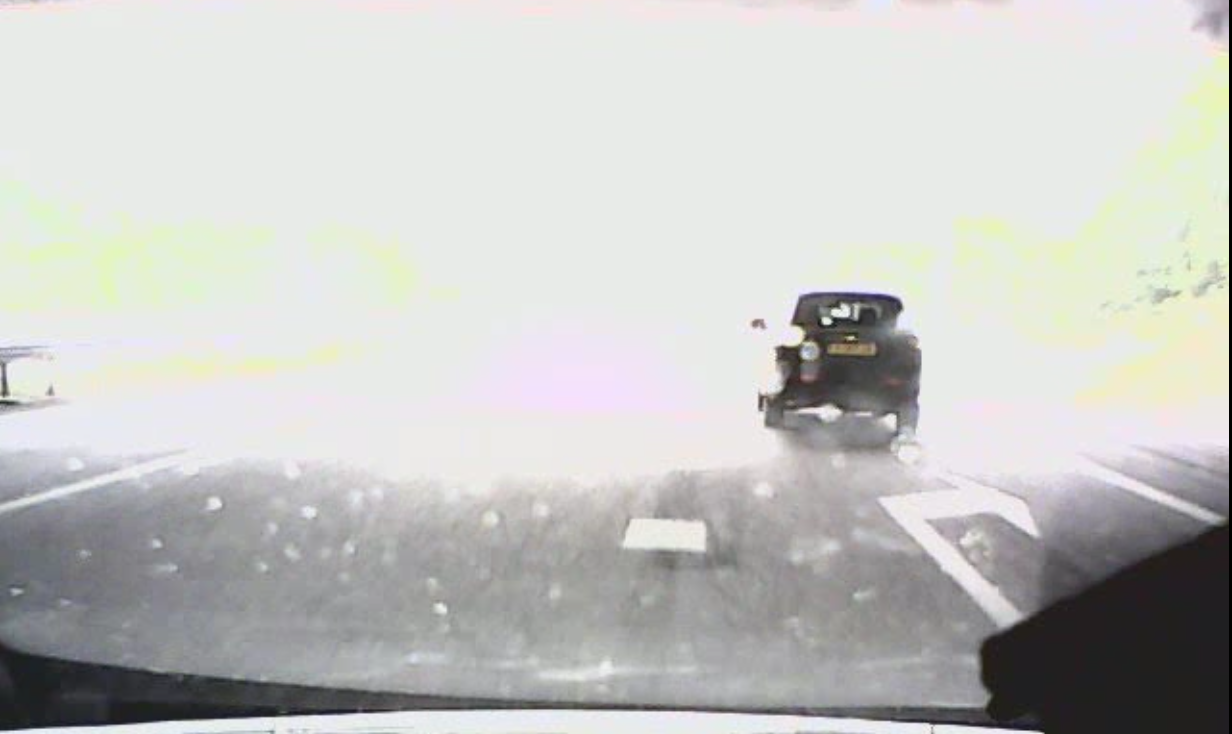
\includegraphics[width=\linewidth]{figures/glare}
	\caption{\cstarta The ego vehicle passes a flyover during daytime while performing a lane change. This causes glare such that the distance to the lane lines are not available. 
	%By using the previous and next available measurements, our proposed method is still able to detect the lane change.
	\cenda}
	\label{fig:glare}
\end{figure}



\subsection{Longitudinal activity of other vehicle}
\label{sec:longitudinal other vehicles}

The longitudinal activities of other vehicles are estimated in a similar manner as for the ego vehicle. However, instead of the speed of the ego vehicle, $\speed{\sample}$, the speed of the other vehicles is used. The ego vehicle measures the relative speed of other vehicles. Let $\speedtargetirel{\sample}{\indextarget}$ denote the relative speed of the $\indextarget$-th vehicles at sample $\sample$. The absolute speed of other vehicles is estimated by adding $v(k)$ to the estimated relative speed:
\begin{equation}
	\speedtargetiabs{\sample}{\indextarget} = \speedtargetirel{\sample}{\indextarget} + \speed{\sample}.
\end{equation}
To compute the longitudinal activities of the $\indextarget$-th vehicle, the approach outlined in \cref{sec:longitudinal ego} is used with $\speedtargetiabs{\sample}{\indextarget}$ substituted for $\speed{\sample}$. 

\begin{remark}
	\label{rem:no target}
	\cstarta Typically, $\speedtargetirel{\sample}{\indextarget}$ is obtained by fusing the outputs of several sensors \autocite{elfring2016effective}. 
	%How this is done is out of scope of this paper. 
	If $\speedtargetirel{\sample}{\indextarget}$ is not available, e.g., because the vehicle moved out of the view of the ego vehicle's sensors, there are no activities estimated for the $\indextarget$-th vehicle at sample step $\sample$. \cenda
	\cstartc Consequently, no tags are applied for the $\indextarget$-th vehicle at sample step $\sample$. This applies for all tags of the other vehicles that are mentioned in \cref{tab:tags}.\cendc
\end{remark}



\subsection{Lateral activity of other vehicle}
\label{sec:lateral other vehicles}

\cstartc
For the lane changes of other vehicles, only the lane changes to and from the ego vehicle's lane are considered.
To detect a lane change of the $\indextarget$-th vehicle, we use the distance of the $\indextarget$-th vehicle toward the ego vehicle's left and right lane lines, denoted by $\linelefttarget{\sample}{\indextarget}$ and $\linerighttarget{\sample}{\indextarget}$, respectively\cendc\cstartd\footnote{\cstartd $\linelefttarget{\sample}{\indextarget}$ and $\linerighttarget{\sample}{\indextarget}$ are determined by subtracting the estimated lane line positions from the estimated lateral position of the $\indextarget$-th vehicle. The lane line positions are based on the estimated shape of the lane lines. For more details, we refer the reader to \autocite{elfring2016effective}.\cendd}\cendd\cstartc.
We define $\linelefttargetinc{\sample}{\indextarget}$, $\linerighttargetinc{\sample}{\indextarget}$, $\linelefttargetdec{\sample}{\indextarget}$, and $\linerighttargetdec{\sample}{\indextarget}$ similar as $\lineleftinc{\sample}$ and $\lineleftdec{\sample}$ in \cref{eq:line left inc,eq:line left dec}.

A lane change is detected if the vehicle crosses either of the two lane lines.
There are four possible ways this can happen.
For now, we consider a right lane change toward the ego vehicle's lane.
A right lane change of the $\indextarget$-th vehicle toward the ego vehicle's lane is detected at sample step $\sample$ if the vehicle is not already changing lane and
\begin{equation}
	\label{eq:detect lane change target}
	\linelefttarget{\sample-1}{\indextarget} \leq 0 \land \linelefttarget{\sample}{\indextarget} > 0,
\end{equation}
where $\land$ indicates that both of the two conditions need to be satisfied.

To determine the start of the lane change, the lateral speed should be below the threshold $\lanechangespeed$ or --- in case the vehicle changes several lanes --- the lateral movement should be above a certain threshold (controlled by $\factorgoalmax$).
Because it might happen that the lateral speed is below the threshold during the whole lane change, a minimum lateral movement is considered as well (controlled by $\factorgoalmin$). 
As a result, the start of a right lane change toward the ego vehicle's lane is estimated to occur at sample step
\begin{multline}
	\label{eq:start lane change target}
	\arg \max_{\sampledummy < \sample} \left\{ \sampledummy: \linelefttarget{\sampledummy}{\indextarget} < -\factorgoalmax\widthlanetarget{\sample}{\indextarget} \lor \right. \\
	\left. \left( \linelefttargetinc{\sampledummy}{\indextarget} < \lanechangespeed\samplehorizon\sampletime \land \linelefttarget{\sampledummy}{\indextarget} < -\factorgoalmin\widthlanetarget{\sample}{\indextarget} \right) \right\}.
\end{multline}
Here, $\widthlanetarget{\sample}{\indextarget}=\linelefttarget{\sample}{\indextarget}-\linerighttarget{\sample}{\indextarget}$ is the estimated lane width. 
The end of the same lane change is estimated, in a similar way, to occur at sample step:
\begin{multline}
	\label{eq:end lane change target}
	\arg \max_{\sampledummy > \sample} \left\{ \sampledummy: \linelefttarget{\sampledummy}{\indextarget} > \factorgoalmax\widthlanetarget{\sample}{\indextarget} \lor \right. \\
	\left. \left(\linelefttargetinc{\sampledummy+\samplehorizon}{\indextarget} < \lanechangespeed\samplehorizon\sampletime \land \linelefttarget{\sampledummy}{\indextarget} > \factorgoalmin\widthlanetarget{\sample}{\indextarget}\right) \right\}.
\end{multline}

For a right lane change from the ego vehicle's lane, $\linerighttarget{\cdot}{\indextarget}$ and $\linerighttargetinc{\cdot}{\indextarget}$ are substituted for $\linelefttarget{\cdot}{\indextarget}$ and $\linelefttargetinc{\cdot}{\indextarget}$, respectively, in \cref{eq:detect lane change target,eq:start lane change target,eq:end lane change target}. 
Similarly, for a left lane change to the ego vehicle's lane, $-\linerighttarget{\cdot}{\indextarget}$ and $-\linerighttargetdec{\cdot}{\indextarget}$ are substituted for $\linelefttarget{\cdot}{\indextarget}$ and $\linelefttargetinc{\cdot}{\indextarget}$ in \cref{eq:detect lane change target,eq:start lane change target,eq:end lane change target}.
Finally, for a left lane change from the ego vehicle's lane, $-\linelefttarget{\cdot}{\indextarget}$ and $-\linelefttargetdec{\cdot}{\indextarget}$ are substituted for $\linelefttarget{\cdot}{\indextarget}$ and $\linelefttargetinc{\cdot}{\indextarget}$ in \cref{eq:detect lane change target,eq:start lane change target,eq:end lane change target}.
\cendc



\cstartc
\subsection{Longitudinal state of other vehicle}
\label{sec:longitudinal state other vehicle}

For the longitudinal state of any other vehicle, two possibilities are considered: in front of the ego vehicle or behind the ego vehicle. 
Let the longitudinal position at sample step $\sample$ of the $\indextarget$-th vehicle relative to the ego vehicle be denoted by $\lontarget{\sample}{\indextarget}$. 
The tag ``in front of ego'' applies when $\lontarget{\sample}{\indextarget}> 0$ and the tag ``behind ego'' applies when $\lontarget{\sample}{\indextarget}\leq 0$. 



\subsection{Lateral state of other vehicle}
\label{sec:lateral state other vehicle}

Four different possibilities are considered for the lateral state of any other vehicle. 
The lateral state is based on the estimated distance of the other vehicle toward the ego vehicle's lane lines, see \cref{tab:lateral state other vehicle}. 
The situation of $\linelefttarget{\sample}{\indextarget} < 0$ and $\linerighttarget{\sample}{\indextarget} \geq 0$ would mean that the other vehicle is left of the left lane line and right of the right lane line, so it is unclear in which lane the vehicle is.
%This generally only happens when there is a large error in either $\linelefttarget{\sample}{\indextarget}$ or $\linerighttarget{\sample}{\indextarget}$ because, e.g., the other vehicle is far away from the ego vehicle.

\begin{table}
	\centering
	\caption{\cstartc Lateral state based on $\linelefttarget{\sample}{\indextarget}$ and $\linerighttarget{\sample}{\indextarget}$.\cendc}
	\label{tab:lateral state other vehicle}
	\cstartc
	\begin{tabular}{lcc}
		\toprule
		& $\linelefttarget{\sample}{\indextarget} < 0$ & $\linelefttarget{\sample}{\indextarget} \geq 0$ \\ \otoprule		$\linerighttarget{\sample}{\indextarget} < 0$ & Left of ego & Same lane as ego \\
		$\linerighttarget{\sample}{\indextarget} \geq 0$ & Unclear & Right of ego \\
		\bottomrule
	\end{tabular}
	\cendc
\end{table}



\subsection{Lead vehicle}
\label{sec:lead vehicle}

Two possibilities are considered: a vehicle is a lead vehicle (the tag ``leader'' applies) or not (the tag ``no leader'' applies). A vehicle $\indextarget$ is considered as a lead vehicle at sample step $\sample$ if all of the following conditions are satisfied:
\begin{itemize}
	\item The vehicle is in front of the ego vehicle, i.e., $\lontarget{\sample}{\indextarget}>0$.
	\item The vehicle drives in the same lane as the ego vehicle, i.e., $\linelefttarget{\sample}{\indextarget} \geq 0$ and $\linerighttarget{\sample}{\indextarget} < 0$.
	\item The time headway of the ego vehicle toward the other vehicle, i.e., $\lontarget{\sample}/\speed{\sample}$ is less than the parameter $\thw>0$.
	\item There is no other vehicle that is closer to the ego vehicle while satisfying the above conditions, i.e., $\lontarget{\sample}{\indextarget} < \lontarget{\sample}{\indextargetother}$ for all $\indextargetother$-th vehicles with $\indextargetother \ne \indextarget$ that satisfy the above conditions.
\end{itemize}
\cendc



\subsection{Static environment}
\label{sec:static environment}

\cstartc
The aspect of the static environment that is considered in this paper is whether the ego vehicle drives on the highway or not. The location of the ego vehicle, based on GPS measurements, is used to determine the road the ego vehicle is driving on based on OpenStreetMaps\footnote{\cstartc See \url{https://www.openstreetmap.org/}.\cendc}. If the road is classified as ``motorway'' (see \autocite{osm_highway} for all possibilities), the tag ``highway'' is applied. Otherwise, the tag ``no highway'' is used.
\cendc

\section{Mining scenarios using tags}
\label{sec:mining}

\cstartd
For the scenario mining, we formulate a scenario category using a combination of tags.
As an example, \cref{fig:cutin formulation tags} shows how the scenario category ``cut in'' can be formulated using tags.
To further structure the tags, we formulate a scenario category as a sequence of \emph{items} where each \emph{item} corresponds to a combination of tags for all relevant subjects.
The number of items may vary from scenario category to scenario category.
The scenario category ``cut in'' in \cref{fig:cutin formulation tags} contains two items and considers a vehicle other than the ego vehicle that changes lane (other vehicle, item 1 and 2) and becomes the lead vehicle (other vehicle, item 2).
In the meantime, the ego vehicle follows its lane (ego vehicle, items 1 and 2) and the scenario category only considers highway driving (static environment, items 1 and 2).
When describing the tags for each item, logical AND, OR, or NOT rules may be used. 
For example, for the other vehicle in \cref{fig:cutin formulation tags}, either the tag ``changing lane left'' \emph{or} the tag ``changing lane right'' needs to apply.
\cendd

\begin{figure}
	\centering
	\setlength{\itemwidth}{5.5em}
\begin{tikzpicture}
% Ego vehicle.
\node[block, text width=\subjectwidth-1em, minimum width=\subjectwidth, fill=egocolor] at (-\descriptionwidth, 0) {Ego vehicle};
\node[block, text width=\descriptionwidth-1em, minimum width=\descriptionwidth, fill=egocolor] at (0, 0) {Lateral activity};
\node[tagitemtwo, fill=egocolor] at (0, 0) {Following lane};

% Other vehicle, lateral activity.
\node[block, text width=\subjectwidth-1em, minimum width=\subjectwidth, fill=othervehicle, minimum height=2\tagheight] at (-\descriptionwidth, -\tagheight-\tagsep) {Other vehicle};
\node[block, text width=\descriptionwidth-1em, minimum width=\descriptionwidth, fill=othervehicle] at (0, -\tagheight-\tagsep) {Lateral activity};
\node[tagitemtwo, fill=othervehicle] at (0, -\tagheight-\tagsep) {Changing lane left OR Changing lane right};

% Other vehicle, lead vehicle.
\node[block, text width=\descriptionwidth-1em, minimum width=\descriptionwidth, fill=othervehicle] at (0, -2\tagheight-\tagsep) {Lead vehicle};
\node[tagitem, fill=othervehicle] at (0, -2\tagheight-\tagsep) {No leader};
\node[tagitem, fill=othervehicle] at (\itemwidth, -2\tagheight-\tagsep) {Leader};

% Static environment.
\node[block, text width=\subjectwidth-1em, minimum width=\subjectwidth, fill=staticenvironment] at (-\descriptionwidth, -3\tagheight-2\tagsep) {Static environment};
\node[block, text width=\descriptionwidth-1em, minimum width=\descriptionwidth, fill=staticenvironment] at (0, -3\tagheight-2\tagsep) {On highway};
\node[tagitemtwo, fill=staticenvironment] at (0, -3\tagheight-2\tagsep) {Highway};

% Items.
\foreach \i in {1, 2} {%
	\node[minimum width=\itemwidth, align=center, minimum height=\itempos, anchor=north east] at (\i\itemwidth, \itempos) {Item \i};
	\draw[showitem] (\i\itemwidth, 0) -- (\i\itemwidth, \itempos);
}
\draw[showitem] (0, 0) -- (0, \itempos);
\end{tikzpicture}
	\caption{\cstartd Formulation of the scenario category ``cut in'' using tags.\cendd}
	\label{fig:cutin formulation tags}
\end{figure}


\cstartb
% Introduce n-grams and quickly explain what an n-gram is.
%For the scenario mining, we will employ n-grams and n-gram models. An n-gram is a sequence of $\nofngram$ items. 
%For example, in the field of natural language processing --- where n-grams are a popular modeling technique \autocite{hull1982experiments, brown1992class} --- each item might correspond to a single word.
%In our case, an item corresponds to a combination of tags. 
%
%% Explain that we use multiple n-gram models.
%% What are the advantages of using multiple n-grams?
%Instead of constructing one n-gram model with all tags within one data set, we construct different n-gram models for the different subjects. A subject could be, e.g., a road user or a static part of the environment. In this paper, we consider the subjects ``ego vehicle'', ``other vehicle'', and ``static environment''.
%Constructing different n-gram models instead of one n-gram model brings several benefits:
%\begin{itemize}
%	\item The number of possible items is much lower when considering only one subject that describes everything, such that it is more likely that most of the items are seen multiple times. 
%	As a result, analysis to predict tags or correct for wrong tags is possible \autocite{lesher1998optimal}.
%	\item If different tags are needed for mining (other) scenarios, only the n-gram models of the corresponding subjects need to be updated.
%	\item Searching for n-grams within the n-gram models is much faster since the n-gram models itself are much smaller.
%\end{itemize}
%
%% Explain items
%As mentioned before, an item corresponds to a combination of tags. 
%To further explain this, consider the following example: The ego vehicle cruises while following its lane. 
%At some point, the ego vehicle starts to accelerate before changing lane to the left. 
%Next, the ego vehicle starts cruising before the lane change is finished. 
%The corresponding tags are shown in \cref{fig:ego tags}.
%This example contains five items and each item starts and ends with an event, i.e., the start or end of an activity.
%The first item contains the tags ``cruising'' and ``following lane'', the second item contains the tags ``accelerating'' and ``following lane'', etc.

% Show how a scenario category is represented through a "template".
%To mine scenarios of a specific scenario category, we write a scenario category using n-grams. 
%To do this, the following rules apply:
%\begin{itemize}
%	\item For each subject that is considered in the scenario category, an n-gram is defined.
%	\item Each n-gram uses the same number of items ($\nofngram$). However, $\nofngram$ may vary from scenario category to scenario category.
%	\item For each item, the tags that apply are described. Logical AND or OR rules may apply.
%\end{itemize}
%
%\begin{table}
%	\centering
%	\caption{\cstartb N-grams that describe the scenario category ``cut in''. Because $\nofngram=2$, these are also called bigrams.\cendb}
%	\label{tab:ngrams cutin}
%	\cstartb
%	\begin{tabularx}{\linewidth}{p{5.5em}XX}
%		\toprule
%		Subject & Item 1 & Item 2 \\ \otoprule
%		Ego vehicle & Lateral activity: \newline Following lane & Lateral activity: \newline Following lane \\
%		Other vehicle & Lateral activity: \newline \{Changing lane left OR \newline \phantom{\{}Changing lane right\}\newline AND Lead vehicle: No & Lateral activity: \newline \{Changing lane left OR \newline \phantom{\{}Changing lane right\}\newline AND Lead vehicle: Yes \\
%		Static environment & On highway: Yes & On highway: Yes \\
%		\bottomrule
%	\end{tabularx}
%	\cendb
%\end{table}
%
%In \cref{tab:ngrams cutin}, the n-grams are shown for the scenario category ``cut-in''. 
%This scenario category considers a vehicle other than the ego vehicle that changes lane (other vehicle, item 1) and becomes the lead vehicle (other vehicle, item 2). 
%In the meantime the ego vehicle follows its lane (ego vehicle, items 1 and 2) and the scenario category only considers highway driving (static environment, items 1 and 2).

% How scenarios are mined using the template.
The scenarios are mined by searching for matches of the defined items within the tags of the data set. 
This searching is subject to two rules:
\begin{enumerate}
	\item For each item, there needs to be a match for all relevant subjects \emph{at the same sample time}.
	\item The different items need to occur \emph{right after each other}. 
\end{enumerate}\cendb
\cstartd To continue the example of the scenario category ``cut in'', \cref{fig:tags cut in} shows a part of labeled data in which a cut-in scenario is found. \cendd
\cstartb The two vertical dashed lines indicate the start and the end of the cut in that is defined in \cref{fig:cutin formulation tags}.
\cendb

\begin{figure*}
	\centering
	\setlength{\tagtotalwidth}{24em}
\setlength{\egovehiclefollowing}{15.5em}
\begin{tikzpicture}
% Ego vehicle.
\node[block, text width=\subjectwidth-1em, minimum width=\subjectwidth, fill=egocolor] at (-\descriptionwidth, 0) {Ego vehicle};
\node[block, text width=\descriptionwidth-1em, minimum width=\descriptionwidth, fill=egocolor] at (0, 0) {Lateral activity};
\node[tag, minimum width=\egovehiclefollowing, fill=egocolor] at (0, 0) {Following lane};
\node[tag, minimum width=\tagtotalwidth-\egovehiclefollowing, text width=\tagtotalwidth-\egovehiclefollowing-1em, fill=egocolor] at (\egovehiclefollowing, 0) {Changing lane left};

% Other vehicle, lateral activity.
\node[block, text width=\subjectwidth-1em, minimum width=\subjectwidth, fill=othervehicle, minimum height=2\tagheight] at (-\descriptionwidth, -\tagheight-\tagsep) {Other vehicle};
\node[block, text width=\descriptionwidth-1em, minimum width=\descriptionwidth, fill=othervehicle] at (0, -\tagheight-\tagsep) {Lateral activity};
\node[tag, text width=\otherfollowing-1em, minimum width=\otherfollowing, fill=othervehicle] at (0, -\tagheight-\tagsep) {Following lane};
\node[tag, text width=\otherchanging-1em, minimum width=\otherchanging, fill=othervehicle] at (\otherfollowing, -\tagheight-\tagsep) {Changing lane right};
\node[tag, text width=\tagtotalwidth-\otherfollowing-\otherchanging-1em, minimum width=\tagtotalwidth-\otherfollowing-\otherchanging, fill=othervehicle] at (\otherfollowing+\otherchanging, -\tagheight-\tagsep) {Following lane};

% Other vehicle, lead vehicle.
\node[block, text width=\descriptionwidth-1em, minimum width=\descriptionwidth, fill=othervehicle] at (0, -2\tagheight-\tagsep) {Lead vehicle};
\node[tag, minimum width=\othernolead, fill=othervehicle] at (0, -2\tagheight-\tagsep) {No leader};
\node[tag, minimum width=\tagtotalwidth-\othernolead, fill=othervehicle] at (\othernolead, -2\tagheight-\tagsep) {Leader};

% Static environment.
\node[block, text width=\subjectwidth-1em, minimum width=\subjectwidth, fill=staticenvironment] at (-\descriptionwidth, -3\tagheight-2\tagsep) {Static environment};
\node[block, text width=\descriptionwidth-1em, minimum width=\descriptionwidth, fill=staticenvironment] at (0, -3\tagheight-2\tagsep) {On highway};
\node[tag, minimum width=\tagtotalwidth, fill=staticenvironment] at (0, -3\tagheight-2\tagsep) {Highway};

% Show where the cut in is.
\draw[cutinline, dashed] (\otherfollowing, \cutinheight) -- (\otherfollowing, -4\tagheight-2\tagsep);
\draw[cutinline, dashed] (\egovehiclefollowing, \cutinheight) -- (\egovehiclefollowing, -4\tagheight-2\tagsep);
\draw[cutinline, <->] (\otherfollowing, \arrowheight) -- (\egovehiclefollowing, \arrowheight);
\node[anchor=north west, text width=\egovehiclefollowing-\otherfollowing-1em, minimum width=\egovehiclefollowing-\otherfollowing, minimum height=\cutinheight-\arrowheight, align=center] at (\otherfollowing, \cutinheight) {Cut in};

% Timeline.
\draw[timeline, ->] (0, -4\tagheight-2\tagsep-\timepos) -> (\tagtotalwidth, -4\tagheight-2\tagsep-\timepos);
\node[minimum width=\tagtotalwidth, align=center, anchor=north west, minimum height=\timepos] at (0, -4\tagheight-2\tagsep) {Time};
\end{tikzpicture}
%}

	\caption{\cstartc Example of tags describing a cut in. Note that only the tags that are relevant for the cut in, as defined in \cref{fig:cutin formulation tags}, are shown. \cendc\cstartf Furthermore, whereas there are multiple other vehicles around the ego vehicle, only the other vehicle that performs the cut in is shown.\cendf}
	\label{fig:tags cut in}
\end{figure*}




\section{Case study}
\label{sec:case study}

Here we illustrate the method by applying the method to the dataset described in \autocite{paardekooper2019dataset6000km}.

\begin{table}
	\centering
	\caption{\cstartc Values of parameters used in the case study. \cendc}
	\label{tab:parameters}
	\cstartc
	\begin{tabularx}{\linewidth}{lXl}
		\toprule
		Parameter & Description & Value \\ \otoprule
		$\sampletime$ & Sample time & \SI{0.01}{\second} \\
		$\samplehorizon$ & Sample window & 100 \\
		$\accelerationstart$ & Threshold determining the start of an acceleration or deceleration activity & \SI{0.1}{\meter\per\second\squared} \\
		$\accelerationcruise$ & Threshold determining the end of an acceleration or deceleration activity & \SI{0.1}{\meter\per\second\squared} \\
		$\speeddiff$ & Minimum speed increase/decrease for an acceleration/deceleration activity & \SI{1}{\meter\per\second} \\
		$\samplescruising$ & Minimum number of samples for cruising activity & 400 \\
		$\lanechangethreshold$ & A lane change is detected when the difference between consecutive lane line distances is larger than this threshold & \SI{1}{\meter} \\
		$\lanechangespeed$ & Threshold determining the start and end of a lane change & \SI{0.25}{\meter\per\second} \\
		$\factorgoalmax$ & Maximum factor of the lane width for a lane change of any other vehicle & 0.5 \\
		$\factorgoalmin$ & Minimum factor of the lane width for a lane change of any other vehicle & 0.1 \\
		\bottomrule
	\end{tabularx}
	\cendc
\end{table}

\begin{table*}
	\centering
	\caption{\cstartc N-grams that describe the scenario category ``overtaking before lane change''.\cendc}
	\label{tab:overtaking lane change}
	\cstartc
	\begin{tabularx}{\linewidth}{lXXX}
		\toprule
		Subject & Item 1 & Item 2 & Item 3 \\ \otoprule
		Ego vehicle & Lateral activity: Following lane & Lateral activity: Following lane & Lateral activity: Changing lane left \\
		Other vehicle & Lateral state: Left AND \newline Longitudinal state: Rear & Lateral state: Left AND \newline Longitudinal state: Front & Lateral state: Left AND \newline  Longitudinal state: Front \\
		Static environment & On highway: Yes & On highway: Yes & On highway: Yes \\
		\bottomrule
	\end{tabularx}
	\cendc
\end{table*}

\begin{table}
	\centering
	\caption{\cstartc N-grams that describe the scenario category ``lead vehicle braking''. The ego vehicle is not included in this table because there are no activities defined for the ego vehicle for this scenario category. \cendc}
	\label{tab:lead vehicle braking}
	\cstartc
	\begin{tabularx}{\linewidth}{lX}
		\toprule
		Subject & Item 1 \\ \otoprule
		Other vehicle & Longitudinal activity: Braking AND \newline Lead vehicle: Yes \\
		Static environment & On highway: Yes \\
		\bottomrule
	\end{tabularx}
	\cendc
\end{table}

\todo{Write case study setup. I will consider three different scenarios: Cut-in (as shown in \cref{tab:ngrams cutin}), overtaking before lane change (as shown in \cref{tab:overtaking lane change}), and lead vehicle braking (as shown in \cref{tab:lead vehicle braking}).}

\todo{I will consider changing the tables (\cref{tab:ngrams cutin,tab:overtaking lane change,tab:lead vehicle braking}) to figures that look more like \cref{fig:tags cut in}. It will be visually more attractive but it will also consume more space.}

\todo{Obtain results (this will require quite some time!)}

\todo{Write about the results.}

\section{Conclusions}
\label{sec:conclusions}

\todo{Write the conclusions. Perhaps also a short discussion?}



%\addtolength{\textheight}{-12cm}  % This command serves to balance the column lengths
                                  % on the last page of the document manually. It shortens
                                  % the textheight of the last page by a suitable amount.
                                  % This command does not take effect until the next page
                                  % so it should come on the page before the last. Make
                                  % sure that you do not shorten the textheight too much.

%\bibliographystyle{ieeetran}
%\bibliography{../bib}
\printbibliography



\end{document}
